% Options for packages loaded elsewhere
\PassOptionsToPackage{unicode}{hyperref}
\PassOptionsToPackage{hyphens}{url}
\PassOptionsToPackage{dvipsnames,svgnames,x11names}{xcolor}
%
\documentclass[
  letterpaper,
  DIV=11,
  numbers=noendperiod]{scrreprt}

\usepackage{amsmath,amssymb}
\usepackage{iftex}
\ifPDFTeX
  \usepackage[T1]{fontenc}
  \usepackage[utf8]{inputenc}
  \usepackage{textcomp} % provide euro and other symbols
\else % if luatex or xetex
  \usepackage{unicode-math}
  \defaultfontfeatures{Scale=MatchLowercase}
  \defaultfontfeatures[\rmfamily]{Ligatures=TeX,Scale=1}
\fi
\usepackage{lmodern}
\ifPDFTeX\else  
    % xetex/luatex font selection
\fi
% Use upquote if available, for straight quotes in verbatim environments
\IfFileExists{upquote.sty}{\usepackage{upquote}}{}
\IfFileExists{microtype.sty}{% use microtype if available
  \usepackage[]{microtype}
  \UseMicrotypeSet[protrusion]{basicmath} % disable protrusion for tt fonts
}{}
\makeatletter
\@ifundefined{KOMAClassName}{% if non-KOMA class
  \IfFileExists{parskip.sty}{%
    \usepackage{parskip}
  }{% else
    \setlength{\parindent}{0pt}
    \setlength{\parskip}{6pt plus 2pt minus 1pt}}
}{% if KOMA class
  \KOMAoptions{parskip=half}}
\makeatother
\usepackage{xcolor}
\setlength{\emergencystretch}{3em} % prevent overfull lines
\setcounter{secnumdepth}{5}
% Make \paragraph and \subparagraph free-standing
\makeatletter
\ifx\paragraph\undefined\else
  \let\oldparagraph\paragraph
  \renewcommand{\paragraph}{
    \@ifstar
      \xxxParagraphStar
      \xxxParagraphNoStar
  }
  \newcommand{\xxxParagraphStar}[1]{\oldparagraph*{#1}\mbox{}}
  \newcommand{\xxxParagraphNoStar}[1]{\oldparagraph{#1}\mbox{}}
\fi
\ifx\subparagraph\undefined\else
  \let\oldsubparagraph\subparagraph
  \renewcommand{\subparagraph}{
    \@ifstar
      \xxxSubParagraphStar
      \xxxSubParagraphNoStar
  }
  \newcommand{\xxxSubParagraphStar}[1]{\oldsubparagraph*{#1}\mbox{}}
  \newcommand{\xxxSubParagraphNoStar}[1]{\oldsubparagraph{#1}\mbox{}}
\fi
\makeatother


\providecommand{\tightlist}{%
  \setlength{\itemsep}{0pt}\setlength{\parskip}{0pt}}\usepackage{longtable,booktabs,array}
\usepackage{calc} % for calculating minipage widths
% Correct order of tables after \paragraph or \subparagraph
\usepackage{etoolbox}
\makeatletter
\patchcmd\longtable{\par}{\if@noskipsec\mbox{}\fi\par}{}{}
\makeatother
% Allow footnotes in longtable head/foot
\IfFileExists{footnotehyper.sty}{\usepackage{footnotehyper}}{\usepackage{footnote}}
\makesavenoteenv{longtable}
\usepackage{graphicx}
\makeatletter
\def\maxwidth{\ifdim\Gin@nat@width>\linewidth\linewidth\else\Gin@nat@width\fi}
\def\maxheight{\ifdim\Gin@nat@height>\textheight\textheight\else\Gin@nat@height\fi}
\makeatother
% Scale images if necessary, so that they will not overflow the page
% margins by default, and it is still possible to overwrite the defaults
% using explicit options in \includegraphics[width, height, ...]{}
\setkeys{Gin}{width=\maxwidth,height=\maxheight,keepaspectratio}
% Set default figure placement to htbp
\makeatletter
\def\fps@figure{htbp}
\makeatother

\usepackage{fontspec}
\usepackage{multirow}
\usepackage{multicol}
\usepackage{colortbl}
\usepackage{ulem}
\usepackage{hhline}
\newlength\Oldarrayrulewidth
\newlength\Oldtabcolsep
\usepackage{longtable}
\usepackage{array}
\usepackage{hyperref}
\usepackage{float}
\usepackage{wrapfig}
\KOMAoption{captions}{tableheading}
\makeatletter
\@ifpackageloaded{bookmark}{}{\usepackage{bookmark}}
\makeatother
\makeatletter
\@ifpackageloaded{caption}{}{\usepackage{caption}}
\AtBeginDocument{%
\ifdefined\contentsname
  \renewcommand*\contentsname{Table of contents}
\else
  \newcommand\contentsname{Table of contents}
\fi
\ifdefined\listfigurename
  \renewcommand*\listfigurename{List of Figures}
\else
  \newcommand\listfigurename{List of Figures}
\fi
\ifdefined\listtablename
  \renewcommand*\listtablename{List of Tables}
\else
  \newcommand\listtablename{List of Tables}
\fi
\ifdefined\figurename
  \renewcommand*\figurename{Figure}
\else
  \newcommand\figurename{Figure}
\fi
\ifdefined\tablename
  \renewcommand*\tablename{Table}
\else
  \newcommand\tablename{Table}
\fi
}
\@ifpackageloaded{float}{}{\usepackage{float}}
\floatstyle{ruled}
\@ifundefined{c@chapter}{\newfloat{codelisting}{h}{lop}}{\newfloat{codelisting}{h}{lop}[chapter]}
\floatname{codelisting}{Listing}
\newcommand*\listoflistings{\listof{codelisting}{List of Listings}}
\makeatother
\makeatletter
\makeatother
\makeatletter
\@ifpackageloaded{caption}{}{\usepackage{caption}}
\@ifpackageloaded{subcaption}{}{\usepackage{subcaption}}
\makeatother

\ifLuaTeX
  \usepackage{selnolig}  % disable illegal ligatures
\fi
\usepackage{bookmark}

\IfFileExists{xurl.sty}{\usepackage{xurl}}{} % add URL line breaks if available
\urlstyle{same} % disable monospaced font for URLs
\hypersetup{
  pdftitle={Morice River Watershed Connectivity Restoration Plan},
  pdfauthor={Canadian Wildlife Federation},
  colorlinks=true,
  linkcolor={blue},
  filecolor={Maroon},
  citecolor={Blue},
  urlcolor={Blue},
  pdfcreator={LaTeX via pandoc}}


\title{Morice River Watershed Connectivity Restoration Plan}
\author{Canadian Wildlife Federation}
\date{27-07-2026}

\begin{document}
\maketitle

\renewcommand*\contentsname{Table of contents}
{
\hypersetup{linkcolor=}
\setcounter{tocdepth}{1}
\tableofcontents
}

\bookmarksetup{startatroot}

\chapter*{Executive Summary}\label{executive-summary}
\addcontentsline{toc}{chapter}{Executive Summary}

\markboth{Executive Summary}{Executive Summary}

The purpose of the Morice River Watershed Connectivity Restoration Plan
(WCRP) is to improve understanding of habitat connectivity for Sockeye
Salmon (Onchorhynchus nerka), Chinook Salmon (O. tschawytscha), Coho
Salmon (O. kisutch) and steelhead (O. mykiss) (herein referred to as
`Pacific salmon and steelhead') in the Morice River and inform efforts
to close knowledge gaps and plan and prioritize restoration. Local data
and knowledge are combined with connectivity modelling to estimate
current connectivity status and identify structures that potentially
block the most habitat. This informs the prioritization of field
assessments to close the most significant knowledge gaps efficiently.
Information from field assessments of barrier status and habitat
condition are incorporated into the model, improving understanding of
which barriers block the most habitat, and informing restoration
prioritization. As knowledge gaps are closed and barriers are addressed,
this plan will be revised to summarize progress and provide updated
estimates of connectivity status and the status and relative importance
of remaining structures.

In the Morice River watershed, 878.78 km of Pacific salmon and steelhead
spawning habitat are currently connected to the ocean and 53.25 km are
disconnected from it. This means that 94.3\% of the 932.03 km of total
spawning habitat is connected. 1924.33 km of Pacific salmon and
steelhead rearing habitat are currently connected to the ocean and
167.07 km are disconnected from it. This means that 92.0\% of the 2091.4
km of total rearing habitat is connected.

In the Morice River watershed, 73 structures potentially disconnect
spawning habitat, and 139 structures potentially disconnect rearing
habitat for Pacific salmon and steelhead. Of these, 3 are identified as
barriers in need of rehabilitation (priority barriers), and 136 require
further field assessment.

\begin{figure}

\centering{

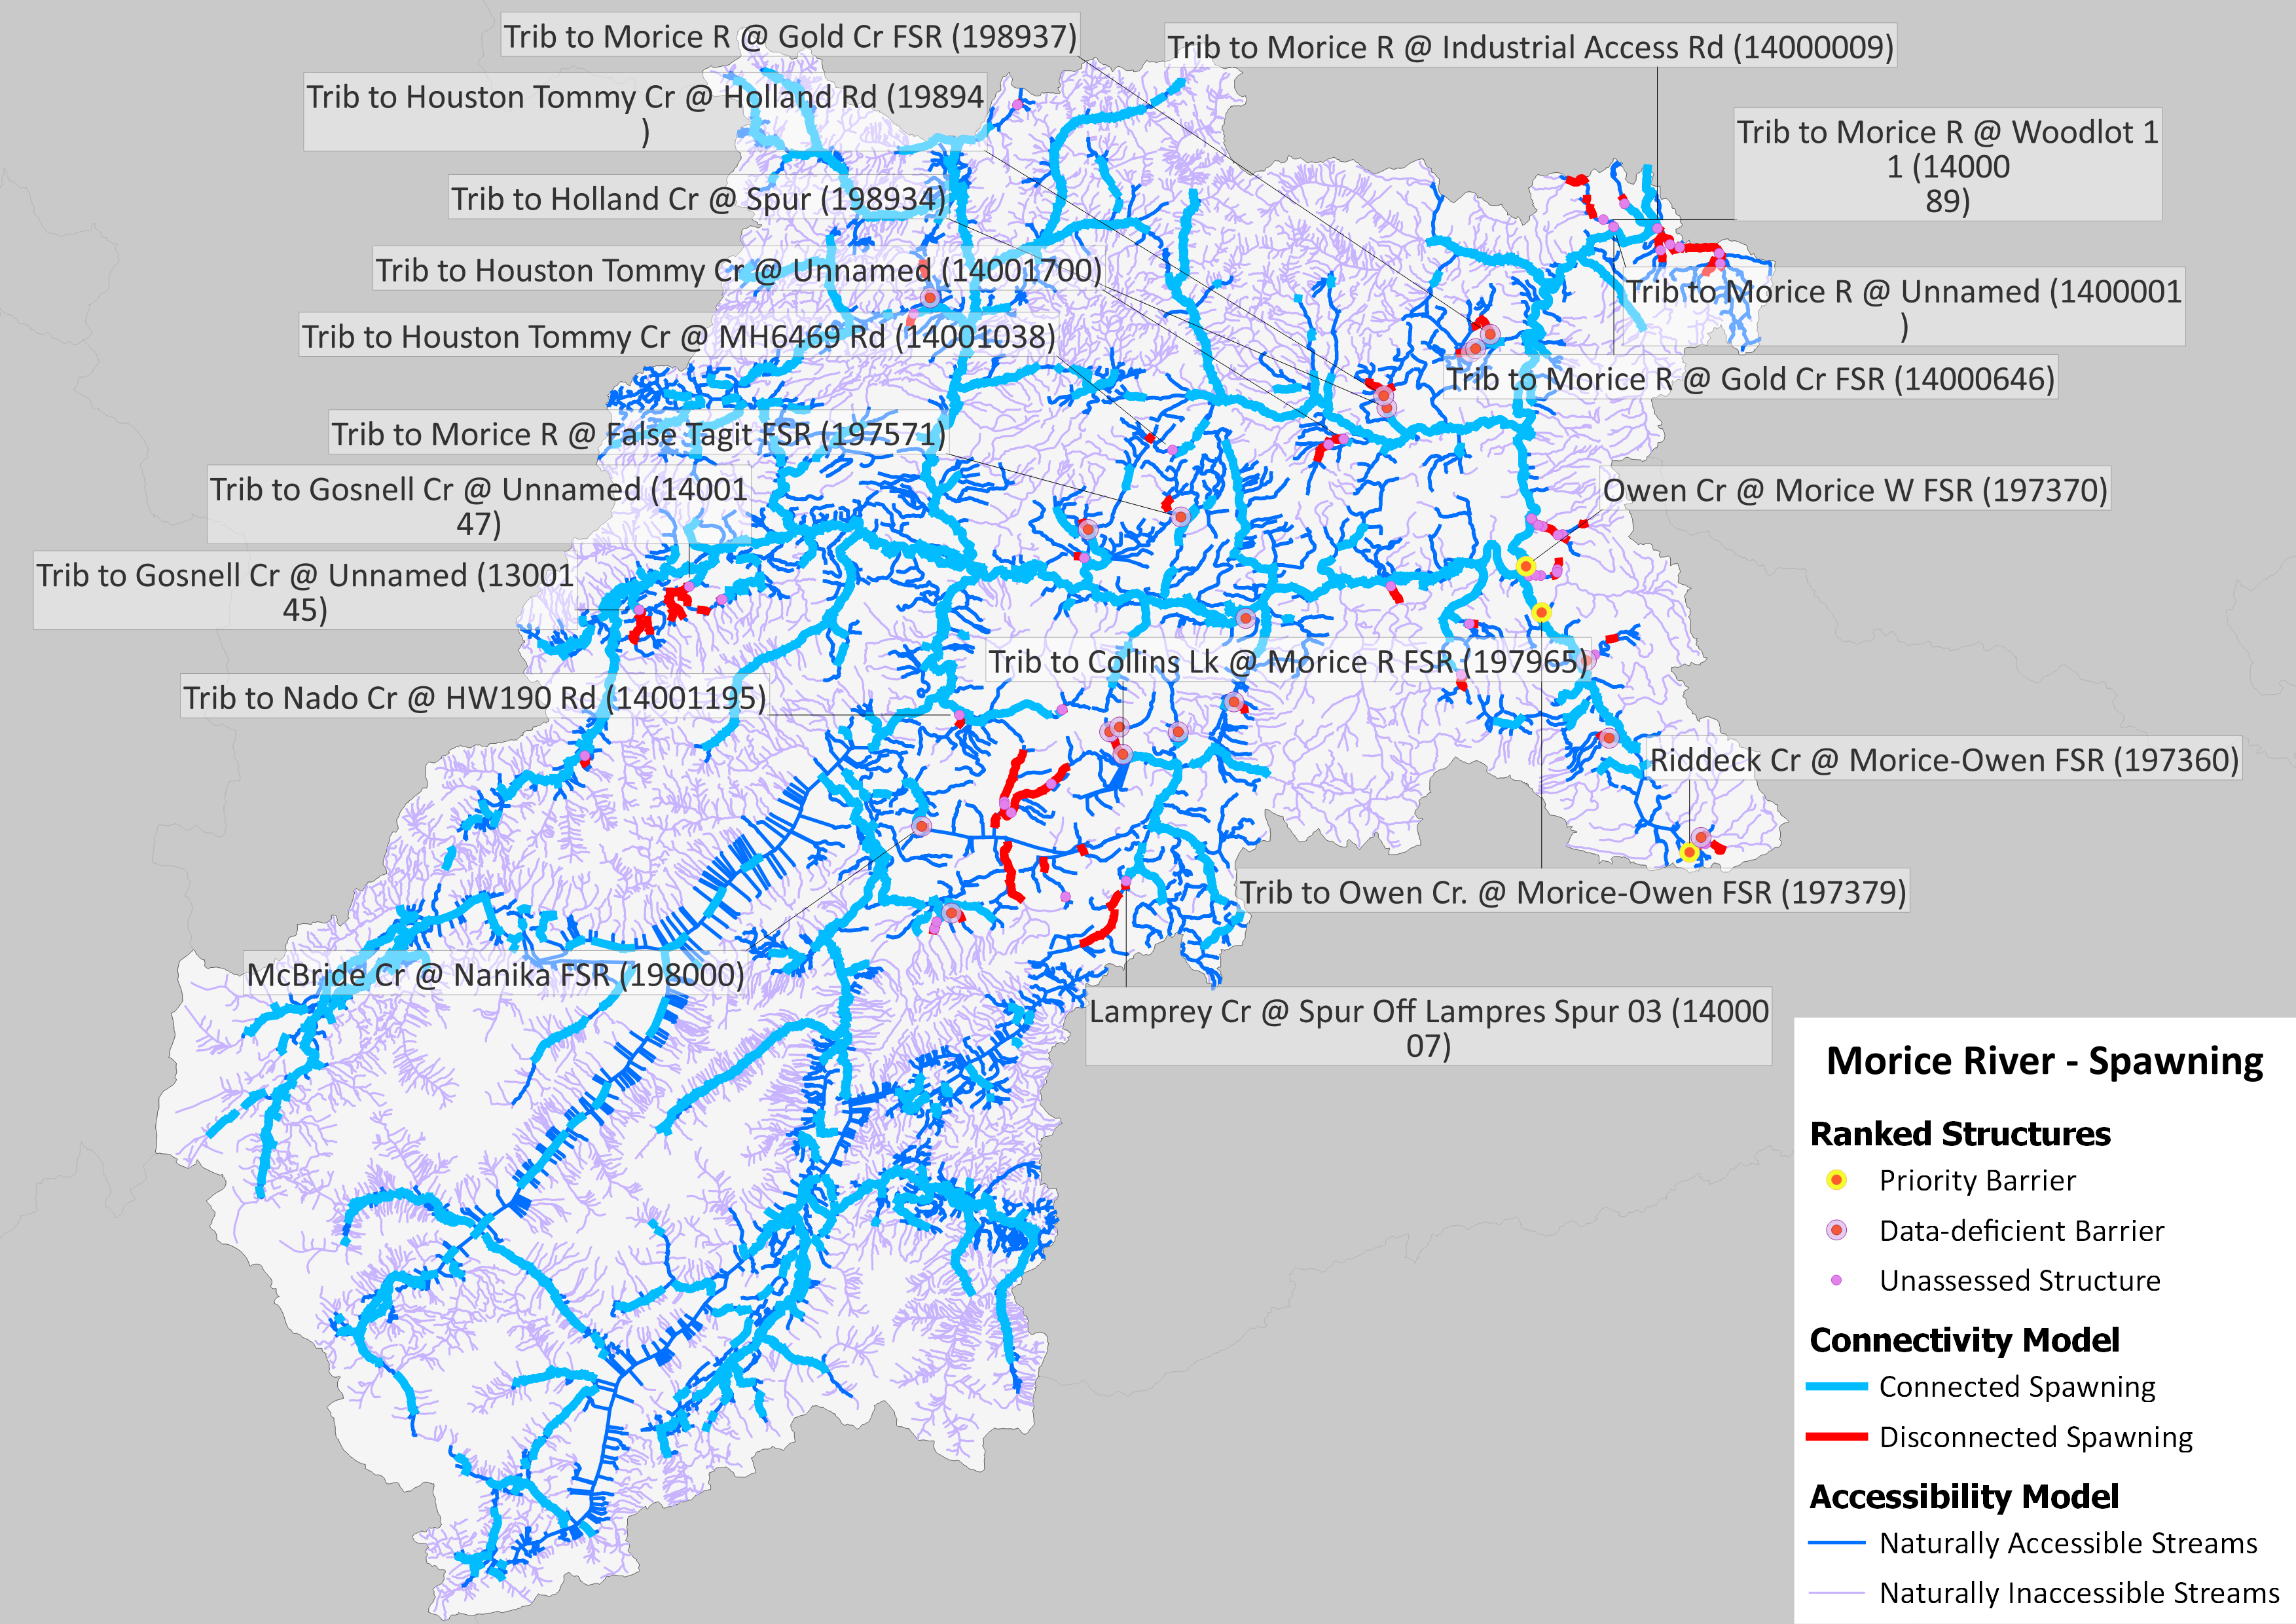
\includegraphics{content/images/Figure_1_Figure 5_spawning map.png}

}

\caption{\label{fig-map1}Map of Pacific salmon and steelhead spawning
habitat and structures that are confirmed or potential barriers to fish
passage in the Morice River watershed as of May 2026. Structure data
were obtained from BCFishPass and the Canadian Aquatic Barriers Database
(aquaticbarriers.ca). The accessibility model represents areas of the
watershed that one or more of Pacific salmon and steelhead could access
naturally in the absence of anthropogenic barriers. The habitat model
represents the subset of accessible waterbodies that may be used by one
or more Pacific salmon and steelhead for spawning. Available local
knowledge and data were incorporated and overruled habitat model
results. Thick red lines represent habitat considered to be fully
disconnected (upstream of barriers or unassessed structures).}

\end{figure}%

\begin{figure}

\centering{

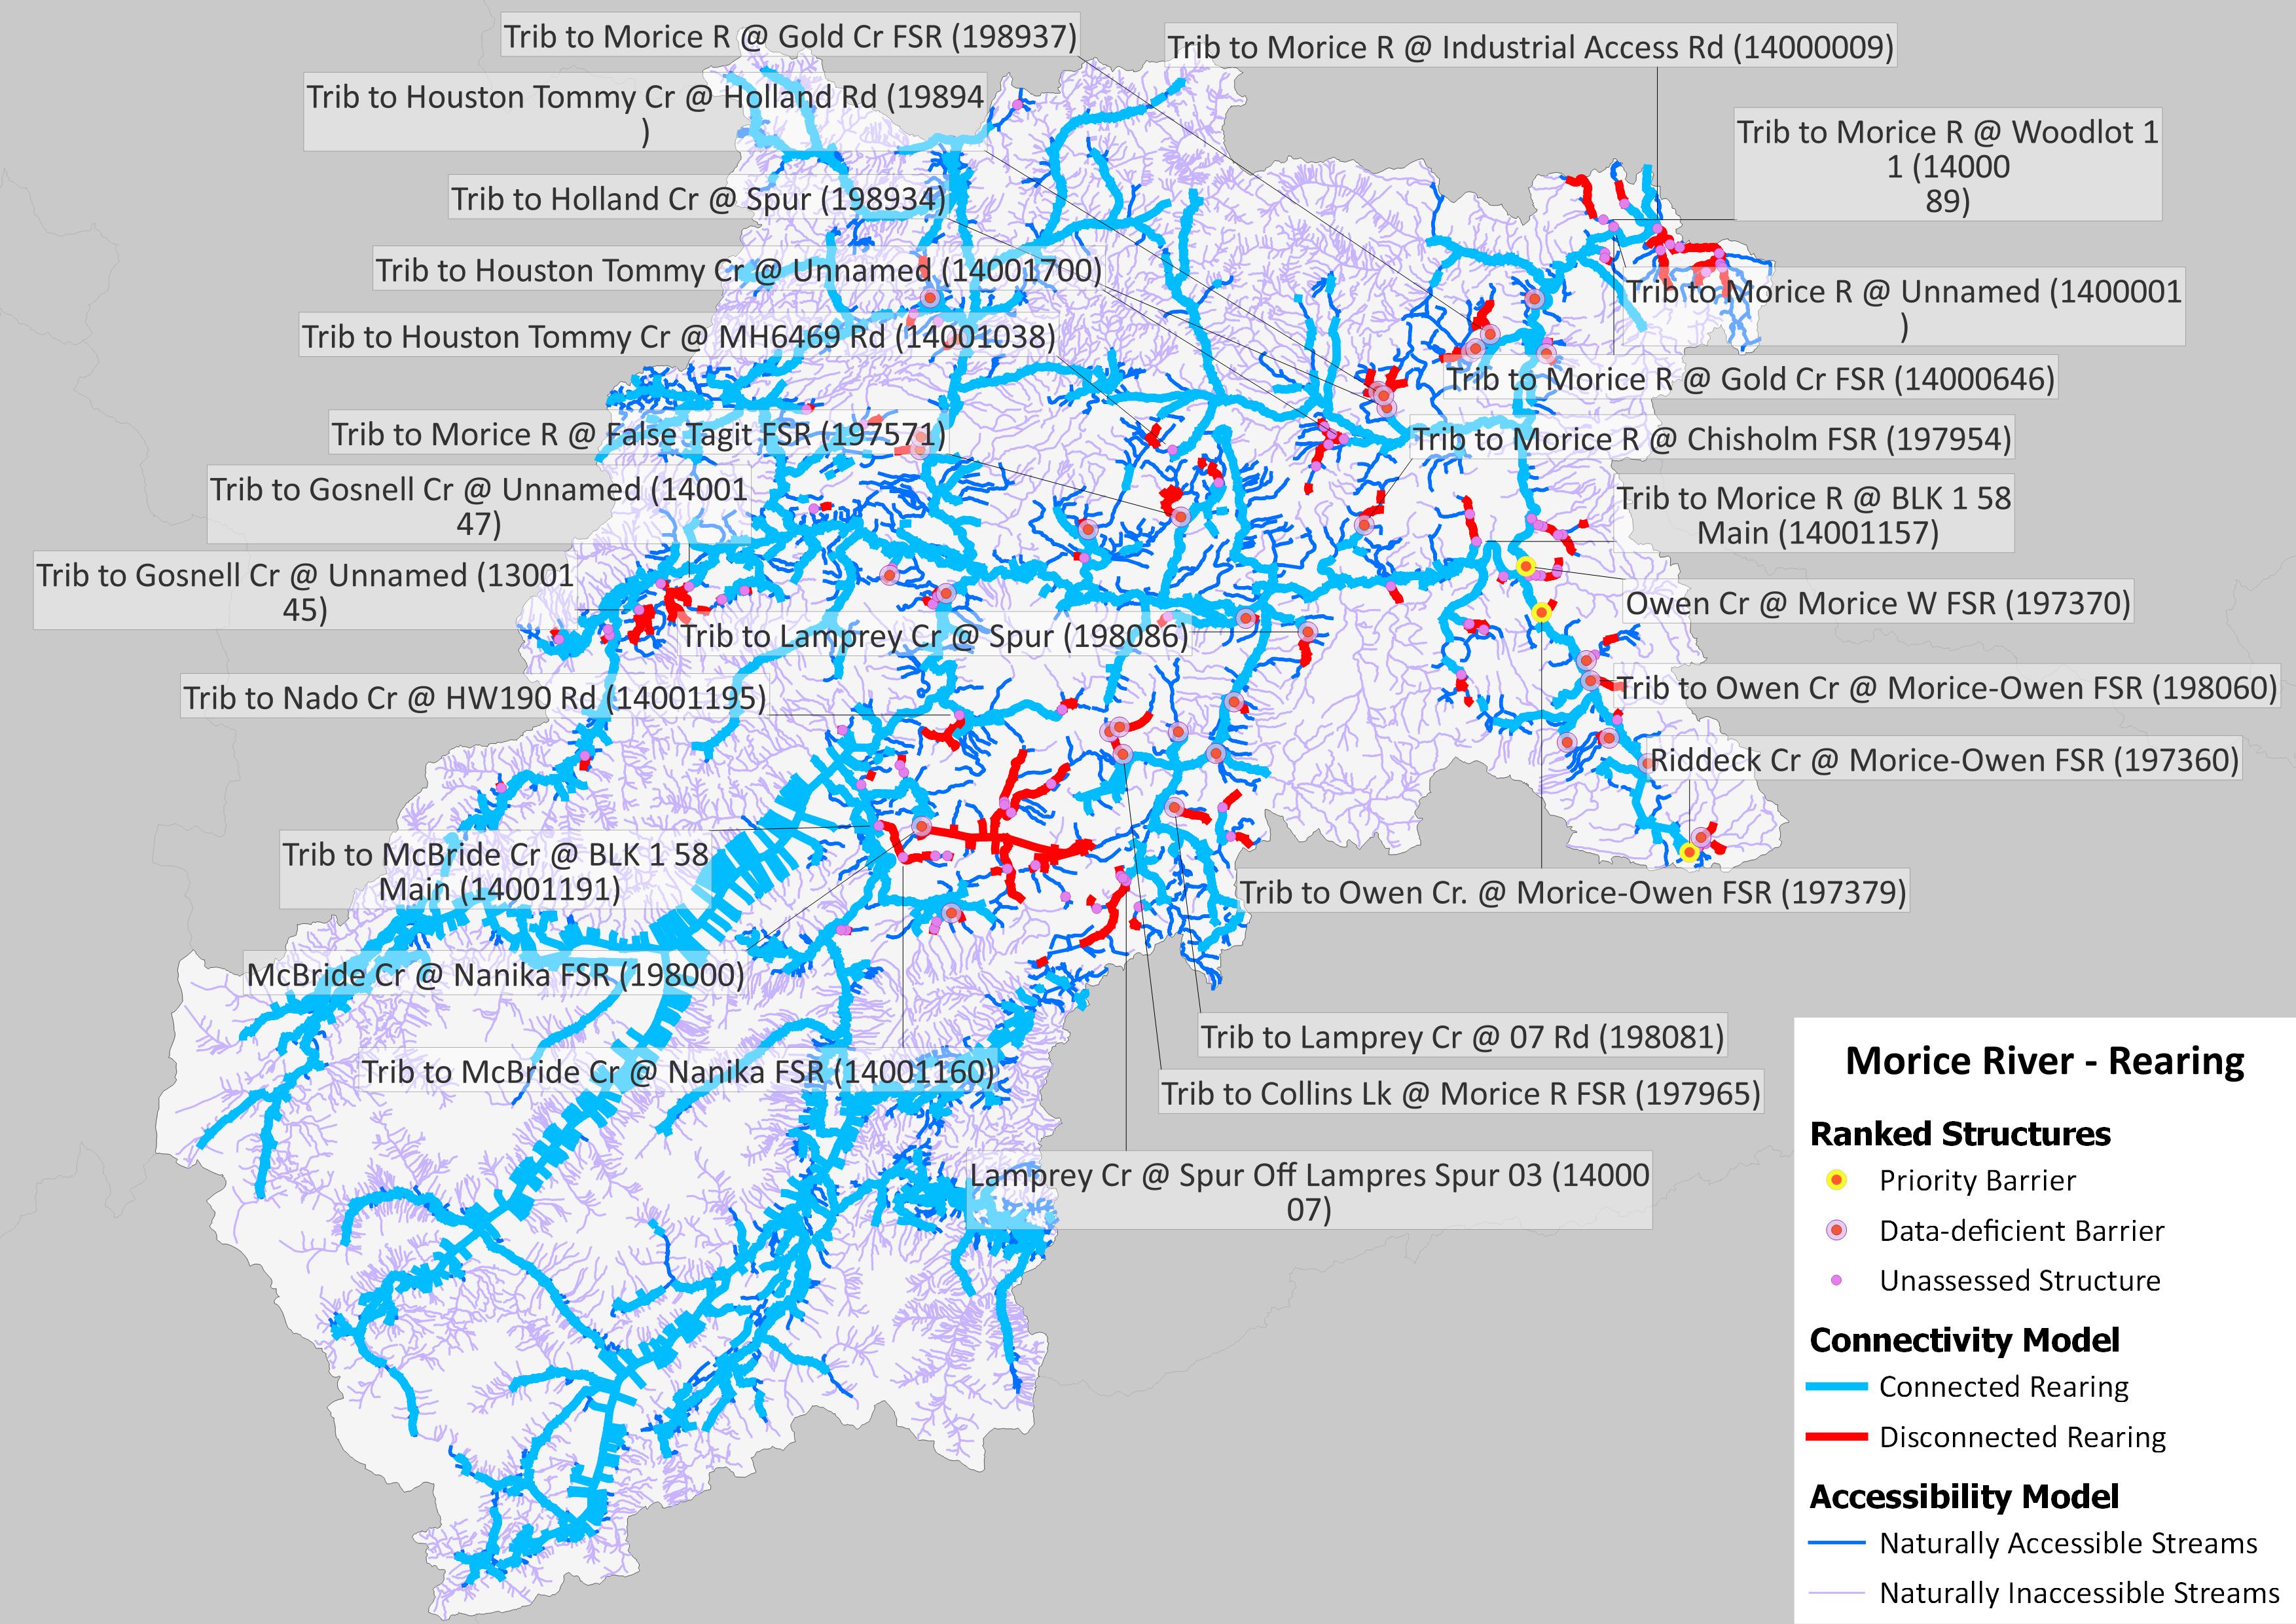
\includegraphics{content/images/Figure_2_Figure 6_rearing map.png}

}

\caption{\label{fig-map2}Map of Pacific salmon and steelhead rearing
habitat and structures that are confirmed or potential barriers to fish
passage in the Morice River watershed as of May 2026. Structure data
were obtained from BCFishPass and the Canadian Aquatic Barriers Database
(aquaticbarriers.ca). The accessibility model represents areas of the
watershed that one or more of Pacific salmon and steelhead could access
naturally in the absence of anthropogenic barriers. The habitat model
represents the subset of accessible waterbodies that may be used by one
or more Pacific salmon and steelhead for rearing. Available local
knowledge and data were incorporated and overruled habitat model
results. Thick red lines represent habitat considered to be fully
disconnected (upstream of barriers or unassessed structures).}

\end{figure}%

\begin{figure}

\centering{

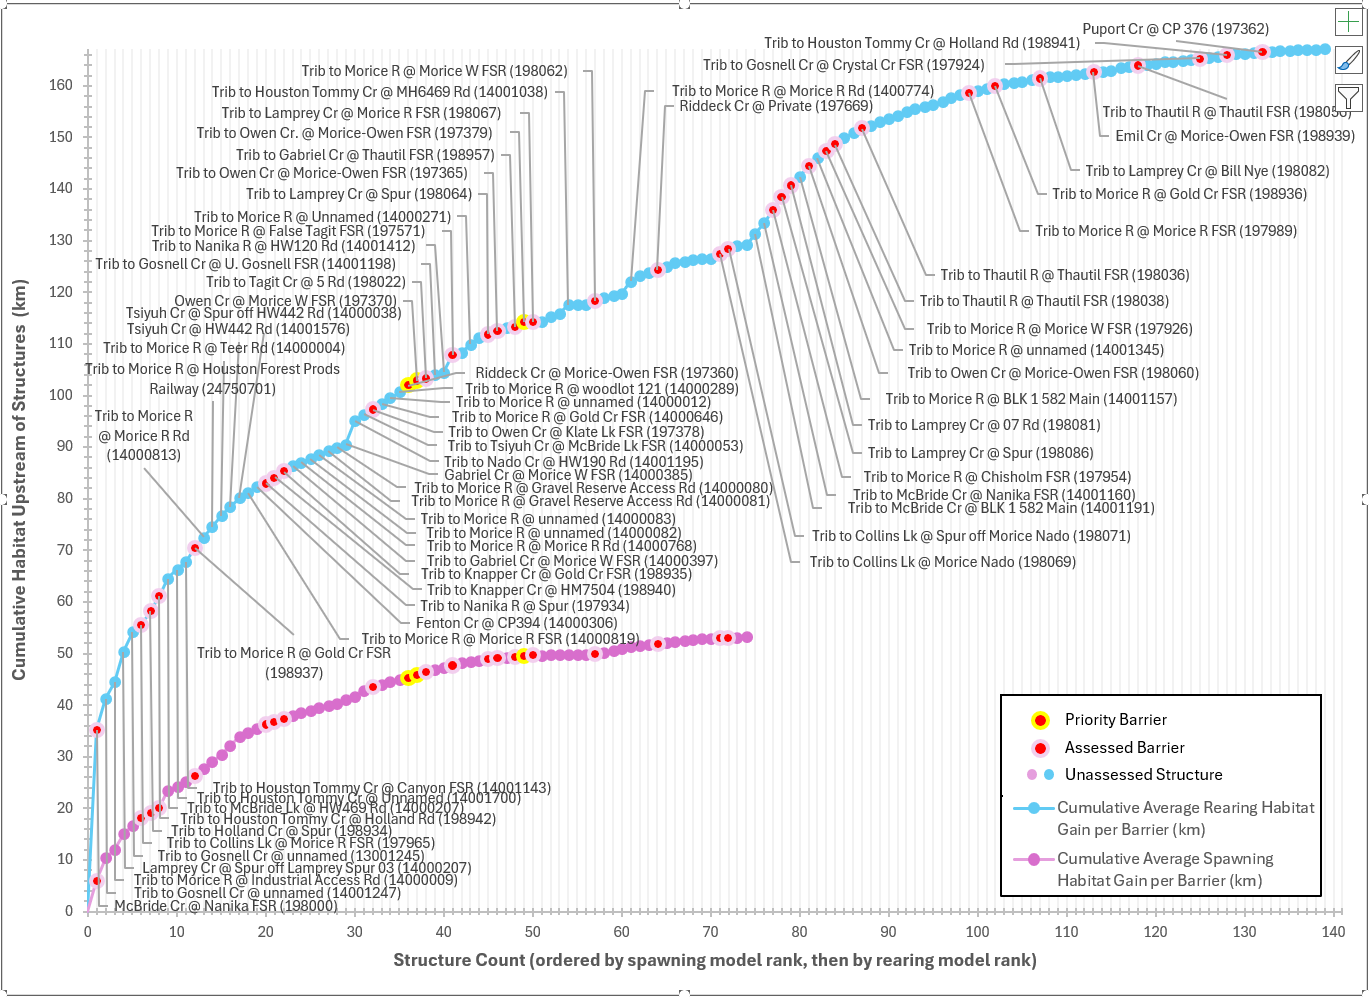
\includegraphics{content/images/Fig_3_Fig 7_MORR_HAC.png}

Habitat Accumulation Curve (HAC) showing structures in the Morice River
watershed as of May 2026. Structures are ranked based on how much (km)
spawning habitat for Pacific salmon and steelhead is upstream, then by
amount (km) of rearing habitat is upstream. Habitat upstream of
unassessed structures is considered disconnected until field assessments
are completed. Structures that were excluded as passable are not shown;
however, rehabilitated barriers are shown (where applicable) to
demonstrate the connectivity gains achieved through implementation of
this plan. :::

This WCRP was initiated in 2025, but concerted efforts towards
connectivity assessments and planning have been ongoing in the watershed
by key groups, including the Society for Ecological Restoration in
Northern BC, office of the Wet'suwet'en, BC Fish Passage Technical
Working Group, and Fisheries and Oceans Canada, among others, since
2020. Since then, the passability of X structures has been assessed, and
further habitat assessments were completed at X of these. Several
priority barriers have been identified through these processes, and
plans to begin restoring connectivity are underway, with a particular
focus on the Owen Creek (Bii Wenii Kwa) subwatershed.

\bookmarksetup{startatroot}

\chapter*{Introduction}\label{introduction}
\addcontentsline{toc}{chapter}{Introduction}

\markboth{Introduction}{Introduction}

\section*{Purpose}\label{purpose}
\addcontentsline{toc}{section}{Purpose}

\markright{Purpose}

This plan encompasses a portion of the traditional, unceded territories
of the Wet'suwet'en and Gitxsan peoples. \emph{Wedzin Kwah} means river
of clear, blue-green waters in Wet'suwet'en and refers to both the
Morice River and the lower Bulkley River and their tributaries, though
this plan covers only the Morice River portion of the \emph{Wedzin
Kwah}. The Bulkley River watershed is discussed in the
\href{https://bulkley-wcrp.netlify.app/}{Bulkley River WCRP}.

The purpose of the Morice River Watershed Connectivity Restoration Plan
(WCRP) is to improve understanding of habitat connectivity for Sockeye
Salmon (Onchorhynchus nerka), Chinook Salmon (O. tschawytscha), Coho
Salmon (O. kisutch) and steelhead (O. mykiss) (herein referred to as
`Pacific salmon and steelhead') in the Morice River watershed and inform
efforts to close knowledge gaps and plan and prioritize field
assessments and restoration.

Local data and knowledge are combined with connectivity modelling to
estimate current connectivity status and identify structures that
potentially block the most habitat. This informs the prioritization of
field assessments to close the most significant knowledge gaps
efficiently. Information from field assessments of barrier status and
habitat condition are incorporated into the model, improving
understanding of which barriers block the most habitat.

This information is also used to inform and plan restoration efforts.
Structure rankings inform restoration prioritization by summarizing what
is known about fragmentation and showing the relative amount of habitat
upstream of each barrier. Actual prioritization of restoration
activities is a social decision that requires additional information,
including the quality and condition of upstream habitat, the cultural
importance of different areas within the watershed, and the costs and
logistics of addressing each barrier relative to the ecological benefits
of doing so.

As knowledge gaps are closed and barriers are addressed, this plan is
revised to summarize progress and provide updated estimates of
connectivity status and the status and relative importance of remaining
structures.

\section*{Scope}\label{scope}
\addcontentsline{toc}{section}{Scope}

\markright{Scope}

This WCRP focuses on habitat connectivity for Pacific salmon and
steelhead in the Morice River watershed (Figure 4). Model outputs
include an estimate of the current connectivity status along with
structure ranks and counts, with Pacific salmon and steelhead
connectivity estimated for both spawning habitat and rearing habitat.

Connectivity models in this WCRP focus on longitudinal habitat
fragmentation by anthropogenic structures, including all types of dams
and stream crossings. Diffuse natural barriers that make entire areas
impassible are not included in the models but may be used to define the
scope of this WCRP. For example, a tributary that is inhospitable
because of increased water temperature may be excluded from the overall
spatial scope of the WCRP because restoration needs there are broader
than connectivity.

\begin{figure}
\centering
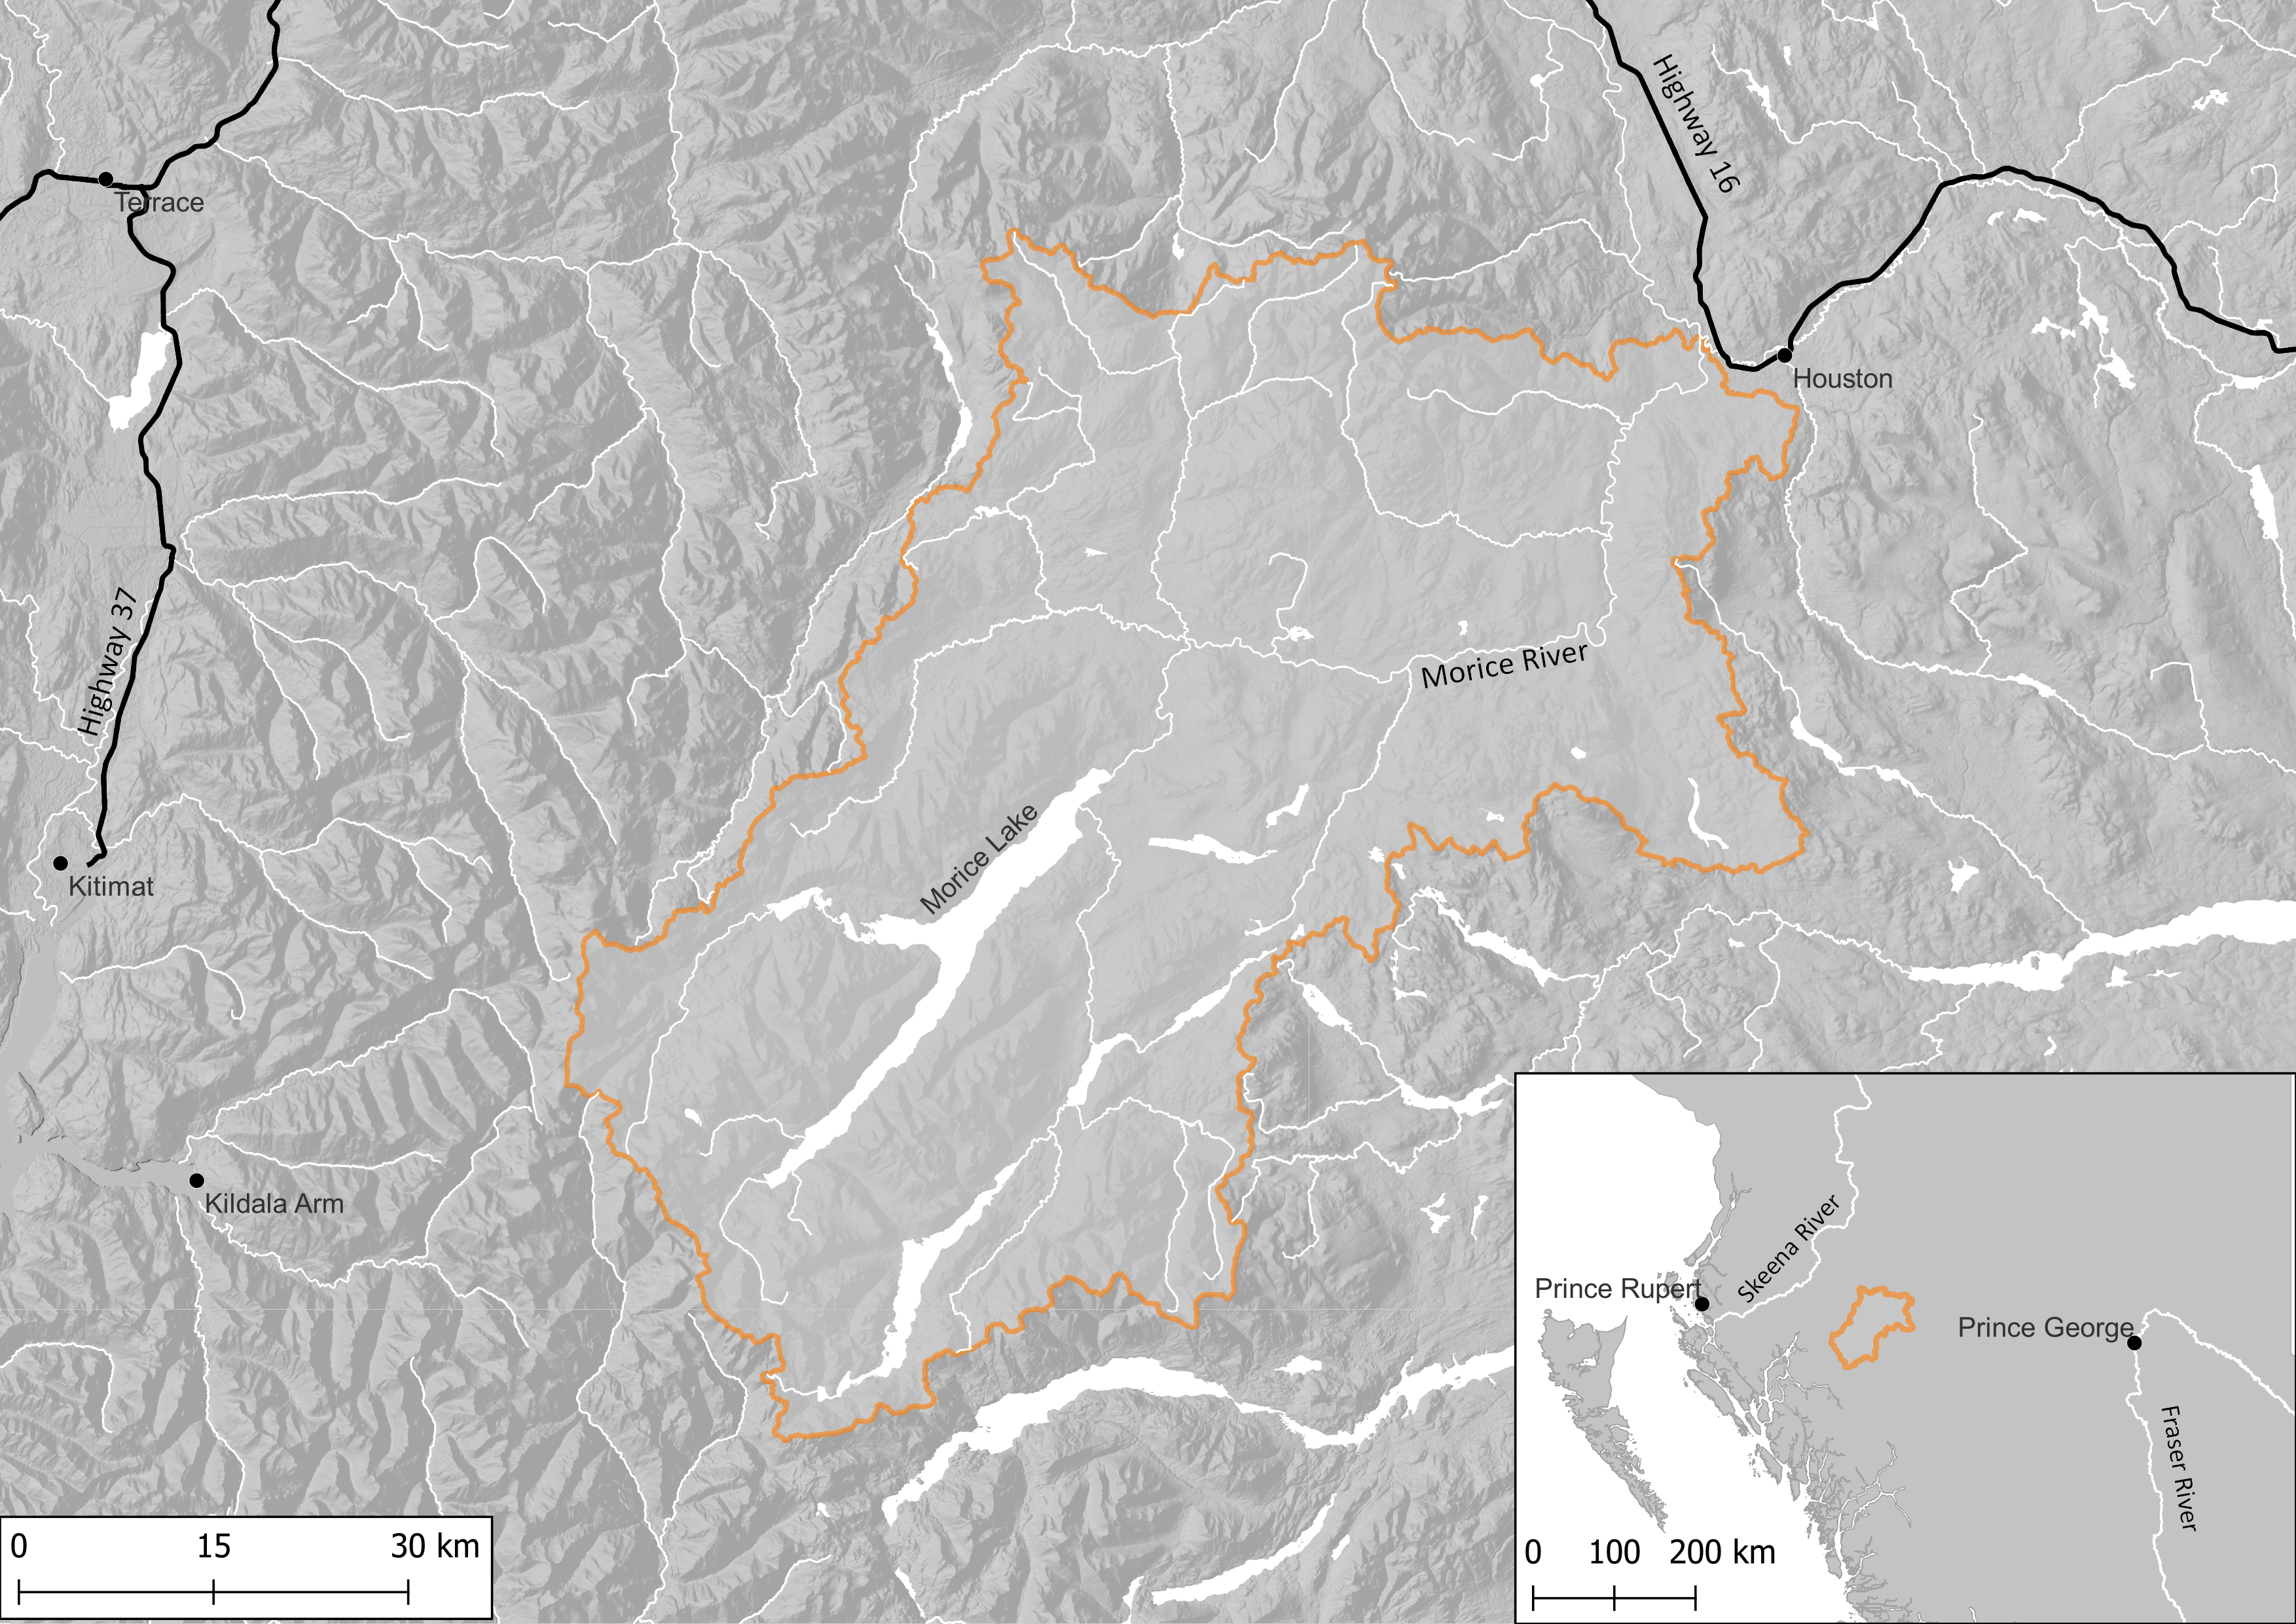
\includegraphics{content/images/Figure_4_morr_scope_map.png}
\caption{Figure 4: Map of the geographic scope of this connectivity
restoration plan for Pacific salmon and steelhead in the Morice River in
British Columbia.}
\end{figure}

\bookmarksetup{startatroot}

\chapter*{Glossary}\label{glossary}
\addcontentsline{toc}{chapter}{Glossary}

\markboth{Glossary}{Glossary}

\section*{General Terms}\label{general-terms}
\addcontentsline{toc}{section}{General Terms}

\markright{General Terms}

\subsection*{Freshwater connectivity}\label{freshwater-connectivity}
\addcontentsline{toc}{subsection}{Freshwater connectivity}

The degree to which aquatic species can move, disperse, or migrate
freely through freshwater systems.

\subsection*{Focal species or guilds}\label{focal-species-or-guilds}
\addcontentsline{toc}{subsection}{Focal species or guilds}

The ecologically and culturally important species (e.g., Westslope
Cutthroat Trout) or groups of species for which habitat connectivity is
being conserved or restored.

\subsection*{Structure}\label{structure}
\addcontentsline{toc}{subsection}{Structure}

A feature, either anthropogenic (e.g., culvert, dam) or a temporary
natural feature (e.g., barrier beach, debris jam) that may fragment
freshwater systems and limit the ability of species to disperse and/or
migrate freely within their naturally accessible habitat. Differentiated
from more permanent natural features, such as waterfalls, that delineate
naturally-accessible waterbodies.

\subsection*{Set of structures}\label{set-of-structures}
\addcontentsline{toc}{subsection}{Set of structures}

A set of two or more structures that must be addressed/considered
together to achieve a combined increase in habitat connectivity.

\subsection*{Current connectivity
status}\label{current-connectivity-status}
\addcontentsline{toc}{subsection}{Current connectivity status}

the measure (i.e., amount, proportion, or index) of habitat that is
currently connected for each focal species, assuming that all unassessed
structures are barriers.~

\subsection*{Rank}\label{rank}
\addcontentsline{toc}{subsection}{Rank}

The relative importance of a structure (individually and/or in sets)
based on the amount (km) of habitat blocked by it. For sets of
structures, the total amount of habitat blocked by the set is averaged
by the number of barriers in the set.

\subsection*{Habitat}\label{habitat}
\addcontentsline{toc}{subsection}{Habitat}

Key habitat that is likely to support important life stages for focal
species (i.e., spawning and rearing), rather than simply movement
corridors.

\section*{Structure Status Terms}\label{structure-status-terms}
\addcontentsline{toc}{section}{Structure Status Terms}

\markright{Structure Status Terms}

\subsection*{Unassessed structures}\label{unassessed-structures}
\addcontentsline{toc}{subsection}{Unassessed structures}

Mapped structures that have not been assessed in the field.

\subsection*{Excluded Structures}\label{excluded-structures}
\addcontentsline{toc}{subsection}{Excluded Structures}

Structures that were investigated and removed from consideration or the
model because they do not exist, are passable, or that no habitat was
found upstream.

\subsection*{Data-deficient barriers}\label{data-deficient-barriers}
\addcontentsline{toc}{subsection}{Data-deficient barriers}

Structures that have had some form of assessment but need further
investigation before a decision can be made as to whether they will be
listed as a priority.

\subsection*{Priority barrier}\label{priority-barrier}
\addcontentsline{toc}{subsection}{Priority barrier}

Structures that were assessed as barriers with habitat upstream, and for
which fish-passage rehabilitation is being pursued.

\subsection*{Non-actionable barriers}\label{non-actionable-barriers}
\addcontentsline{toc}{subsection}{Non-actionable barriers}

Structures that were assessed as barriers with habitat upstream, but for
which fish-passage rehabilitation is not being actively pursued.

\subsection*{Rehabilitated barriers}\label{rehabilitated-barriers}
\addcontentsline{toc}{subsection}{Rehabilitated barriers}

Barriers that were removed, replaced, or modified to improve fish
passage.

\bookmarksetup{startatroot}

\chapter*{Methods}\label{methods}
\addcontentsline{toc}{chapter}{Methods}

\markboth{Methods}{Methods}

Connectivity models were produced using BCFishPass, an open-source
freshwater connectivity modelling framework, which combines provincial
spatial layers with WCRP-specific data tables and includes two
sub-models:

\section*{Accessibility Model}\label{accessibility-model}
\addcontentsline{toc}{section}{Accessibility Model}

\markright{Accessibility Model}

Naturally-accessible waterbodies are those that would likely be
accessible to focal species if no human-made barriers existed on the
landscape. This is treated as a proxy baseline for the historic
distribution. Naturally-accessible waterbodies were identified based on
natural barriers (i.e., waterfalls, areas with subsurface flows, or
steep stream gradients) that would naturally limit upstream movement.
Modelled natural barriers were excluded if focal species observations
existed upstream of them. For Pacific salmon and steelhead, waterbodies
are considered accessible if they are accessible to at least one
species.

\section*{Habitat Model}\label{habitat-model}
\addcontentsline{toc}{section}{Habitat Model}

\markright{Habitat Model}

A subset of the naturally accessible waterbody layer that is defined as
key habitat (e.g., habitat likely to support spawning or rearing)
(henceforth habitat), rather than simply being used as a movement
corridor. An intrinsic potential modelling approach was used to identify
areas that have the potential to support spawning or rearing for Pacific
salmon and steelhead based on stream characteristics such as gradient,
channel width and discharge.

Habitat was identified by removing first-order streams from the
accessible waterbody layer, recognizing that these streams typically
have low habitat value for these species. For Pacific salmon and
steelhead, all accessible areas were considered potential habitat.
Habitat model outputs are overruled by field data and local knowledge of
habitat condition and use. For Pacific salmon and steelhead, areas
identified as habitat for at least one species were included as habitat
overall.

\section*{Connectivity Modelling}\label{connectivity-modelling}
\addcontentsline{toc}{section}{Connectivity Modelling}

\markright{Connectivity Modelling}

The overall model used to estimate connectivity status and rank
structures. A layer of known or modelled structures was overlaid on the
habitat model output. Modelled stream crossings were created from stream
network and road/railway Geographic Information System (GIS) data, by
mapping where a road or railway crosses a stream. Dam data were obtained
from the Canadian Aquatic Barriers Database (aquaticbarriers.ca). All
mapped dams and modelled crossings (henceforth structures) downstream of
habitat were considered, but some were classified as non-existent or
passable prior to initiating field work and excluded from the model:
stream crossings on 6th order and larger streams were assumed to be
bridges and classified as passable, as were those identified as bridges
in available infrastructure spatial layers. Remaining structures
downstream of habitat were examined on ortho satellite imagery (Google,
Bing) to exclude structures if they could be visibly verified to be a
bridge, not exist, or were cross ditches that did not connect to a
stream. Data from previous field assessments were incorporated, and
structures identified as passable were excluded. Assessed barriers, dams
lacking fishways, and unassessed structures were all treated as barriers
in the connectivity model.

Local knowledge and data were incorporated into model development in two
phases and typically overruled modelled outputs where the two differed.
Existing reports on habitat, barriers, and fish distributions, when
available, were incorporated into the initial model outputs. Maps of
initial outputs were then shared with local knowledge holders, who
identified model errors or omissions (e.g., unmapped structures, mapped
structures that do not exist, known spawning or rearing habitat that was
not identified by the model, habitat identified by the model that is
known to be inaccessible or unsuitable). The status of closed-bottom
structures identified as passable by local knowledge may not have been
adjusted until confirmed by field assessments.

Models were run to produce initial connectivity outputs, and maps were
created showing disconnected habitat and associated structures.
Connectivity status was estimated by calculating the proportion of
habitat that is connected to the ocean (i.e., not fragmented by
human-made barriers). Habitat with no structures or only passable
structures downstream was considered connected. For non-diadromous
species, a ``longest fragment'' approach was used, whereby connectivity
status was estimated by calculating the proportion of habitat found in
the single largest interconnected area (i.e., not fragmented by
human-made barriers). Habitat separated from this area by one or more
barriers or unassessed structures was considered disconnected.

\section*{Structure Status Terms}\label{structure-status-terms-1}
\addcontentsline{toc}{section}{Structure Status Terms}

\markright{Structure Status Terms}

\begin{itemize}
\item
  Unassessed structures: mapped structures that have not been assessed
  in the field.
\item
  Excluded structures: structures that were investigated and removed
  from consideration or the model because they do not exist, are
  passable, or no key habitat was found upstream.
\item
  Data-deficient barriers: structures that have had some form of
  assessment but need further investigation before a decision can be
  made as to whether they will be listed as a priority.
\item
  Priority barrier: structures that were assessed as barriers with
  habitat upstream, and for which fish-passage rehabilitation is being
  pursued.
\item
  Non-actionable barriers: structures that were assessed as barriers
  with habitat upstream, but for which fish-passage rehabilitation is
  not being actively pursued.
\item
  Rehabilitated barriers: barriers that were removed, replaced, or
  modified to improve fish passage.
\end{itemize}

\section*{Structure Ranking}\label{structure-ranking}
\addcontentsline{toc}{section}{Structure Ranking}

\markright{Structure Ranking}

Structures were ranked by the amount of habitat upstream, with the
highest ranked structure given a rank of 1. Unassessed structures were
considered barriers for ranking purposes. Ranks generally represent the
relative amount of habitat upstream. Actual ranking processes are more
complex to account for situations where multiple barriers may need to be
addressed to reconnect habitat. Barriers with the most habitat upstream
may not provide any benefits to focal species until downstream barriers
are addressed.

To manage this, both the overall habitat upstream, and immediate gains
(i.e., the amount of habitat to the next structure) are incorporated
into the ranking process. This ensures that the first structure
encountered by fish is given a high rank, even if, for example, it
blocks less than 1 km of habitat. Conversely, a structure blocking 20 km
of habitat may be given a lower rank if many downstream structures must
be addressed before those gains can be realized.

Structures are also combined into sets by considering which
configuration of groups of up to five structures provides the greatest
per-barrier habitat gain. Sets are often identified sequentially by
first identifying optimal downstream set configurations, then
considering additional upstream sets.

\bookmarksetup{startatroot}

\chapter*{Connectivity Status
Results}\label{connectivity-status-results}
\addcontentsline{toc}{chapter}{Connectivity Status Results}

\markboth{Connectivity Status Results}{Connectivity Status Results}

\section*{Current Connectivity
Status}\label{current-connectivity-status-1}
\addcontentsline{toc}{section}{Current Connectivity Status}

\markright{Current Connectivity Status}

In the Morice River watershed, 878.78 km of Pacific salmon and steelhead
spawning habitat are currently connected to the ocean and 53.25 km are
disconnected from it. This means that 94.3\% of the 932.03 km of total
spawning habitat is connected.

In the Morice River watershed, 1924.33 km of Pacific salmon and
steelhead rearing habitat are currently connected to the ocean and
167.07 km are disconnected from it. This means that 92.0\% of the
2091.40 km of total rearing habitat is connected.

\section*{Structure Count}\label{structure-count}
\addcontentsline{toc}{section}{Structure Count}

\markright{Structure Count}

In the Morice River watershed, 73 structures potentially disconnect
spawning habitat, and 139 structures potentially disconnect rearing
habitat for Pacific salmon and steelhead. Of these, 3 are identified as
barriers in need of rehabilitation (priority barriers), and 136 require
further field assessment.

\section*{Maps}\label{maps}
\addcontentsline{toc}{section}{Maps}

\markright{Maps}

\begin{figure}
\centering
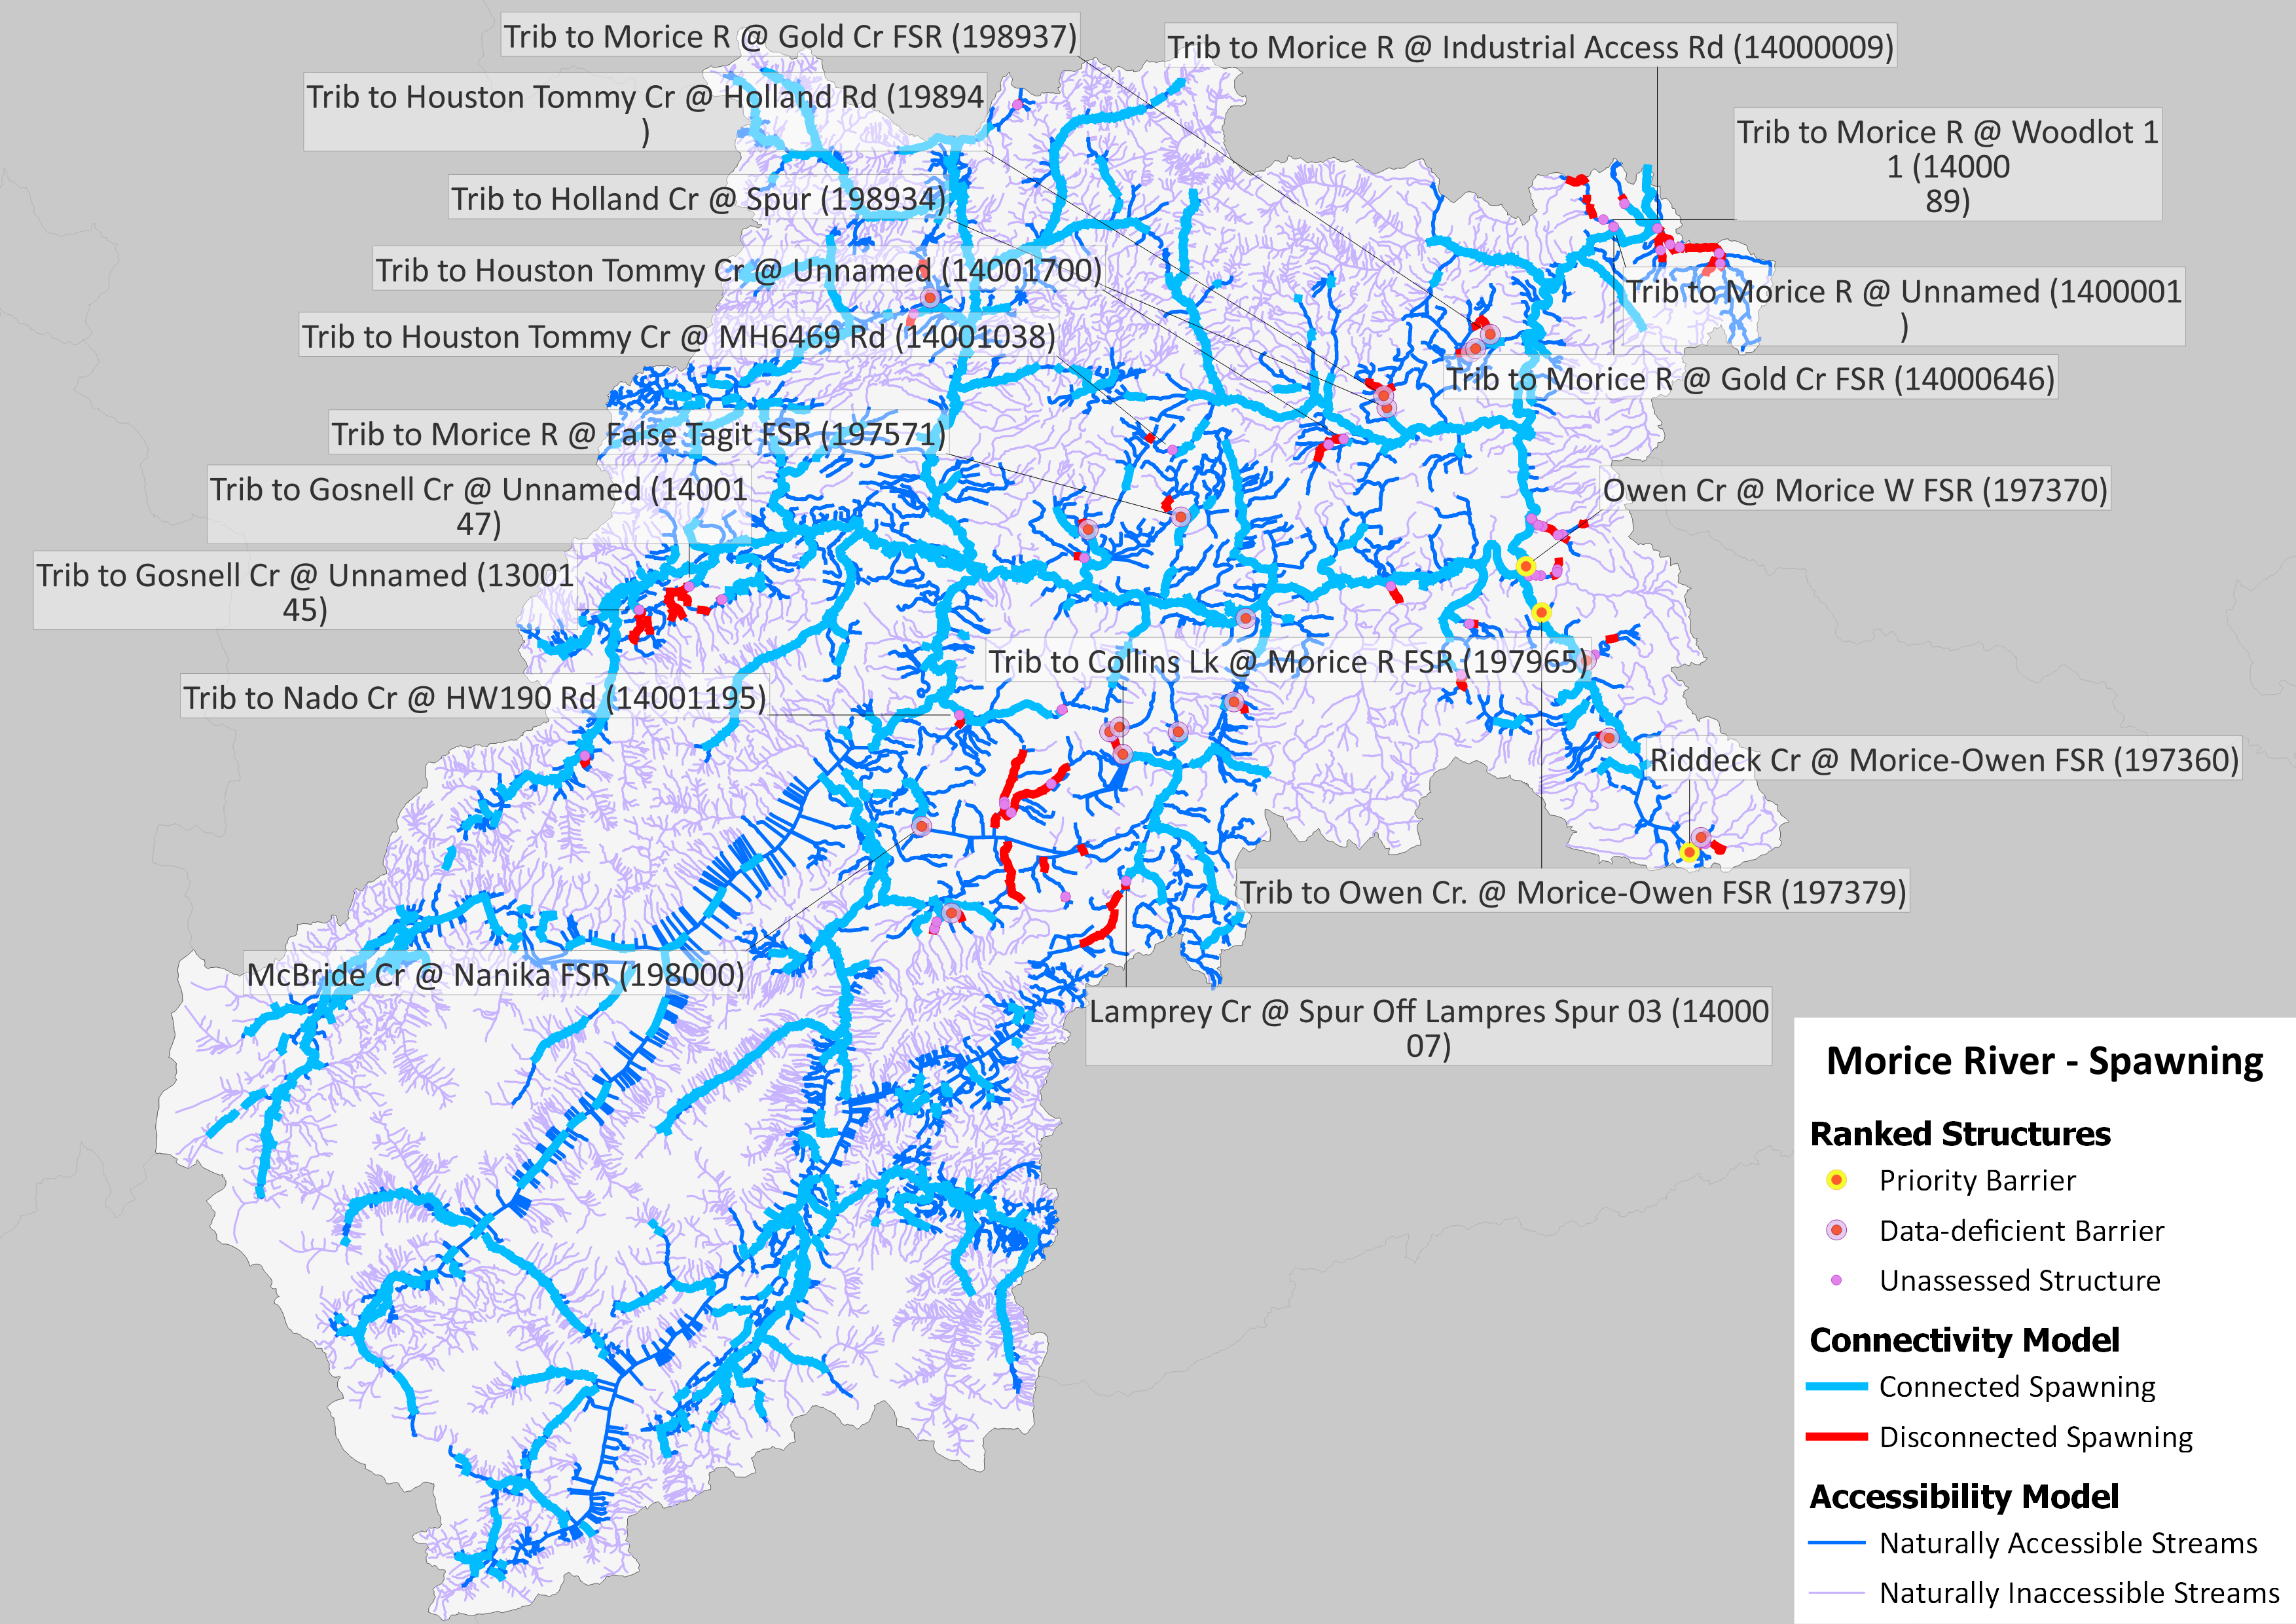
\includegraphics{content/images/Figure_1_Figure 5_spawning map.png}
\caption{Figure 5: Map of Pacific salmon and steelhead spawning habitat
and structures that are confirmed or potential barriers to fish passage
in the Morice River as of May 2026. Structure data were obtained from
BCFishPass and the Canadian Aquatic Barriers Database
(aquaticbarriers.ca). The accessibility model represents areas of the
watershed that one or more of Pacific salmon and steelhead could access
naturally in the absence of anthropogenic barriers. The habitat model
represents the subset of accessible waterbodies that may be used by one
or more Pacific salmon and steelhead for spawning. Available local
knowledge and data were incorporated and overruled habitat model
results. Thick red lines represent habitat considered to be fully
disconnected (upstream of barriers or unassessed structures)}
\end{figure}

\begin{figure}
\centering
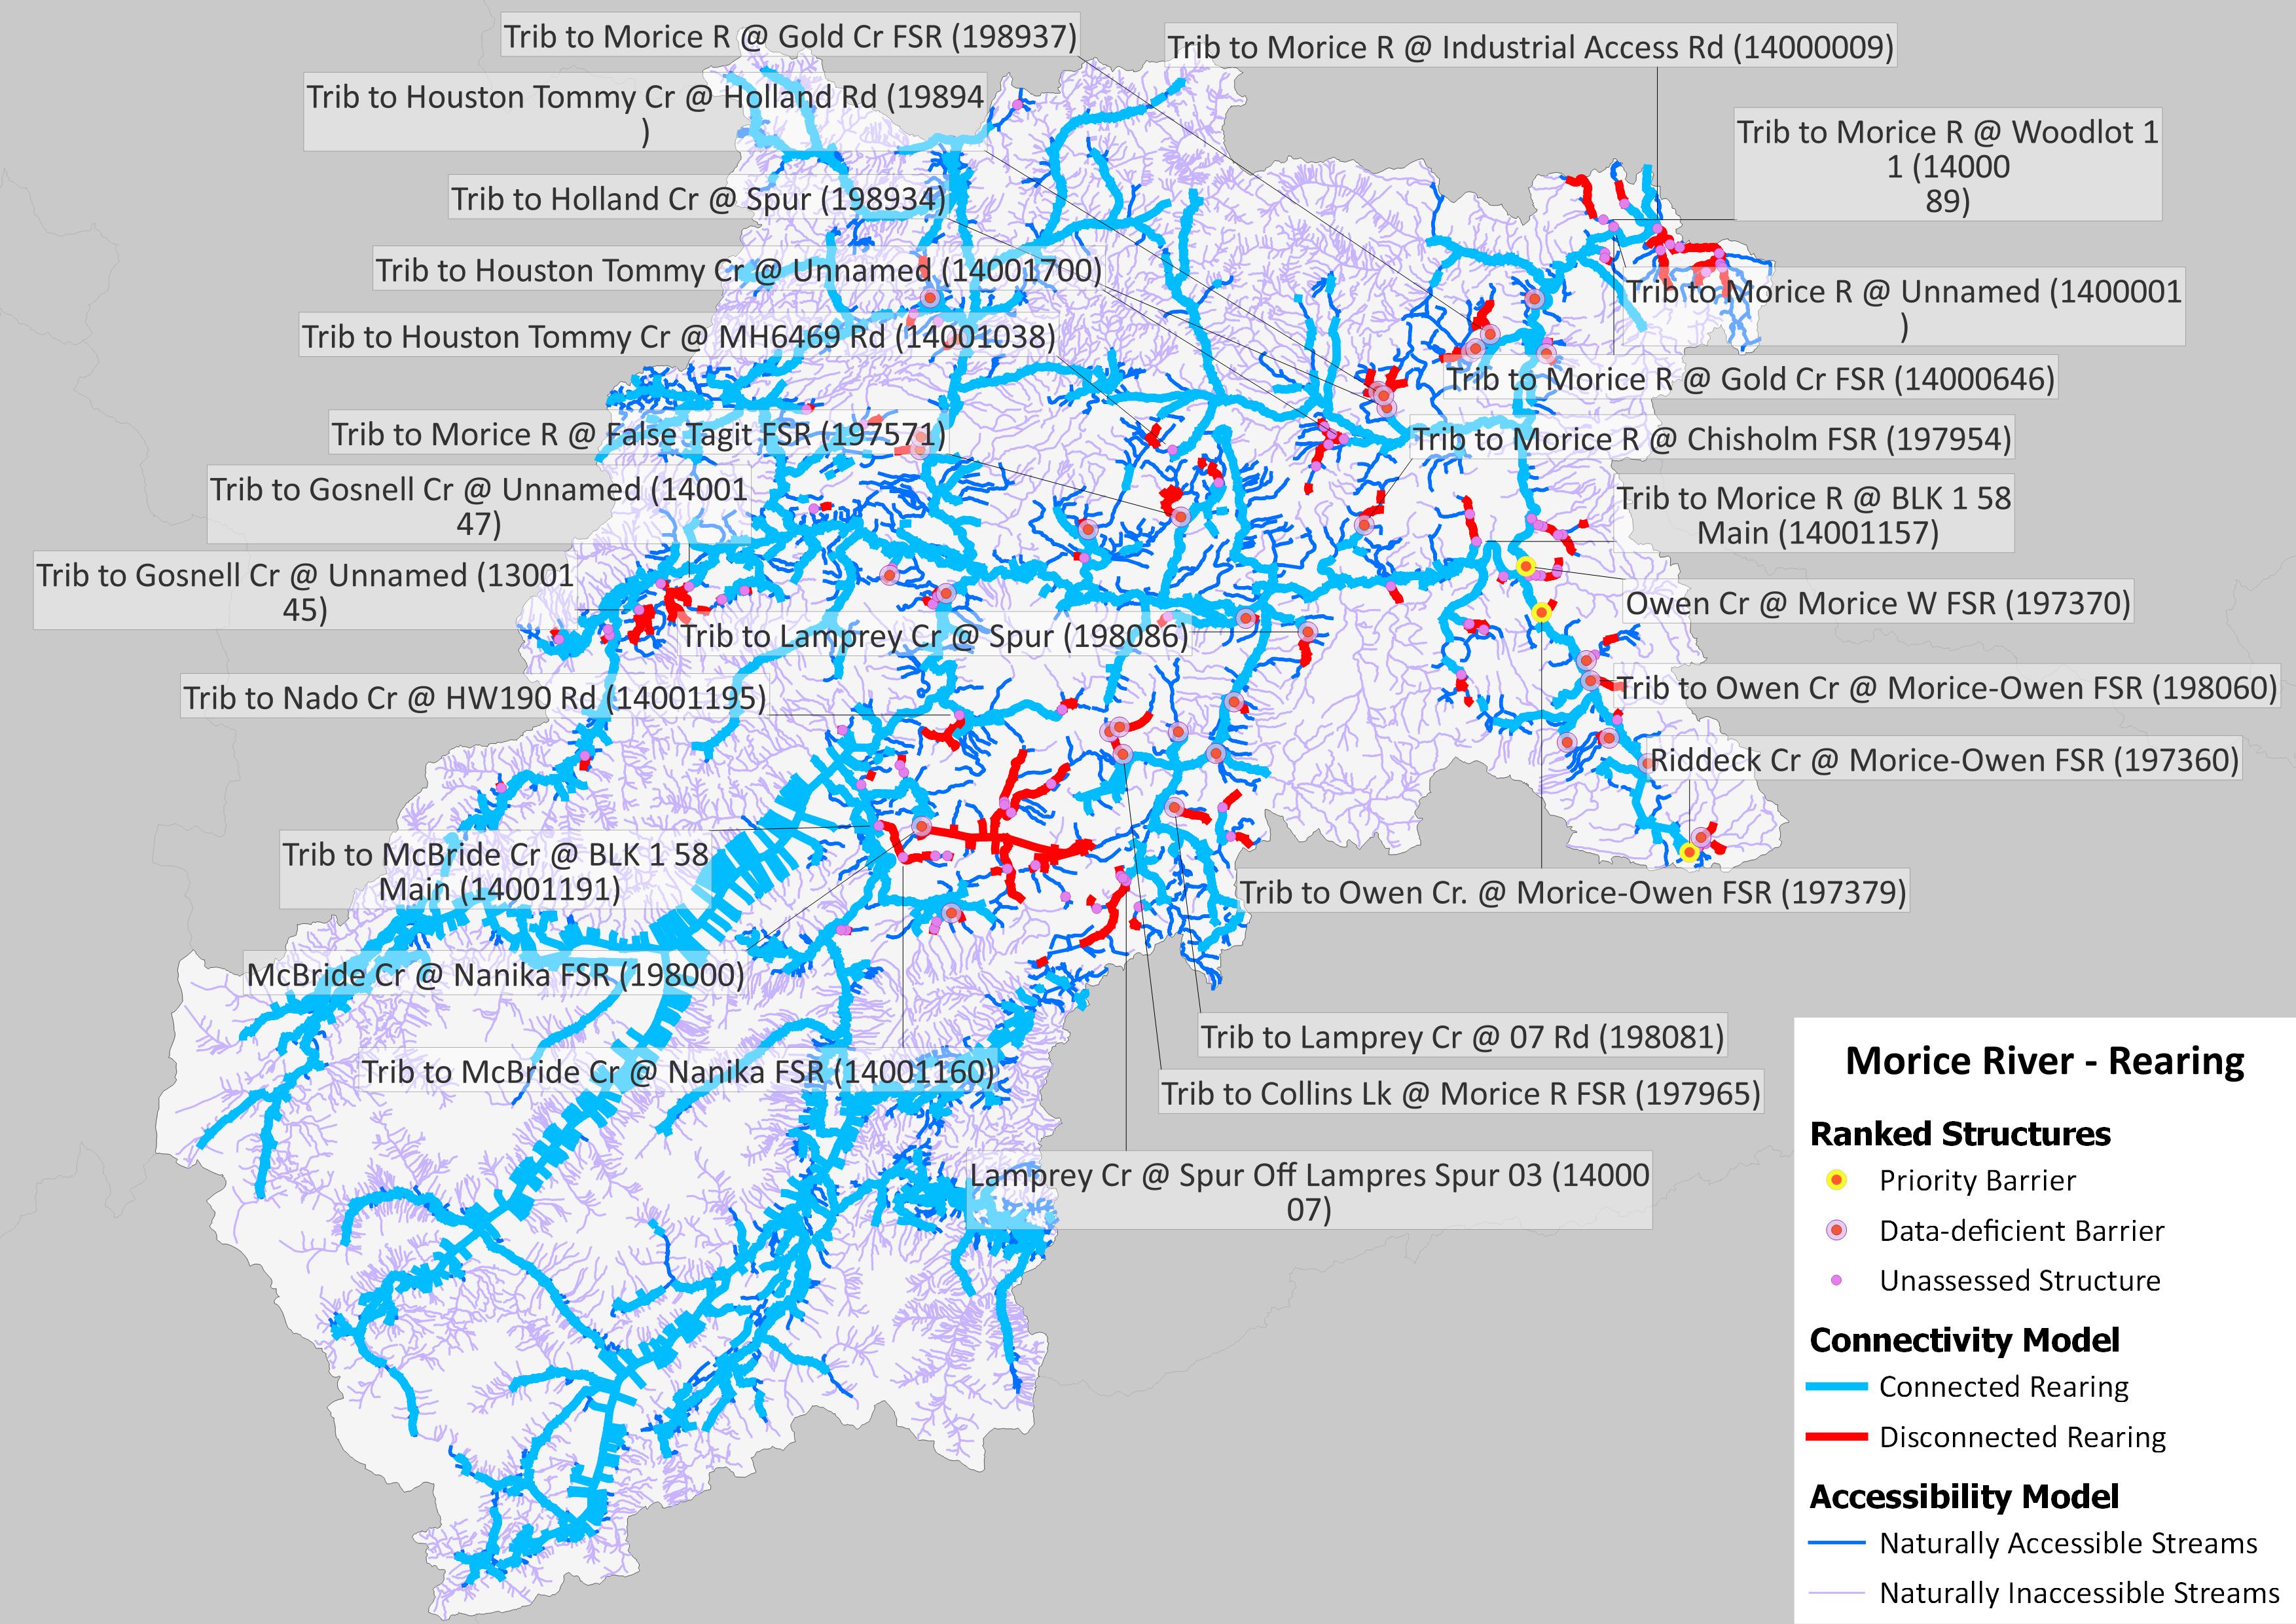
\includegraphics{content/images/Figure_2_Figure 6_rearing map.png}
\caption{Figure 6: Map of Pacific salmon and steelhead rearing habitat
and structures that are confirmed or potential barriers to fish passage
in the Morice River as of May 2026. Structure data were obtained from
BCFishPass and the Canadian Aquatic Barriers Database
(aquaticbarriers.ca). The accessibility model represents areas of the
watershed that one or more of Pacific salmon and steelhead could access
naturally in the absence of anthropogenic barriers. The habitat model
represents the subset of accessible waterbodies that may be used by one
or more Pacific salmon and steelhead for rearing. Available local
knowledge and data were incorporated and overruled habitat model
results. Thick red lines represent habitat considered to be fully
disconnected (upstream of barriers or unassessed structures)}
\end{figure}

\section*{Habitat Accumulation
Curves}\label{habitat-accumulation-curves}
\addcontentsline{toc}{section}{Habitat Accumulation Curves}

\markright{Habitat Accumulation Curves}

\begin{figure}
\centering
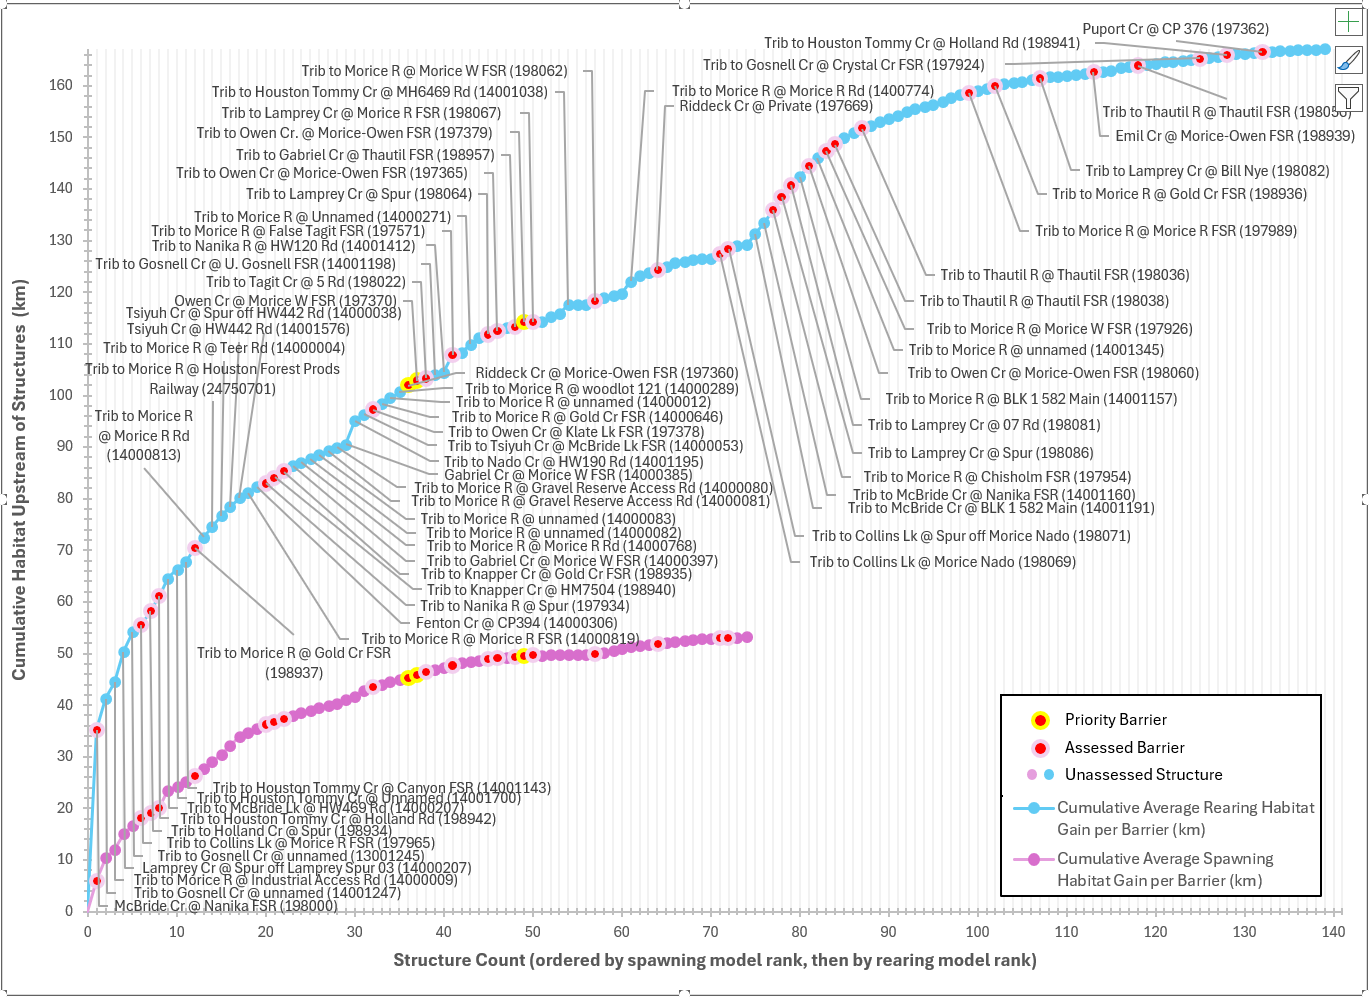
\includegraphics{content/images/Fig_3_Fig 7_MORR_HAC.png}
\caption{Figure 7: Habitat Accumulation Curve (HAC) showing structures
in the Morice River as of May 2026. Structures are ranked based on how
much (km) habitat for spawning and rearing habitat is upstream. The
y-axis represents the cumulative amount of potential habitat gain (km).
Sets of structures are indicated by a grey line below the curve,
indicating that gains from addressing the downstream structure alone
would be less than the combined gains from addressing all structures in
the set. Habitat upstream of unassessed structures is considered
disconnected until field assessments are completed. Structures that were
excluded as passable are not shown; however, rehabilitated barriers are
shown (where applicable) to demonstrate the connectivity gains achieved
through implementation of this plan.}
\end{figure}

\section*{Habitat Accumulation Summary
Table}\label{habitat-accumulation-summary-table}
\addcontentsline{toc}{section}{Habitat Accumulation Summary Table}

\markright{Habitat Accumulation Summary Table}

\global\setlength{\Oldarrayrulewidth}{\arrayrulewidth}

\global\setlength{\Oldtabcolsep}{\tabcolsep}

\setlength{\tabcolsep}{2pt}

\renewcommand*{\arraystretch}{1.5}



\providecommand{\ascline}[3]{\noalign{\global\arrayrulewidth #1}\arrayrulecolor[HTML]{#2}\cline{#3}}

\begin{longtable}[c]{|p{1.13in}|p{4.50in}|p{1.71in}|p{3.31in}|p{2.81in}|p{3.17in}|p{2.67in}}
\caption{Table 1: Labelled structures in the Habitat Accumulation Curve (Figure 3
and Figure 7), their rank, and upstream habitat for Pacific salmon and
steelhead in Morice River watershed. Habitat gain (averaged across sets)
represents the amount (km) of habitat upstream of that structure to the
next structure and depicts the potential gain in habitat if passage at
that structure was restored.}\tabularnewline




\hhline{>{\arrayrulecolor[HTML]{666666}\global\arrayrulewidth=1.5pt}->{\arrayrulecolor[HTML]{666666}\global\arrayrulewidth=1.5pt}->{\arrayrulecolor[HTML]{666666}\global\arrayrulewidth=1.5pt}->{\arrayrulecolor[HTML]{666666}\global\arrayrulewidth=1.5pt}->{\arrayrulecolor[HTML]{666666}\global\arrayrulewidth=1.5pt}->{\arrayrulecolor[HTML]{666666}\global\arrayrulewidth=1.5pt}->{\arrayrulecolor[HTML]{666666}\global\arrayrulewidth=1.5pt}-}

\multicolumn{1}{>{\cellcolor[HTML]{008270}\raggedright}m{\dimexpr 1.13in+0\tabcolsep}}{\textcolor[HTML]{FFFFFF}{\fontsize{11}{11}\selectfont{\global\setmainfont{Arial}{Barrier\ ID}}}} & \multicolumn{1}{>{\cellcolor[HTML]{008270}\raggedright}m{\dimexpr 4.5in+0\tabcolsep}}{\textcolor[HTML]{FFFFFF}{\fontsize{11}{11}\selectfont{\global\setmainfont{Arial}{Site\ Name}}}} & \multicolumn{1}{>{\cellcolor[HTML]{008270}\raggedright}m{\dimexpr 1.71in+0\tabcolsep}}{\textcolor[HTML]{FFFFFF}{\fontsize{11}{11}\selectfont{\global\setmainfont{Arial}{Structure\ Status}}}} & \multicolumn{1}{>{\cellcolor[HTML]{008270}\raggedright}m{\dimexpr 3.31in+0\tabcolsep}}{\textcolor[HTML]{FFFFFF}{\fontsize{11}{11}\selectfont{\global\setmainfont{Arial}{Rank\ Order\ (Spawning\ Habitat\ -\ All\ Species)}}}} & \multicolumn{1}{>{\cellcolor[HTML]{008270}\raggedright}m{\dimexpr 2.81in+0\tabcolsep}}{\textcolor[HTML]{FFFFFF}{\fontsize{11}{11}\selectfont{\global\setmainfont{Arial}{Average\ Spawning\ Habitat\ Gain\ (km)}}}} & \multicolumn{1}{>{\cellcolor[HTML]{008270}\raggedright}m{\dimexpr 3.17in+0\tabcolsep}}{\textcolor[HTML]{FFFFFF}{\fontsize{11}{11}\selectfont{\global\setmainfont{Arial}{Rank\ Order\ (Rearing\ Habitat\ -\ All\ Species)}}}} & \multicolumn{1}{>{\cellcolor[HTML]{008270}\raggedright}m{\dimexpr 2.67in+0\tabcolsep}}{\textcolor[HTML]{FFFFFF}{\fontsize{11}{11}\selectfont{\global\setmainfont{Arial}{Average\ Rearing\ Habitat\ Gain\ (km)}}}} \\

\noalign{\global\arrayrulewidth 0pt}\arrayrulecolor[HTML]{000000}

\hhline{>{\arrayrulecolor[HTML]{666666}\global\arrayrulewidth=1.5pt}->{\arrayrulecolor[HTML]{666666}\global\arrayrulewidth=1.5pt}->{\arrayrulecolor[HTML]{666666}\global\arrayrulewidth=1.5pt}->{\arrayrulecolor[HTML]{666666}\global\arrayrulewidth=1.5pt}->{\arrayrulecolor[HTML]{666666}\global\arrayrulewidth=1.5pt}->{\arrayrulecolor[HTML]{666666}\global\arrayrulewidth=1.5pt}->{\arrayrulecolor[HTML]{666666}\global\arrayrulewidth=1.5pt}-}\endfirsthead 

\hhline{>{\arrayrulecolor[HTML]{666666}\global\arrayrulewidth=1.5pt}->{\arrayrulecolor[HTML]{666666}\global\arrayrulewidth=1.5pt}->{\arrayrulecolor[HTML]{666666}\global\arrayrulewidth=1.5pt}->{\arrayrulecolor[HTML]{666666}\global\arrayrulewidth=1.5pt}->{\arrayrulecolor[HTML]{666666}\global\arrayrulewidth=1.5pt}->{\arrayrulecolor[HTML]{666666}\global\arrayrulewidth=1.5pt}->{\arrayrulecolor[HTML]{666666}\global\arrayrulewidth=1.5pt}-}

\multicolumn{1}{>{\cellcolor[HTML]{008270}\raggedright}m{\dimexpr 1.13in+0\tabcolsep}}{\textcolor[HTML]{FFFFFF}{\fontsize{11}{11}\selectfont{\global\setmainfont{Arial}{Barrier\ ID}}}} & \multicolumn{1}{>{\cellcolor[HTML]{008270}\raggedright}m{\dimexpr 4.5in+0\tabcolsep}}{\textcolor[HTML]{FFFFFF}{\fontsize{11}{11}\selectfont{\global\setmainfont{Arial}{Site\ Name}}}} & \multicolumn{1}{>{\cellcolor[HTML]{008270}\raggedright}m{\dimexpr 1.71in+0\tabcolsep}}{\textcolor[HTML]{FFFFFF}{\fontsize{11}{11}\selectfont{\global\setmainfont{Arial}{Structure\ Status}}}} & \multicolumn{1}{>{\cellcolor[HTML]{008270}\raggedright}m{\dimexpr 3.31in+0\tabcolsep}}{\textcolor[HTML]{FFFFFF}{\fontsize{11}{11}\selectfont{\global\setmainfont{Arial}{Rank\ Order\ (Spawning\ Habitat\ -\ All\ Species)}}}} & \multicolumn{1}{>{\cellcolor[HTML]{008270}\raggedright}m{\dimexpr 2.81in+0\tabcolsep}}{\textcolor[HTML]{FFFFFF}{\fontsize{11}{11}\selectfont{\global\setmainfont{Arial}{Average\ Spawning\ Habitat\ Gain\ (km)}}}} & \multicolumn{1}{>{\cellcolor[HTML]{008270}\raggedright}m{\dimexpr 3.17in+0\tabcolsep}}{\textcolor[HTML]{FFFFFF}{\fontsize{11}{11}\selectfont{\global\setmainfont{Arial}{Rank\ Order\ (Rearing\ Habitat\ -\ All\ Species)}}}} & \multicolumn{1}{>{\cellcolor[HTML]{008270}\raggedright}m{\dimexpr 2.67in+0\tabcolsep}}{\textcolor[HTML]{FFFFFF}{\fontsize{11}{11}\selectfont{\global\setmainfont{Arial}{Average\ Rearing\ Habitat\ Gain\ (km)}}}} \\

\noalign{\global\arrayrulewidth 0pt}\arrayrulecolor[HTML]{000000}

\hhline{>{\arrayrulecolor[HTML]{666666}\global\arrayrulewidth=1.5pt}->{\arrayrulecolor[HTML]{666666}\global\arrayrulewidth=1.5pt}->{\arrayrulecolor[HTML]{666666}\global\arrayrulewidth=1.5pt}->{\arrayrulecolor[HTML]{666666}\global\arrayrulewidth=1.5pt}->{\arrayrulecolor[HTML]{666666}\global\arrayrulewidth=1.5pt}->{\arrayrulecolor[HTML]{666666}\global\arrayrulewidth=1.5pt}->{\arrayrulecolor[HTML]{666666}\global\arrayrulewidth=1.5pt}-}\endhead



\multicolumn{1}{>{\raggedright}m{\dimexpr 1.13in+0\tabcolsep}}{\textcolor[HTML]{000000}{\fontsize{11}{11}\selectfont{\global\setmainfont{Arial}{198000}}}} & \multicolumn{1}{>{\raggedright}m{\dimexpr 4.5in+0\tabcolsep}}{\textcolor[HTML]{000000}{\fontsize{11}{11}\selectfont{\global\setmainfont{Arial}{McBride\ Cr\ @\ Nanika\ FSR\ (198000)}}}} & \multicolumn{1}{>{\raggedright}m{\dimexpr 1.71in+0\tabcolsep}}{\textcolor[HTML]{000000}{\fontsize{11}{11}\selectfont{\global\setmainfont{Arial}{Data-deficient\ barrier}}}} & \multicolumn{1}{>{\raggedright}m{\dimexpr 3.31in+0\tabcolsep}}{\textcolor[HTML]{000000}{\fontsize{11}{11}\selectfont{\global\setmainfont{Arial}{1}}}} & \multicolumn{1}{>{\raggedright}m{\dimexpr 2.81in+0\tabcolsep}}{\textcolor[HTML]{000000}{\fontsize{11}{11}\selectfont{\global\setmainfont{Arial}{5.95}}}} & \multicolumn{1}{>{\raggedright}m{\dimexpr 3.17in+0\tabcolsep}}{\textcolor[HTML]{000000}{\fontsize{11}{11}\selectfont{\global\setmainfont{Arial}{1}}}} & \multicolumn{1}{>{\raggedright}m{\dimexpr 2.67in+0\tabcolsep}}{\textcolor[HTML]{000000}{\fontsize{11}{11}\selectfont{\global\setmainfont{Arial}{35.21}}}} \\

\noalign{\global\arrayrulewidth 0pt}\arrayrulecolor[HTML]{000000}





\multicolumn{1}{>{\raggedright}m{\dimexpr 1.13in+0\tabcolsep}}{\textcolor[HTML]{000000}{\fontsize{11}{11}\selectfont{\global\setmainfont{Arial}{1014001247}}}} & \multicolumn{1}{>{\raggedright}m{\dimexpr 4.5in+0\tabcolsep}}{\textcolor[HTML]{000000}{\fontsize{11}{11}\selectfont{\global\setmainfont{Arial}{Trib\ to\ Gosnell\ Cr\ @\ unnamed\ (14001247)}}}} & \multicolumn{1}{>{\raggedright}m{\dimexpr 1.71in+0\tabcolsep}}{\textcolor[HTML]{000000}{\fontsize{11}{11}\selectfont{\global\setmainfont{Arial}{Unassessed}}}} & \multicolumn{1}{>{\raggedright}m{\dimexpr 3.31in+0\tabcolsep}}{\textcolor[HTML]{000000}{\fontsize{11}{11}\selectfont{\global\setmainfont{Arial}{2}}}} & \multicolumn{1}{>{\raggedright}m{\dimexpr 2.81in+0\tabcolsep}}{\textcolor[HTML]{000000}{\fontsize{11}{11}\selectfont{\global\setmainfont{Arial}{4.39}}}} & \multicolumn{1}{>{\raggedright}m{\dimexpr 3.17in+0\tabcolsep}}{\textcolor[HTML]{000000}{\fontsize{11}{11}\selectfont{\global\setmainfont{Arial}{3}}}} & \multicolumn{1}{>{\raggedright}m{\dimexpr 2.67in+0\tabcolsep}}{\textcolor[HTML]{000000}{\fontsize{11}{11}\selectfont{\global\setmainfont{Arial}{6.04}}}} \\

\noalign{\global\arrayrulewidth 0pt}\arrayrulecolor[HTML]{000000}





\multicolumn{1}{>{\raggedright}m{\dimexpr 1.13in+0\tabcolsep}}{\textcolor[HTML]{000000}{\fontsize{11}{11}\selectfont{\global\setmainfont{Arial}{1014000009}}}} & \multicolumn{1}{>{\raggedright}m{\dimexpr 4.5in+0\tabcolsep}}{\textcolor[HTML]{000000}{\fontsize{11}{11}\selectfont{\global\setmainfont{Arial}{Trib\ to\ Morice\ R\ @\ Industrial\ Access\ Rd\ (14000009)}}}} & \multicolumn{1}{>{\raggedright}m{\dimexpr 1.71in+0\tabcolsep}}{\textcolor[HTML]{000000}{\fontsize{11}{11}\selectfont{\global\setmainfont{Arial}{Unassessed}}}} & \multicolumn{1}{>{\raggedright}m{\dimexpr 3.31in+0\tabcolsep}}{\textcolor[HTML]{000000}{\fontsize{11}{11}\selectfont{\global\setmainfont{Arial}{3}}}} & \multicolumn{1}{>{\raggedright}m{\dimexpr 2.81in+0\tabcolsep}}{\textcolor[HTML]{000000}{\fontsize{11}{11}\selectfont{\global\setmainfont{Arial}{1.62}}}} & \multicolumn{1}{>{\raggedright}m{\dimexpr 3.17in+0\tabcolsep}}{\textcolor[HTML]{000000}{\fontsize{11}{11}\selectfont{\global\setmainfont{Arial}{4}}}} & \multicolumn{1}{>{\raggedright}m{\dimexpr 2.67in+0\tabcolsep}}{\textcolor[HTML]{000000}{\fontsize{11}{11}\selectfont{\global\setmainfont{Arial}{3.19}}}} \\

\noalign{\global\arrayrulewidth 0pt}\arrayrulecolor[HTML]{000000}





\multicolumn{1}{>{\raggedright}m{\dimexpr 1.13in+0\tabcolsep}}{\textcolor[HTML]{000000}{\fontsize{11}{11}\selectfont{\global\setmainfont{Arial}{1014000207}}}} & \multicolumn{1}{>{\raggedright}m{\dimexpr 4.5in+0\tabcolsep}}{\textcolor[HTML]{000000}{\fontsize{11}{11}\selectfont{\global\setmainfont{Arial}{Lamprey\ Cr\ @\ Spur\ off\ Lamprey\ Spur\ 03\ (14000207)}}}} & \multicolumn{1}{>{\raggedright}m{\dimexpr 1.71in+0\tabcolsep}}{\textcolor[HTML]{000000}{\fontsize{11}{11}\selectfont{\global\setmainfont{Arial}{Unassessed}}}} & \multicolumn{1}{>{\raggedright}m{\dimexpr 3.31in+0\tabcolsep}}{\textcolor[HTML]{000000}{\fontsize{11}{11}\selectfont{\global\setmainfont{Arial}{4}}}} & \multicolumn{1}{>{\raggedright}m{\dimexpr 2.81in+0\tabcolsep}}{\textcolor[HTML]{000000}{\fontsize{11}{11}\selectfont{\global\setmainfont{Arial}{3.05}}}} & \multicolumn{1}{>{\raggedright}m{\dimexpr 3.17in+0\tabcolsep}}{\textcolor[HTML]{000000}{\fontsize{11}{11}\selectfont{\global\setmainfont{Arial}{2}}}} & \multicolumn{1}{>{\raggedright}m{\dimexpr 2.67in+0\tabcolsep}}{\textcolor[HTML]{000000}{\fontsize{11}{11}\selectfont{\global\setmainfont{Arial}{5.89}}}} \\

\noalign{\global\arrayrulewidth 0pt}\arrayrulecolor[HTML]{000000}





\multicolumn{1}{>{\raggedright}m{\dimexpr 1.13in+0\tabcolsep}}{\textcolor[HTML]{000000}{\fontsize{11}{11}\selectfont{\global\setmainfont{Arial}{1014001245}}}} & \multicolumn{1}{>{\raggedright}m{\dimexpr 4.5in+0\tabcolsep}}{\textcolor[HTML]{000000}{\fontsize{11}{11}\selectfont{\global\setmainfont{Arial}{Trib\ to\ Gosnell\ Cr\ @\ unnamed\ (13001245)}}}} & \multicolumn{1}{>{\raggedright}m{\dimexpr 1.71in+0\tabcolsep}}{\textcolor[HTML]{000000}{\fontsize{11}{11}\selectfont{\global\setmainfont{Arial}{Unassessed}}}} & \multicolumn{1}{>{\raggedright}m{\dimexpr 3.31in+0\tabcolsep}}{\textcolor[HTML]{000000}{\fontsize{11}{11}\selectfont{\global\setmainfont{Arial}{5}}}} & \multicolumn{1}{>{\raggedright}m{\dimexpr 2.81in+0\tabcolsep}}{\textcolor[HTML]{000000}{\fontsize{11}{11}\selectfont{\global\setmainfont{Arial}{1.75}}}} & \multicolumn{1}{>{\raggedright}m{\dimexpr 3.17in+0\tabcolsep}}{\textcolor[HTML]{000000}{\fontsize{11}{11}\selectfont{\global\setmainfont{Arial}{7}}}} & \multicolumn{1}{>{\raggedright}m{\dimexpr 2.67in+0\tabcolsep}}{\textcolor[HTML]{000000}{\fontsize{11}{11}\selectfont{\global\setmainfont{Arial}{3.81}}}} \\

\noalign{\global\arrayrulewidth 0pt}\arrayrulecolor[HTML]{000000}





\multicolumn{1}{>{\raggedright}m{\dimexpr 1.13in+0\tabcolsep}}{\textcolor[HTML]{000000}{\fontsize{11}{11}\selectfont{\global\setmainfont{Arial}{197965}}}} & \multicolumn{1}{>{\raggedright}m{\dimexpr 4.5in+0\tabcolsep}}{\textcolor[HTML]{000000}{\fontsize{11}{11}\selectfont{\global\setmainfont{Arial}{Trib\ to\ Collins\ Lk\ @\ Morice\ R\ FSR\ (197965)}}}} & \multicolumn{1}{>{\raggedright}m{\dimexpr 1.71in+0\tabcolsep}}{\textcolor[HTML]{000000}{\fontsize{11}{11}\selectfont{\global\setmainfont{Arial}{Data-deficient\ barrier}}}} & \multicolumn{1}{>{\raggedright}m{\dimexpr 3.31in+0\tabcolsep}}{\textcolor[HTML]{000000}{\fontsize{11}{11}\selectfont{\global\setmainfont{Arial}{6}}}} & \multicolumn{1}{>{\raggedright}m{\dimexpr 2.81in+0\tabcolsep}}{\textcolor[HTML]{000000}{\fontsize{11}{11}\selectfont{\global\setmainfont{Arial}{1.35}}}} & \multicolumn{1}{>{\raggedright}m{\dimexpr 3.17in+0\tabcolsep}}{\textcolor[HTML]{000000}{\fontsize{11}{11}\selectfont{\global\setmainfont{Arial}{12}}}} & \multicolumn{1}{>{\raggedright}m{\dimexpr 2.67in+0\tabcolsep}}{\textcolor[HTML]{000000}{\fontsize{11}{11}\selectfont{\global\setmainfont{Arial}{1.36}}}} \\

\noalign{\global\arrayrulewidth 0pt}\arrayrulecolor[HTML]{000000}





\multicolumn{1}{>{\raggedright}m{\dimexpr 1.13in+0\tabcolsep}}{\textcolor[HTML]{000000}{\fontsize{11}{11}\selectfont{\global\setmainfont{Arial}{198934}}}} & \multicolumn{1}{>{\raggedright}m{\dimexpr 4.5in+0\tabcolsep}}{\textcolor[HTML]{000000}{\fontsize{11}{11}\selectfont{\global\setmainfont{Arial}{Trib\ to\ Holland\ Cr\ @\ Spur\ (198934)}}}} & \multicolumn{1}{>{\raggedright}m{\dimexpr 1.71in+0\tabcolsep}}{\textcolor[HTML]{000000}{\fontsize{11}{11}\selectfont{\global\setmainfont{Arial}{Data-deficient\ barrier}}}} & \multicolumn{1}{>{\raggedright}m{\dimexpr 3.31in+0\tabcolsep}}{\textcolor[HTML]{000000}{\fontsize{11}{11}\selectfont{\global\setmainfont{Arial}{7}}}} & \multicolumn{1}{>{\raggedright}m{\dimexpr 2.81in+0\tabcolsep}}{\textcolor[HTML]{000000}{\fontsize{11}{11}\selectfont{\global\setmainfont{Arial}{0.98}}}} & \multicolumn{1}{>{\raggedright}m{\dimexpr 3.17in+0\tabcolsep}}{\textcolor[HTML]{000000}{\fontsize{11}{11}\selectfont{\global\setmainfont{Arial}{6}}}} & \multicolumn{1}{>{\raggedright}m{\dimexpr 2.67in+0\tabcolsep}}{\textcolor[HTML]{000000}{\fontsize{11}{11}\selectfont{\global\setmainfont{Arial}{2.79}}}} \\

\noalign{\global\arrayrulewidth 0pt}\arrayrulecolor[HTML]{000000}





\multicolumn{1}{>{\raggedright}m{\dimexpr 1.13in+0\tabcolsep}}{\textcolor[HTML]{000000}{\fontsize{11}{11}\selectfont{\global\setmainfont{Arial}{198942}}}} & \multicolumn{1}{>{\raggedright}m{\dimexpr 4.5in+0\tabcolsep}}{\textcolor[HTML]{000000}{\fontsize{11}{11}\selectfont{\global\setmainfont{Arial}{Trib\ to\ Houston\ Tommy\ Cr\ @\ Holland\ Rd\ (198942)}}}} & \multicolumn{1}{>{\raggedright}m{\dimexpr 1.71in+0\tabcolsep}}{\textcolor[HTML]{000000}{\fontsize{11}{11}\selectfont{\global\setmainfont{Arial}{Data-deficient\ barrier}}}} & \multicolumn{1}{>{\raggedright}m{\dimexpr 3.31in+0\tabcolsep}}{\textcolor[HTML]{000000}{\fontsize{11}{11}\selectfont{\global\setmainfont{Arial}{7}}}} & \multicolumn{1}{>{\raggedright}m{\dimexpr 2.81in+0\tabcolsep}}{\textcolor[HTML]{000000}{\fontsize{11}{11}\selectfont{\global\setmainfont{Arial}{0.98}}}} & \multicolumn{1}{>{\raggedright}m{\dimexpr 3.17in+0\tabcolsep}}{\textcolor[HTML]{000000}{\fontsize{11}{11}\selectfont{\global\setmainfont{Arial}{6}}}} & \multicolumn{1}{>{\raggedright}m{\dimexpr 2.67in+0\tabcolsep}}{\textcolor[HTML]{000000}{\fontsize{11}{11}\selectfont{\global\setmainfont{Arial}{2.79}}}} \\

\noalign{\global\arrayrulewidth 0pt}\arrayrulecolor[HTML]{000000}





\multicolumn{1}{>{\raggedright}m{\dimexpr 1.13in+0\tabcolsep}}{\textcolor[HTML]{000000}{\fontsize{11}{11}\selectfont{\global\setmainfont{Arial}{1014000040}}}} & \multicolumn{1}{>{\raggedright}m{\dimexpr 4.5in+0\tabcolsep}}{\textcolor[HTML]{000000}{\fontsize{11}{11}\selectfont{\global\setmainfont{Arial}{Trib\ to\ McBride\ Lk\ @\ HW469\ Rd\ (14000207)}}}} & \multicolumn{1}{>{\raggedright}m{\dimexpr 1.71in+0\tabcolsep}}{\textcolor[HTML]{000000}{\fontsize{11}{11}\selectfont{\global\setmainfont{Arial}{Unassessed}}}} & \multicolumn{1}{>{\raggedright}m{\dimexpr 3.31in+0\tabcolsep}}{\textcolor[HTML]{000000}{\fontsize{11}{11}\selectfont{\global\setmainfont{Arial}{8}}}} & \multicolumn{1}{>{\raggedright}m{\dimexpr 2.81in+0\tabcolsep}}{\textcolor[HTML]{000000}{\fontsize{11}{11}\selectfont{\global\setmainfont{Arial}{3.40}}}} & \multicolumn{1}{>{\raggedright}m{\dimexpr 3.17in+0\tabcolsep}}{\textcolor[HTML]{000000}{\fontsize{11}{11}\selectfont{\global\setmainfont{Arial}{28}}}} & \multicolumn{1}{>{\raggedright}m{\dimexpr 2.67in+0\tabcolsep}}{\textcolor[HTML]{000000}{\fontsize{11}{11}\selectfont{\global\setmainfont{Arial}{3.40}}}} \\

\noalign{\global\arrayrulewidth 0pt}\arrayrulecolor[HTML]{000000}





\multicolumn{1}{>{\raggedright}m{\dimexpr 1.13in+0\tabcolsep}}{\textcolor[HTML]{000000}{\fontsize{11}{11}\selectfont{\global\setmainfont{Arial}{1014001700}}}} & \multicolumn{1}{>{\raggedright}m{\dimexpr 4.5in+0\tabcolsep}}{\textcolor[HTML]{000000}{\fontsize{11}{11}\selectfont{\global\setmainfont{Arial}{Trib\ to\ Houston\ Tommy\ Cr\ @\ Unnamed\ (14001700)}}}} & \multicolumn{1}{>{\raggedright}m{\dimexpr 1.71in+0\tabcolsep}}{\textcolor[HTML]{000000}{\fontsize{11}{11}\selectfont{\global\setmainfont{Arial}{Unassessed}}}} & \multicolumn{1}{>{\raggedright}m{\dimexpr 3.31in+0\tabcolsep}}{\textcolor[HTML]{000000}{\fontsize{11}{11}\selectfont{\global\setmainfont{Arial}{9}}}} & \multicolumn{1}{>{\raggedright}m{\dimexpr 2.81in+0\tabcolsep}}{\textcolor[HTML]{000000}{\fontsize{11}{11}\selectfont{\global\setmainfont{Arial}{0.78}}}} & \multicolumn{1}{>{\raggedright}m{\dimexpr 3.17in+0\tabcolsep}}{\textcolor[HTML]{000000}{\fontsize{11}{11}\selectfont{\global\setmainfont{Arial}{10}}}} & \multicolumn{1}{>{\raggedright}m{\dimexpr 2.67in+0\tabcolsep}}{\textcolor[HTML]{000000}{\fontsize{11}{11}\selectfont{\global\setmainfont{Arial}{1.80}}}} \\

\noalign{\global\arrayrulewidth 0pt}\arrayrulecolor[HTML]{000000}





\multicolumn{1}{>{\raggedright}m{\dimexpr 1.13in+0\tabcolsep}}{\textcolor[HTML]{000000}{\fontsize{11}{11}\selectfont{\global\setmainfont{Arial}{1014001143}}}} & \multicolumn{1}{>{\raggedright}m{\dimexpr 4.5in+0\tabcolsep}}{\textcolor[HTML]{000000}{\fontsize{11}{11}\selectfont{\global\setmainfont{Arial}{Trib\ to\ Houston\ Tommy\ Cr\ @\ Canyon\ FSR\ (14001143)}}}} & \multicolumn{1}{>{\raggedright}m{\dimexpr 1.71in+0\tabcolsep}}{\textcolor[HTML]{000000}{\fontsize{11}{11}\selectfont{\global\setmainfont{Arial}{Unassessed}}}} & \multicolumn{1}{>{\raggedright}m{\dimexpr 3.31in+0\tabcolsep}}{\textcolor[HTML]{000000}{\fontsize{11}{11}\selectfont{\global\setmainfont{Arial}{9}}}} & \multicolumn{1}{>{\raggedright}m{\dimexpr 2.81in+0\tabcolsep}}{\textcolor[HTML]{000000}{\fontsize{11}{11}\selectfont{\global\setmainfont{Arial}{0.78}}}} & \multicolumn{1}{>{\raggedright}m{\dimexpr 3.17in+0\tabcolsep}}{\textcolor[HTML]{000000}{\fontsize{11}{11}\selectfont{\global\setmainfont{Arial}{45}}}} & \multicolumn{1}{>{\raggedright}m{\dimexpr 2.67in+0\tabcolsep}}{\textcolor[HTML]{000000}{\fontsize{11}{11}\selectfont{\global\setmainfont{Arial}{1.42}}}} \\

\noalign{\global\arrayrulewidth 0pt}\arrayrulecolor[HTML]{000000}





\multicolumn{1}{>{\raggedright}m{\dimexpr 1.13in+0\tabcolsep}}{\textcolor[HTML]{000000}{\fontsize{11}{11}\selectfont{\global\setmainfont{Arial}{198937}}}} & \multicolumn{1}{>{\raggedright}m{\dimexpr 4.5in+0\tabcolsep}}{\textcolor[HTML]{000000}{\fontsize{11}{11}\selectfont{\global\setmainfont{Arial}{Trib\ to\ Morice\ R\ @\ Gold\ Cr\ FSR\ (198937)}}}} & \multicolumn{1}{>{\raggedright}m{\dimexpr 1.71in+0\tabcolsep}}{\textcolor[HTML]{000000}{\fontsize{11}{11}\selectfont{\global\setmainfont{Arial}{Data-deficient\ barrier}}}} & \multicolumn{1}{>{\raggedright}m{\dimexpr 3.31in+0\tabcolsep}}{\textcolor[HTML]{000000}{\fontsize{11}{11}\selectfont{\global\setmainfont{Arial}{10}}}} & \multicolumn{1}{>{\raggedright}m{\dimexpr 2.81in+0\tabcolsep}}{\textcolor[HTML]{000000}{\fontsize{11}{11}\selectfont{\global\setmainfont{Arial}{1.15}}}} & \multicolumn{1}{>{\raggedright}m{\dimexpr 3.17in+0\tabcolsep}}{\textcolor[HTML]{000000}{\fontsize{11}{11}\selectfont{\global\setmainfont{Arial}{11}}}} & \multicolumn{1}{>{\raggedright}m{\dimexpr 2.67in+0\tabcolsep}}{\textcolor[HTML]{000000}{\fontsize{11}{11}\selectfont{\global\setmainfont{Arial}{2.72}}}} \\

\noalign{\global\arrayrulewidth 0pt}\arrayrulecolor[HTML]{000000}





\multicolumn{1}{>{\raggedright}m{\dimexpr 1.13in+0\tabcolsep}}{\textcolor[HTML]{000000}{\fontsize{11}{11}\selectfont{\global\setmainfont{Arial}{1014000813}}}} & \multicolumn{1}{>{\raggedright}m{\dimexpr 4.5in+0\tabcolsep}}{\textcolor[HTML]{000000}{\fontsize{11}{11}\selectfont{\global\setmainfont{Arial}{Trib\ to\ Morice\ R\ @\ Morice\ R\ Rd\ (14000813)}}}} & \multicolumn{1}{>{\raggedright}m{\dimexpr 1.71in+0\tabcolsep}}{\textcolor[HTML]{000000}{\fontsize{11}{11}\selectfont{\global\setmainfont{Arial}{Unassessed}}}} & \multicolumn{1}{>{\raggedright}m{\dimexpr 3.31in+0\tabcolsep}}{\textcolor[HTML]{000000}{\fontsize{11}{11}\selectfont{\global\setmainfont{Arial}{11}}}} & \multicolumn{1}{>{\raggedright}m{\dimexpr 2.81in+0\tabcolsep}}{\textcolor[HTML]{000000}{\fontsize{11}{11}\selectfont{\global\setmainfont{Arial}{1.41}}}} & \multicolumn{1}{>{\raggedright}m{\dimexpr 3.17in+0\tabcolsep}}{\textcolor[HTML]{000000}{\fontsize{11}{11}\selectfont{\global\setmainfont{Arial}{27}}}} & \multicolumn{1}{>{\raggedright}m{\dimexpr 2.67in+0\tabcolsep}}{\textcolor[HTML]{000000}{\fontsize{11}{11}\selectfont{\global\setmainfont{Arial}{2.09}}}} \\

\noalign{\global\arrayrulewidth 0pt}\arrayrulecolor[HTML]{000000}





\multicolumn{1}{>{\raggedright}m{\dimexpr 1.13in+0\tabcolsep}}{\textcolor[HTML]{000000}{\fontsize{11}{11}\selectfont{\global\setmainfont{Arial}{1024750701}}}} & \multicolumn{1}{>{\raggedright}m{\dimexpr 4.5in+0\tabcolsep}}{\textcolor[HTML]{000000}{\fontsize{11}{11}\selectfont{\global\setmainfont{Arial}{Trib\ to\ Morice\ R\ @\ Houston\ Forest\ Prods\ Railway\ (24750701)}}}} & \multicolumn{1}{>{\raggedright}m{\dimexpr 1.71in+0\tabcolsep}}{\textcolor[HTML]{000000}{\fontsize{11}{11}\selectfont{\global\setmainfont{Arial}{Unassessed}}}} & \multicolumn{1}{>{\raggedright}m{\dimexpr 3.31in+0\tabcolsep}}{\textcolor[HTML]{000000}{\fontsize{11}{11}\selectfont{\global\setmainfont{Arial}{11}}}} & \multicolumn{1}{>{\raggedright}m{\dimexpr 2.81in+0\tabcolsep}}{\textcolor[HTML]{000000}{\fontsize{11}{11}\selectfont{\global\setmainfont{Arial}{1.41}}}} & \multicolumn{1}{>{\raggedright}m{\dimexpr 3.17in+0\tabcolsep}}{\textcolor[HTML]{000000}{\fontsize{11}{11}\selectfont{\global\setmainfont{Arial}{27}}}} & \multicolumn{1}{>{\raggedright}m{\dimexpr 2.67in+0\tabcolsep}}{\textcolor[HTML]{000000}{\fontsize{11}{11}\selectfont{\global\setmainfont{Arial}{2.09}}}} \\

\noalign{\global\arrayrulewidth 0pt}\arrayrulecolor[HTML]{000000}





\multicolumn{1}{>{\raggedright}m{\dimexpr 1.13in+0\tabcolsep}}{\textcolor[HTML]{000000}{\fontsize{11}{11}\selectfont{\global\setmainfont{Arial}{1014000004}}}} & \multicolumn{1}{>{\raggedright}m{\dimexpr 4.5in+0\tabcolsep}}{\textcolor[HTML]{000000}{\fontsize{11}{11}\selectfont{\global\setmainfont{Arial}{Trib\ to\ Morice\ R\ @\ Teer\ Rd\ (14000004)}}}} & \multicolumn{1}{>{\raggedright}m{\dimexpr 1.71in+0\tabcolsep}}{\textcolor[HTML]{000000}{\fontsize{11}{11}\selectfont{\global\setmainfont{Arial}{Unassessed}}}} & \multicolumn{1}{>{\raggedright}m{\dimexpr 3.31in+0\tabcolsep}}{\textcolor[HTML]{000000}{\fontsize{11}{11}\selectfont{\global\setmainfont{Arial}{11}}}} & \multicolumn{1}{>{\raggedright}m{\dimexpr 2.81in+0\tabcolsep}}{\textcolor[HTML]{000000}{\fontsize{11}{11}\selectfont{\global\setmainfont{Arial}{1.41}}}} & \multicolumn{1}{>{\raggedright}m{\dimexpr 3.17in+0\tabcolsep}}{\textcolor[HTML]{000000}{\fontsize{11}{11}\selectfont{\global\setmainfont{Arial}{27}}}} & \multicolumn{1}{>{\raggedright}m{\dimexpr 2.67in+0\tabcolsep}}{\textcolor[HTML]{000000}{\fontsize{11}{11}\selectfont{\global\setmainfont{Arial}{2.09}}}} \\

\noalign{\global\arrayrulewidth 0pt}\arrayrulecolor[HTML]{000000}





\multicolumn{1}{>{\raggedright}m{\dimexpr 1.13in+0\tabcolsep}}{\textcolor[HTML]{000000}{\fontsize{11}{11}\selectfont{\global\setmainfont{Arial}{1014001576}}}} & \multicolumn{1}{>{\raggedright}m{\dimexpr 4.5in+0\tabcolsep}}{\textcolor[HTML]{000000}{\fontsize{11}{11}\selectfont{\global\setmainfont{Arial}{Tsiyuh\ Cr\ @\ HW442\ Rd\ (14001576)}}}} & \multicolumn{1}{>{\raggedright}m{\dimexpr 1.71in+0\tabcolsep}}{\textcolor[HTML]{000000}{\fontsize{11}{11}\selectfont{\global\setmainfont{Arial}{Unassessed}}}} & \multicolumn{1}{>{\raggedright}m{\dimexpr 3.31in+0\tabcolsep}}{\textcolor[HTML]{000000}{\fontsize{11}{11}\selectfont{\global\setmainfont{Arial}{12}}}} & \multicolumn{1}{>{\raggedright}m{\dimexpr 2.81in+0\tabcolsep}}{\textcolor[HTML]{000000}{\fontsize{11}{11}\selectfont{\global\setmainfont{Arial}{1.73}}}} & \multicolumn{1}{>{\raggedright}m{\dimexpr 3.17in+0\tabcolsep}}{\textcolor[HTML]{000000}{\fontsize{11}{11}\selectfont{\global\setmainfont{Arial}{33}}}} & \multicolumn{1}{>{\raggedright}m{\dimexpr 2.67in+0\tabcolsep}}{\textcolor[HTML]{000000}{\fontsize{11}{11}\selectfont{\global\setmainfont{Arial}{1.73}}}} \\

\noalign{\global\arrayrulewidth 0pt}\arrayrulecolor[HTML]{000000}





\multicolumn{1}{>{\raggedright}m{\dimexpr 1.13in+0\tabcolsep}}{\textcolor[HTML]{000000}{\fontsize{11}{11}\selectfont{\global\setmainfont{Arial}{1014000038}}}} & \multicolumn{1}{>{\raggedright}m{\dimexpr 4.5in+0\tabcolsep}}{\textcolor[HTML]{000000}{\fontsize{11}{11}\selectfont{\global\setmainfont{Arial}{Tsiyuh\ Cr\ @\ Spur\ off\ HW442\ Rd\ (14000038)}}}} & \multicolumn{1}{>{\raggedright}m{\dimexpr 1.71in+0\tabcolsep}}{\textcolor[HTML]{000000}{\fontsize{11}{11}\selectfont{\global\setmainfont{Arial}{Unassessed}}}} & \multicolumn{1}{>{\raggedright}m{\dimexpr 3.31in+0\tabcolsep}}{\textcolor[HTML]{000000}{\fontsize{11}{11}\selectfont{\global\setmainfont{Arial}{12}}}} & \multicolumn{1}{>{\raggedright}m{\dimexpr 2.81in+0\tabcolsep}}{\textcolor[HTML]{000000}{\fontsize{11}{11}\selectfont{\global\setmainfont{Arial}{1.73}}}} & \multicolumn{1}{>{\raggedright}m{\dimexpr 3.17in+0\tabcolsep}}{\textcolor[HTML]{000000}{\fontsize{11}{11}\selectfont{\global\setmainfont{Arial}{33}}}} & \multicolumn{1}{>{\raggedright}m{\dimexpr 2.67in+0\tabcolsep}}{\textcolor[HTML]{000000}{\fontsize{11}{11}\selectfont{\global\setmainfont{Arial}{1.73}}}} \\

\noalign{\global\arrayrulewidth 0pt}\arrayrulecolor[HTML]{000000}





\multicolumn{1}{>{\raggedright}m{\dimexpr 1.13in+0\tabcolsep}}{\textcolor[HTML]{000000}{\fontsize{11}{11}\selectfont{\global\setmainfont{Arial}{1014000819}}}} & \multicolumn{1}{>{\raggedright}m{\dimexpr 4.5in+0\tabcolsep}}{\textcolor[HTML]{000000}{\fontsize{11}{11}\selectfont{\global\setmainfont{Arial}{Trib\ to\ Morice\ R\ @\ Morice\ R\ FSR\ (14000819)}}}} & \multicolumn{1}{>{\raggedright}m{\dimexpr 1.71in+0\tabcolsep}}{\textcolor[HTML]{000000}{\fontsize{11}{11}\selectfont{\global\setmainfont{Arial}{Unassessed}}}} & \multicolumn{1}{>{\raggedright}m{\dimexpr 3.31in+0\tabcolsep}}{\textcolor[HTML]{000000}{\fontsize{11}{11}\selectfont{\global\setmainfont{Arial}{13}}}} & \multicolumn{1}{>{\raggedright}m{\dimexpr 2.81in+0\tabcolsep}}{\textcolor[HTML]{000000}{\fontsize{11}{11}\selectfont{\global\setmainfont{Arial}{0.82}}}} & \multicolumn{1}{>{\raggedright}m{\dimexpr 3.17in+0\tabcolsep}}{\textcolor[HTML]{000000}{\fontsize{11}{11}\selectfont{\global\setmainfont{Arial}{38}}}} & \multicolumn{1}{>{\raggedright}m{\dimexpr 2.67in+0\tabcolsep}}{\textcolor[HTML]{000000}{\fontsize{11}{11}\selectfont{\global\setmainfont{Arial}{1.02}}}} \\

\noalign{\global\arrayrulewidth 0pt}\arrayrulecolor[HTML]{000000}





\multicolumn{1}{>{\raggedright}m{\dimexpr 1.13in+0\tabcolsep}}{\textcolor[HTML]{000000}{\fontsize{11}{11}\selectfont{\global\setmainfont{Arial}{1014000306}}}} & \multicolumn{1}{>{\raggedright}m{\dimexpr 4.5in+0\tabcolsep}}{\textcolor[HTML]{000000}{\fontsize{11}{11}\selectfont{\global\setmainfont{Arial}{Fenton\ Cr\ @\ CP394\ (14000306)}}}} & \multicolumn{1}{>{\raggedright}m{\dimexpr 1.71in+0\tabcolsep}}{\textcolor[HTML]{000000}{\fontsize{11}{11}\selectfont{\global\setmainfont{Arial}{Unassessed}}}} & \multicolumn{1}{>{\raggedright}m{\dimexpr 3.31in+0\tabcolsep}}{\textcolor[HTML]{000000}{\fontsize{11}{11}\selectfont{\global\setmainfont{Arial}{14}}}} & \multicolumn{1}{>{\raggedright}m{\dimexpr 2.81in+0\tabcolsep}}{\textcolor[HTML]{000000}{\fontsize{11}{11}\selectfont{\global\setmainfont{Arial}{0.81}}}} & \multicolumn{1}{>{\raggedright}m{\dimexpr 3.17in+0\tabcolsep}}{\textcolor[HTML]{000000}{\fontsize{11}{11}\selectfont{\global\setmainfont{Arial}{35}}}} & \multicolumn{1}{>{\raggedright}m{\dimexpr 2.67in+0\tabcolsep}}{\textcolor[HTML]{000000}{\fontsize{11}{11}\selectfont{\global\setmainfont{Arial}{1.09}}}} \\

\noalign{\global\arrayrulewidth 0pt}\arrayrulecolor[HTML]{000000}





\multicolumn{1}{>{\raggedright}m{\dimexpr 1.13in+0\tabcolsep}}{\textcolor[HTML]{000000}{\fontsize{11}{11}\selectfont{\global\setmainfont{Arial}{197934}}}} & \multicolumn{1}{>{\raggedright}m{\dimexpr 4.5in+0\tabcolsep}}{\textcolor[HTML]{000000}{\fontsize{11}{11}\selectfont{\global\setmainfont{Arial}{Trib\ to\ Nanika\ R\ @\ Spur\ (197934)}}}} & \multicolumn{1}{>{\raggedright}m{\dimexpr 1.71in+0\tabcolsep}}{\textcolor[HTML]{000000}{\fontsize{11}{11}\selectfont{\global\setmainfont{Arial}{Data-deficient\ barrier}}}} & \multicolumn{1}{>{\raggedright}m{\dimexpr 3.31in+0\tabcolsep}}{\textcolor[HTML]{000000}{\fontsize{11}{11}\selectfont{\global\setmainfont{Arial}{15}}}} & \multicolumn{1}{>{\raggedright}m{\dimexpr 2.81in+0\tabcolsep}}{\textcolor[HTML]{000000}{\fontsize{11}{11}\selectfont{\global\setmainfont{Arial}{0.73}}}} & \multicolumn{1}{>{\raggedright}m{\dimexpr 3.17in+0\tabcolsep}}{\textcolor[HTML]{000000}{\fontsize{11}{11}\selectfont{\global\setmainfont{Arial}{47}}}} & \multicolumn{1}{>{\raggedright}m{\dimexpr 2.67in+0\tabcolsep}}{\textcolor[HTML]{000000}{\fontsize{11}{11}\selectfont{\global\setmainfont{Arial}{0.73}}}} \\

\noalign{\global\arrayrulewidth 0pt}\arrayrulecolor[HTML]{000000}





\multicolumn{1}{>{\raggedright}m{\dimexpr 1.13in+0\tabcolsep}}{\textcolor[HTML]{000000}{\fontsize{11}{11}\selectfont{\global\setmainfont{Arial}{198940}}}} & \multicolumn{1}{>{\raggedright}m{\dimexpr 4.5in+0\tabcolsep}}{\textcolor[HTML]{000000}{\fontsize{11}{11}\selectfont{\global\setmainfont{Arial}{Trib\ to\ Knapper\ Cr\ @\ HM7504\ (198940)}}}} & \multicolumn{1}{>{\raggedright}m{\dimexpr 1.71in+0\tabcolsep}}{\textcolor[HTML]{000000}{\fontsize{11}{11}\selectfont{\global\setmainfont{Arial}{Data-deficient\ barrier}}}} & \multicolumn{1}{>{\raggedright}m{\dimexpr 3.31in+0\tabcolsep}}{\textcolor[HTML]{000000}{\fontsize{11}{11}\selectfont{\global\setmainfont{Arial}{16}}}} & \multicolumn{1}{>{\raggedright}m{\dimexpr 2.81in+0\tabcolsep}}{\textcolor[HTML]{000000}{\fontsize{11}{11}\selectfont{\global\setmainfont{Arial}{0.51}}}} & \multicolumn{1}{>{\raggedright}m{\dimexpr 3.17in+0\tabcolsep}}{\textcolor[HTML]{000000}{\fontsize{11}{11}\selectfont{\global\setmainfont{Arial}{26}}}} & \multicolumn{1}{>{\raggedright}m{\dimexpr 2.67in+0\tabcolsep}}{\textcolor[HTML]{000000}{\fontsize{11}{11}\selectfont{\global\setmainfont{Arial}{1.14}}}} \\

\noalign{\global\arrayrulewidth 0pt}\arrayrulecolor[HTML]{000000}





\multicolumn{1}{>{\raggedright}m{\dimexpr 1.13in+0\tabcolsep}}{\textcolor[HTML]{000000}{\fontsize{11}{11}\selectfont{\global\setmainfont{Arial}{198935}}}} & \multicolumn{1}{>{\raggedright}m{\dimexpr 4.5in+0\tabcolsep}}{\textcolor[HTML]{000000}{\fontsize{11}{11}\selectfont{\global\setmainfont{Arial}{Trib\ to\ Knapper\ Cr\ @\ Gold\ Cr\ FSR\ (198935)}}}} & \multicolumn{1}{>{\raggedright}m{\dimexpr 1.71in+0\tabcolsep}}{\textcolor[HTML]{000000}{\fontsize{11}{11}\selectfont{\global\setmainfont{Arial}{Data-deficient\ barrier}}}} & \multicolumn{1}{>{\raggedright}m{\dimexpr 3.31in+0\tabcolsep}}{\textcolor[HTML]{000000}{\fontsize{11}{11}\selectfont{\global\setmainfont{Arial}{16}}}} & \multicolumn{1}{>{\raggedright}m{\dimexpr 2.81in+0\tabcolsep}}{\textcolor[HTML]{000000}{\fontsize{11}{11}\selectfont{\global\setmainfont{Arial}{0.51}}}} & \multicolumn{1}{>{\raggedright}m{\dimexpr 3.17in+0\tabcolsep}}{\textcolor[HTML]{000000}{\fontsize{11}{11}\selectfont{\global\setmainfont{Arial}{26}}}} & \multicolumn{1}{>{\raggedright}m{\dimexpr 2.67in+0\tabcolsep}}{\textcolor[HTML]{000000}{\fontsize{11}{11}\selectfont{\global\setmainfont{Arial}{1.14}}}} \\

\noalign{\global\arrayrulewidth 0pt}\arrayrulecolor[HTML]{000000}





\multicolumn{1}{>{\raggedright}m{\dimexpr 1.13in+0\tabcolsep}}{\textcolor[HTML]{000000}{\fontsize{11}{11}\selectfont{\global\setmainfont{Arial}{1014000397}}}} & \multicolumn{1}{>{\raggedright}m{\dimexpr 4.5in+0\tabcolsep}}{\textcolor[HTML]{000000}{\fontsize{11}{11}\selectfont{\global\setmainfont{Arial}{Trib\ to\ Gabriel\ Cr\ @\ Morice\ W\ FSR\ (14000397)}}}} & \multicolumn{1}{>{\raggedright}m{\dimexpr 1.71in+0\tabcolsep}}{\textcolor[HTML]{000000}{\fontsize{11}{11}\selectfont{\global\setmainfont{Arial}{Unassessed}}}} & \multicolumn{1}{>{\raggedright}m{\dimexpr 3.31in+0\tabcolsep}}{\textcolor[HTML]{000000}{\fontsize{11}{11}\selectfont{\global\setmainfont{Arial}{17}}}} & \multicolumn{1}{>{\raggedright}m{\dimexpr 2.81in+0\tabcolsep}}{\textcolor[HTML]{000000}{\fontsize{11}{11}\selectfont{\global\setmainfont{Arial}{0.72}}}} & \multicolumn{1}{>{\raggedright}m{\dimexpr 3.17in+0\tabcolsep}}{\textcolor[HTML]{000000}{\fontsize{11}{11}\selectfont{\global\setmainfont{Arial}{36}}}} & \multicolumn{1}{>{\raggedright}m{\dimexpr 2.67in+0\tabcolsep}}{\textcolor[HTML]{000000}{\fontsize{11}{11}\selectfont{\global\setmainfont{Arial}{1.04}}}} \\

\noalign{\global\arrayrulewidth 0pt}\arrayrulecolor[HTML]{000000}





\multicolumn{1}{>{\raggedright}m{\dimexpr 1.13in+0\tabcolsep}}{\textcolor[HTML]{000000}{\fontsize{11}{11}\selectfont{\global\setmainfont{Arial}{1014000768}}}} & \multicolumn{1}{>{\raggedright}m{\dimexpr 4.5in+0\tabcolsep}}{\textcolor[HTML]{000000}{\fontsize{11}{11}\selectfont{\global\setmainfont{Arial}{Trib\ to\ Morice\ R\ @\ Morice\ R\ Rd\ (14000768)}}}} & \multicolumn{1}{>{\raggedright}m{\dimexpr 1.71in+0\tabcolsep}}{\textcolor[HTML]{000000}{\fontsize{11}{11}\selectfont{\global\setmainfont{Arial}{Unassessed}}}} & \multicolumn{1}{>{\raggedright}m{\dimexpr 3.31in+0\tabcolsep}}{\textcolor[HTML]{000000}{\fontsize{11}{11}\selectfont{\global\setmainfont{Arial}{18}}}} & \multicolumn{1}{>{\raggedright}m{\dimexpr 2.81in+0\tabcolsep}}{\textcolor[HTML]{000000}{\fontsize{11}{11}\selectfont{\global\setmainfont{Arial}{0.49}}}} & \multicolumn{1}{>{\raggedright}m{\dimexpr 3.17in+0\tabcolsep}}{\textcolor[HTML]{000000}{\fontsize{11}{11}\selectfont{\global\setmainfont{Arial}{24}}}} & \multicolumn{1}{>{\raggedright}m{\dimexpr 2.67in+0\tabcolsep}}{\textcolor[HTML]{000000}{\fontsize{11}{11}\selectfont{\global\setmainfont{Arial}{0.73}}}} \\

\noalign{\global\arrayrulewidth 0pt}\arrayrulecolor[HTML]{000000}





\multicolumn{1}{>{\raggedright}m{\dimexpr 1.13in+0\tabcolsep}}{\textcolor[HTML]{000000}{\fontsize{11}{11}\selectfont{\global\setmainfont{Arial}{1014000082}}}} & \multicolumn{1}{>{\raggedright}m{\dimexpr 4.5in+0\tabcolsep}}{\textcolor[HTML]{000000}{\fontsize{11}{11}\selectfont{\global\setmainfont{Arial}{Trib\ to\ Morice\ R\ @\ unnamed\ (14000082)}}}} & \multicolumn{1}{>{\raggedright}m{\dimexpr 1.71in+0\tabcolsep}}{\textcolor[HTML]{000000}{\fontsize{11}{11}\selectfont{\global\setmainfont{Arial}{Unassessed}}}} & \multicolumn{1}{>{\raggedright}m{\dimexpr 3.31in+0\tabcolsep}}{\textcolor[HTML]{000000}{\fontsize{11}{11}\selectfont{\global\setmainfont{Arial}{18}}}} & \multicolumn{1}{>{\raggedright}m{\dimexpr 2.81in+0\tabcolsep}}{\textcolor[HTML]{000000}{\fontsize{11}{11}\selectfont{\global\setmainfont{Arial}{0.49}}}} & \multicolumn{1}{>{\raggedright}m{\dimexpr 3.17in+0\tabcolsep}}{\textcolor[HTML]{000000}{\fontsize{11}{11}\selectfont{\global\setmainfont{Arial}{24}}}} & \multicolumn{1}{>{\raggedright}m{\dimexpr 2.67in+0\tabcolsep}}{\textcolor[HTML]{000000}{\fontsize{11}{11}\selectfont{\global\setmainfont{Arial}{0.73}}}} \\

\noalign{\global\arrayrulewidth 0pt}\arrayrulecolor[HTML]{000000}





\multicolumn{1}{>{\raggedright}m{\dimexpr 1.13in+0\tabcolsep}}{\textcolor[HTML]{000000}{\fontsize{11}{11}\selectfont{\global\setmainfont{Arial}{1014000083}}}} & \multicolumn{1}{>{\raggedright}m{\dimexpr 4.5in+0\tabcolsep}}{\textcolor[HTML]{000000}{\fontsize{11}{11}\selectfont{\global\setmainfont{Arial}{Trib\ to\ Morice\ R\ @\ unnamed\ (14000083)}}}} & \multicolumn{1}{>{\raggedright}m{\dimexpr 1.71in+0\tabcolsep}}{\textcolor[HTML]{000000}{\fontsize{11}{11}\selectfont{\global\setmainfont{Arial}{Unassessed}}}} & \multicolumn{1}{>{\raggedright}m{\dimexpr 3.31in+0\tabcolsep}}{\textcolor[HTML]{000000}{\fontsize{11}{11}\selectfont{\global\setmainfont{Arial}{18}}}} & \multicolumn{1}{>{\raggedright}m{\dimexpr 2.81in+0\tabcolsep}}{\textcolor[HTML]{000000}{\fontsize{11}{11}\selectfont{\global\setmainfont{Arial}{0.49}}}} & \multicolumn{1}{>{\raggedright}m{\dimexpr 3.17in+0\tabcolsep}}{\textcolor[HTML]{000000}{\fontsize{11}{11}\selectfont{\global\setmainfont{Arial}{24}}}} & \multicolumn{1}{>{\raggedright}m{\dimexpr 2.67in+0\tabcolsep}}{\textcolor[HTML]{000000}{\fontsize{11}{11}\selectfont{\global\setmainfont{Arial}{0.73}}}} \\

\noalign{\global\arrayrulewidth 0pt}\arrayrulecolor[HTML]{000000}





\multicolumn{1}{>{\raggedright}m{\dimexpr 1.13in+0\tabcolsep}}{\textcolor[HTML]{000000}{\fontsize{11}{11}\selectfont{\global\setmainfont{Arial}{1014000081}}}} & \multicolumn{1}{>{\raggedright}m{\dimexpr 4.5in+0\tabcolsep}}{\textcolor[HTML]{000000}{\fontsize{11}{11}\selectfont{\global\setmainfont{Arial}{Trib\ to\ Morice\ R\ @\ Gravel\ Reserve\ Access\ Rd\ (14000081)}}}} & \multicolumn{1}{>{\raggedright}m{\dimexpr 1.71in+0\tabcolsep}}{\textcolor[HTML]{000000}{\fontsize{11}{11}\selectfont{\global\setmainfont{Arial}{Unassessed}}}} & \multicolumn{1}{>{\raggedright}m{\dimexpr 3.31in+0\tabcolsep}}{\textcolor[HTML]{000000}{\fontsize{11}{11}\selectfont{\global\setmainfont{Arial}{18}}}} & \multicolumn{1}{>{\raggedright}m{\dimexpr 2.81in+0\tabcolsep}}{\textcolor[HTML]{000000}{\fontsize{11}{11}\selectfont{\global\setmainfont{Arial}{0.49}}}} & \multicolumn{1}{>{\raggedright}m{\dimexpr 3.17in+0\tabcolsep}}{\textcolor[HTML]{000000}{\fontsize{11}{11}\selectfont{\global\setmainfont{Arial}{24}}}} & \multicolumn{1}{>{\raggedright}m{\dimexpr 2.67in+0\tabcolsep}}{\textcolor[HTML]{000000}{\fontsize{11}{11}\selectfont{\global\setmainfont{Arial}{0.73}}}} \\

\noalign{\global\arrayrulewidth 0pt}\arrayrulecolor[HTML]{000000}





\multicolumn{1}{>{\raggedright}m{\dimexpr 1.13in+0\tabcolsep}}{\textcolor[HTML]{000000}{\fontsize{11}{11}\selectfont{\global\setmainfont{Arial}{1014000080}}}} & \multicolumn{1}{>{\raggedright}m{\dimexpr 4.5in+0\tabcolsep}}{\textcolor[HTML]{000000}{\fontsize{11}{11}\selectfont{\global\setmainfont{Arial}{Trib\ to\ Morice\ R\ @\ Gravel\ Reserve\ Access\ Rd\ (14000080)}}}} & \multicolumn{1}{>{\raggedright}m{\dimexpr 1.71in+0\tabcolsep}}{\textcolor[HTML]{000000}{\fontsize{11}{11}\selectfont{\global\setmainfont{Arial}{Unassessed}}}} & \multicolumn{1}{>{\raggedright}m{\dimexpr 3.31in+0\tabcolsep}}{\textcolor[HTML]{000000}{\fontsize{11}{11}\selectfont{\global\setmainfont{Arial}{18}}}} & \multicolumn{1}{>{\raggedright}m{\dimexpr 2.81in+0\tabcolsep}}{\textcolor[HTML]{000000}{\fontsize{11}{11}\selectfont{\global\setmainfont{Arial}{0.49}}}} & \multicolumn{1}{>{\raggedright}m{\dimexpr 3.17in+0\tabcolsep}}{\textcolor[HTML]{000000}{\fontsize{11}{11}\selectfont{\global\setmainfont{Arial}{24}}}} & \multicolumn{1}{>{\raggedright}m{\dimexpr 2.67in+0\tabcolsep}}{\textcolor[HTML]{000000}{\fontsize{11}{11}\selectfont{\global\setmainfont{Arial}{0.73}}}} \\

\noalign{\global\arrayrulewidth 0pt}\arrayrulecolor[HTML]{000000}





\multicolumn{1}{>{\raggedright}m{\dimexpr 1.13in+0\tabcolsep}}{\textcolor[HTML]{000000}{\fontsize{11}{11}\selectfont{\global\setmainfont{Arial}{1014000385}}}} & \multicolumn{1}{>{\raggedright}m{\dimexpr 4.5in+0\tabcolsep}}{\textcolor[HTML]{000000}{\fontsize{11}{11}\selectfont{\global\setmainfont{Arial}{Gabriel\ Cr\ @\ Morice\ W\ FSR\ (14000385)}}}} & \multicolumn{1}{>{\raggedright}m{\dimexpr 1.71in+0\tabcolsep}}{\textcolor[HTML]{000000}{\fontsize{11}{11}\selectfont{\global\setmainfont{Arial}{Unassessed}}}} & \multicolumn{1}{>{\raggedright}m{\dimexpr 3.31in+0\tabcolsep}}{\textcolor[HTML]{000000}{\fontsize{11}{11}\selectfont{\global\setmainfont{Arial}{19}}}} & \multicolumn{1}{>{\raggedright}m{\dimexpr 2.81in+0\tabcolsep}}{\textcolor[HTML]{000000}{\fontsize{11}{11}\selectfont{\global\setmainfont{Arial}{0.58}}}} & \multicolumn{1}{>{\raggedright}m{\dimexpr 3.17in+0\tabcolsep}}{\textcolor[HTML]{000000}{\fontsize{11}{11}\selectfont{\global\setmainfont{Arial}{50}}}} & \multicolumn{1}{>{\raggedright}m{\dimexpr 2.67in+0\tabcolsep}}{\textcolor[HTML]{000000}{\fontsize{11}{11}\selectfont{\global\setmainfont{Arial}{0.58}}}} \\

\noalign{\global\arrayrulewidth 0pt}\arrayrulecolor[HTML]{000000}





\multicolumn{1}{>{\raggedright}m{\dimexpr 1.13in+0\tabcolsep}}{\textcolor[HTML]{000000}{\fontsize{11}{11}\selectfont{\global\setmainfont{Arial}{1014001195}}}} & \multicolumn{1}{>{\raggedright}m{\dimexpr 4.5in+0\tabcolsep}}{\textcolor[HTML]{000000}{\fontsize{11}{11}\selectfont{\global\setmainfont{Arial}{Trib\ to\ Nado\ Cr\ @\ HW190\ Rd\ (14001195)}}}} & \multicolumn{1}{>{\raggedright}m{\dimexpr 1.71in+0\tabcolsep}}{\textcolor[HTML]{000000}{\fontsize{11}{11}\selectfont{\global\setmainfont{Arial}{Unassessed}}}} & \multicolumn{1}{>{\raggedright}m{\dimexpr 3.31in+0\tabcolsep}}{\textcolor[HTML]{000000}{\fontsize{11}{11}\selectfont{\global\setmainfont{Arial}{20}}}} & \multicolumn{1}{>{\raggedright}m{\dimexpr 2.81in+0\tabcolsep}}{\textcolor[HTML]{000000}{\fontsize{11}{11}\selectfont{\global\setmainfont{Arial}{0.57}}}} & \multicolumn{1}{>{\raggedright}m{\dimexpr 3.17in+0\tabcolsep}}{\textcolor[HTML]{000000}{\fontsize{11}{11}\selectfont{\global\setmainfont{Arial}{5}}}} & \multicolumn{1}{>{\raggedright}m{\dimexpr 2.67in+0\tabcolsep}}{\textcolor[HTML]{000000}{\fontsize{11}{11}\selectfont{\global\setmainfont{Arial}{4.45}}}} \\

\noalign{\global\arrayrulewidth 0pt}\arrayrulecolor[HTML]{000000}





\multicolumn{1}{>{\raggedright}m{\dimexpr 1.13in+0\tabcolsep}}{\textcolor[HTML]{000000}{\fontsize{11}{11}\selectfont{\global\setmainfont{Arial}{1014000053}}}} & \multicolumn{1}{>{\raggedright}m{\dimexpr 4.5in+0\tabcolsep}}{\textcolor[HTML]{000000}{\fontsize{11}{11}\selectfont{\global\setmainfont{Arial}{Trib\ to\ Tsiyuh\ Cr\ @\ McBride\ Lk\ FSR\ (14000053)}}}} & \multicolumn{1}{>{\raggedright}m{\dimexpr 1.71in+0\tabcolsep}}{\textcolor[HTML]{000000}{\fontsize{11}{11}\selectfont{\global\setmainfont{Arial}{Unassessed}}}} & \multicolumn{1}{>{\raggedright}m{\dimexpr 3.31in+0\tabcolsep}}{\textcolor[HTML]{000000}{\fontsize{11}{11}\selectfont{\global\setmainfont{Arial}{21}}}} & \multicolumn{1}{>{\raggedright}m{\dimexpr 2.81in+0\tabcolsep}}{\textcolor[HTML]{000000}{\fontsize{11}{11}\selectfont{\global\setmainfont{Arial}{1.37}}}} & \multicolumn{1}{>{\raggedright}m{\dimexpr 3.17in+0\tabcolsep}}{\textcolor[HTML]{000000}{\fontsize{11}{11}\selectfont{\global\setmainfont{Arial}{52}}}} & \multicolumn{1}{>{\raggedright}m{\dimexpr 2.67in+0\tabcolsep}}{\textcolor[HTML]{000000}{\fontsize{11}{11}\selectfont{\global\setmainfont{Arial}{1.37}}}} \\

\noalign{\global\arrayrulewidth 0pt}\arrayrulecolor[HTML]{000000}





\multicolumn{1}{>{\raggedright}m{\dimexpr 1.13in+0\tabcolsep}}{\textcolor[HTML]{000000}{\fontsize{11}{11}\selectfont{\global\setmainfont{Arial}{197378}}}} & \multicolumn{1}{>{\raggedright}m{\dimexpr 4.5in+0\tabcolsep}}{\textcolor[HTML]{000000}{\fontsize{11}{11}\selectfont{\global\setmainfont{Arial}{Trib\ to\ Owen\ Cr\ @\ Klate\ Lk\ FSR\ (197378)}}}} & \multicolumn{1}{>{\raggedright}m{\dimexpr 1.71in+0\tabcolsep}}{\textcolor[HTML]{000000}{\fontsize{11}{11}\selectfont{\global\setmainfont{Arial}{Data-deficient\ barrier}}}} & \multicolumn{1}{>{\raggedright}m{\dimexpr 3.31in+0\tabcolsep}}{\textcolor[HTML]{000000}{\fontsize{11}{11}\selectfont{\global\setmainfont{Arial}{22}}}} & \multicolumn{1}{>{\raggedright}m{\dimexpr 2.81in+0\tabcolsep}}{\textcolor[HTML]{000000}{\fontsize{11}{11}\selectfont{\global\setmainfont{Arial}{0.56}}}} & \multicolumn{1}{>{\raggedright}m{\dimexpr 3.17in+0\tabcolsep}}{\textcolor[HTML]{000000}{\fontsize{11}{11}\selectfont{\global\setmainfont{Arial}{40}}}} & \multicolumn{1}{>{\raggedright}m{\dimexpr 2.67in+0\tabcolsep}}{\textcolor[HTML]{000000}{\fontsize{11}{11}\selectfont{\global\setmainfont{Arial}{0.94}}}} \\

\noalign{\global\arrayrulewidth 0pt}\arrayrulecolor[HTML]{000000}





\multicolumn{1}{>{\raggedright}m{\dimexpr 1.13in+0\tabcolsep}}{\textcolor[HTML]{000000}{\fontsize{11}{11}\selectfont{\global\setmainfont{Arial}{1014000646}}}} & \multicolumn{1}{>{\raggedright}m{\dimexpr 4.5in+0\tabcolsep}}{\textcolor[HTML]{000000}{\fontsize{11}{11}\selectfont{\global\setmainfont{Arial}{Trib\ to\ Morice\ R\ @\ Gold\ Cr\ FSR\ (14000646)}}}} & \multicolumn{1}{>{\raggedright}m{\dimexpr 1.71in+0\tabcolsep}}{\textcolor[HTML]{000000}{\fontsize{11}{11}\selectfont{\global\setmainfont{Arial}{Unassessed}}}} & \multicolumn{1}{>{\raggedright}m{\dimexpr 3.31in+0\tabcolsep}}{\textcolor[HTML]{000000}{\fontsize{11}{11}\selectfont{\global\setmainfont{Arial}{23}}}} & \multicolumn{1}{>{\raggedright}m{\dimexpr 2.81in+0\tabcolsep}}{\textcolor[HTML]{000000}{\fontsize{11}{11}\selectfont{\global\setmainfont{Arial}{0.48}}}} & \multicolumn{1}{>{\raggedright}m{\dimexpr 3.17in+0\tabcolsep}}{\textcolor[HTML]{000000}{\fontsize{11}{11}\selectfont{\global\setmainfont{Arial}{19}}}} & \multicolumn{1}{>{\raggedright}m{\dimexpr 2.67in+0\tabcolsep}}{\textcolor[HTML]{000000}{\fontsize{11}{11}\selectfont{\global\setmainfont{Arial}{1.11}}}} \\

\noalign{\global\arrayrulewidth 0pt}\arrayrulecolor[HTML]{000000}





\multicolumn{1}{>{\raggedright}m{\dimexpr 1.13in+0\tabcolsep}}{\textcolor[HTML]{000000}{\fontsize{11}{11}\selectfont{\global\setmainfont{Arial}{1014000012}}}} & \multicolumn{1}{>{\raggedright}m{\dimexpr 4.5in+0\tabcolsep}}{\textcolor[HTML]{000000}{\fontsize{11}{11}\selectfont{\global\setmainfont{Arial}{Trib\ to\ Morice\ R\ @\ unnamed\ (14000012)}}}} & \multicolumn{1}{>{\raggedright}m{\dimexpr 1.71in+0\tabcolsep}}{\textcolor[HTML]{000000}{\fontsize{11}{11}\selectfont{\global\setmainfont{Arial}{Unassessed}}}} & \multicolumn{1}{>{\raggedright}m{\dimexpr 3.31in+0\tabcolsep}}{\textcolor[HTML]{000000}{\fontsize{11}{11}\selectfont{\global\setmainfont{Arial}{23}}}} & \multicolumn{1}{>{\raggedright}m{\dimexpr 2.81in+0\tabcolsep}}{\textcolor[HTML]{000000}{\fontsize{11}{11}\selectfont{\global\setmainfont{Arial}{0.48}}}} & \multicolumn{1}{>{\raggedright}m{\dimexpr 3.17in+0\tabcolsep}}{\textcolor[HTML]{000000}{\fontsize{11}{11}\selectfont{\global\setmainfont{Arial}{19}}}} & \multicolumn{1}{>{\raggedright}m{\dimexpr 2.67in+0\tabcolsep}}{\textcolor[HTML]{000000}{\fontsize{11}{11}\selectfont{\global\setmainfont{Arial}{1.11}}}} \\

\noalign{\global\arrayrulewidth 0pt}\arrayrulecolor[HTML]{000000}





\multicolumn{1}{>{\raggedright}m{\dimexpr 1.13in+0\tabcolsep}}{\textcolor[HTML]{000000}{\fontsize{11}{11}\selectfont{\global\setmainfont{Arial}{1014000289}}}} & \multicolumn{1}{>{\raggedright}m{\dimexpr 4.5in+0\tabcolsep}}{\textcolor[HTML]{000000}{\fontsize{11}{11}\selectfont{\global\setmainfont{Arial}{Trib\ to\ Morice\ R\ @\ woodlot\ 121\ (14000289)}}}} & \multicolumn{1}{>{\raggedright}m{\dimexpr 1.71in+0\tabcolsep}}{\textcolor[HTML]{000000}{\fontsize{11}{11}\selectfont{\global\setmainfont{Arial}{Unassessed}}}} & \multicolumn{1}{>{\raggedright}m{\dimexpr 3.31in+0\tabcolsep}}{\textcolor[HTML]{000000}{\fontsize{11}{11}\selectfont{\global\setmainfont{Arial}{23}}}} & \multicolumn{1}{>{\raggedright}m{\dimexpr 2.81in+0\tabcolsep}}{\textcolor[HTML]{000000}{\fontsize{11}{11}\selectfont{\global\setmainfont{Arial}{0.48}}}} & \multicolumn{1}{>{\raggedright}m{\dimexpr 3.17in+0\tabcolsep}}{\textcolor[HTML]{000000}{\fontsize{11}{11}\selectfont{\global\setmainfont{Arial}{19}}}} & \multicolumn{1}{>{\raggedright}m{\dimexpr 2.67in+0\tabcolsep}}{\textcolor[HTML]{000000}{\fontsize{11}{11}\selectfont{\global\setmainfont{Arial}{1.11}}}} \\

\noalign{\global\arrayrulewidth 0pt}\arrayrulecolor[HTML]{000000}





\multicolumn{1}{>{\raggedright}m{\dimexpr 1.13in+0\tabcolsep}}{\textcolor[HTML]{000000}{\fontsize{11}{11}\selectfont{\global\setmainfont{Arial}{197360}}}} & \multicolumn{1}{>{\raggedright}m{\dimexpr 4.5in+0\tabcolsep}}{\textcolor[HTML]{000000}{\fontsize{11}{11}\selectfont{\global\setmainfont{Arial}{Riddeck\ Cr\ @\ Morice-Owen\ FSR\ (197360)}}}} & \multicolumn{1}{>{\raggedright}m{\dimexpr 1.71in+0\tabcolsep}}{\textcolor[HTML]{000000}{\fontsize{11}{11}\selectfont{\global\setmainfont{Arial}{Priority\ barrier}}}} & \multicolumn{1}{>{\raggedright}m{\dimexpr 3.31in+0\tabcolsep}}{\textcolor[HTML]{000000}{\fontsize{11}{11}\selectfont{\global\setmainfont{Arial}{24}}}} & \multicolumn{1}{>{\raggedright}m{\dimexpr 2.81in+0\tabcolsep}}{\textcolor[HTML]{000000}{\fontsize{11}{11}\selectfont{\global\setmainfont{Arial}{0.48}}}} & \multicolumn{1}{>{\raggedright}m{\dimexpr 3.17in+0\tabcolsep}}{\textcolor[HTML]{000000}{\fontsize{11}{11}\selectfont{\global\setmainfont{Arial}{16}}}} & \multicolumn{1}{>{\raggedright}m{\dimexpr 2.67in+0\tabcolsep}}{\textcolor[HTML]{000000}{\fontsize{11}{11}\selectfont{\global\setmainfont{Arial}{1.34}}}} \\

\noalign{\global\arrayrulewidth 0pt}\arrayrulecolor[HTML]{000000}





\multicolumn{1}{>{\raggedright}m{\dimexpr 1.13in+0\tabcolsep}}{\textcolor[HTML]{000000}{\fontsize{11}{11}\selectfont{\global\setmainfont{Arial}{197370}}}} & \multicolumn{1}{>{\raggedright}m{\dimexpr 4.5in+0\tabcolsep}}{\textcolor[HTML]{000000}{\fontsize{11}{11}\selectfont{\global\setmainfont{Arial}{Owen\ Cr\ @\ Morice\ W\ FSR\ (197370)}}}} & \multicolumn{1}{>{\raggedright}m{\dimexpr 1.71in+0\tabcolsep}}{\textcolor[HTML]{000000}{\fontsize{11}{11}\selectfont{\global\setmainfont{Arial}{Priority\ barrier}}}} & \multicolumn{1}{>{\raggedright}m{\dimexpr 3.31in+0\tabcolsep}}{\textcolor[HTML]{000000}{\fontsize{11}{11}\selectfont{\global\setmainfont{Arial}{25}}}} & \multicolumn{1}{>{\raggedright}m{\dimexpr 2.81in+0\tabcolsep}}{\textcolor[HTML]{000000}{\fontsize{11}{11}\selectfont{\global\setmainfont{Arial}{0.43}}}} & \multicolumn{1}{>{\raggedright}m{\dimexpr 3.17in+0\tabcolsep}}{\textcolor[HTML]{000000}{\fontsize{11}{11}\selectfont{\global\setmainfont{Arial}{21}}}} & \multicolumn{1}{>{\raggedright}m{\dimexpr 2.67in+0\tabcolsep}}{\textcolor[HTML]{000000}{\fontsize{11}{11}\selectfont{\global\setmainfont{Arial}{0.91}}}} \\

\noalign{\global\arrayrulewidth 0pt}\arrayrulecolor[HTML]{000000}





\multicolumn{1}{>{\raggedright}m{\dimexpr 1.13in+0\tabcolsep}}{\textcolor[HTML]{000000}{\fontsize{11}{11}\selectfont{\global\setmainfont{Arial}{198022}}}} & \multicolumn{1}{>{\raggedright}m{\dimexpr 4.5in+0\tabcolsep}}{\textcolor[HTML]{000000}{\fontsize{11}{11}\selectfont{\global\setmainfont{Arial}{Trib\ to\ Tagit\ Cr\ @\ 5\ Rd\ (198022)\ }}}} & \multicolumn{1}{>{\raggedright}m{\dimexpr 1.71in+0\tabcolsep}}{\textcolor[HTML]{000000}{\fontsize{11}{11}\selectfont{\global\setmainfont{Arial}{Data-deficient\ barrier}}}} & \multicolumn{1}{>{\raggedright}m{\dimexpr 3.31in+0\tabcolsep}}{\textcolor[HTML]{000000}{\fontsize{11}{11}\selectfont{\global\setmainfont{Arial}{26}}}} & \multicolumn{1}{>{\raggedright}m{\dimexpr 2.81in+0\tabcolsep}}{\textcolor[HTML]{000000}{\fontsize{11}{11}\selectfont{\global\setmainfont{Arial}{0.50}}}} & \multicolumn{1}{>{\raggedright}m{\dimexpr 3.17in+0\tabcolsep}}{\textcolor[HTML]{000000}{\fontsize{11}{11}\selectfont{\global\setmainfont{Arial}{60}}}} & \multicolumn{1}{>{\raggedright}m{\dimexpr 2.67in+0\tabcolsep}}{\textcolor[HTML]{000000}{\fontsize{11}{11}\selectfont{\global\setmainfont{Arial}{0.50}}}} \\

\noalign{\global\arrayrulewidth 0pt}\arrayrulecolor[HTML]{000000}





\multicolumn{1}{>{\raggedright}m{\dimexpr 1.13in+0\tabcolsep}}{\textcolor[HTML]{000000}{\fontsize{11}{11}\selectfont{\global\setmainfont{Arial}{1014001198}}}} & \multicolumn{1}{>{\raggedright}m{\dimexpr 4.5in+0\tabcolsep}}{\textcolor[HTML]{000000}{\fontsize{11}{11}\selectfont{\global\setmainfont{Arial}{Trib\ to\ Gosnell\ Cr\ @\ U.\ Gosnell\ FSR\ (14001198)}}}} & \multicolumn{1}{>{\raggedright}m{\dimexpr 1.71in+0\tabcolsep}}{\textcolor[HTML]{000000}{\fontsize{11}{11}\selectfont{\global\setmainfont{Arial}{Unassessed}}}} & \multicolumn{1}{>{\raggedright}m{\dimexpr 3.31in+0\tabcolsep}}{\textcolor[HTML]{000000}{\fontsize{11}{11}\selectfont{\global\setmainfont{Arial}{27}}}} & \multicolumn{1}{>{\raggedright}m{\dimexpr 2.81in+0\tabcolsep}}{\textcolor[HTML]{000000}{\fontsize{11}{11}\selectfont{\global\setmainfont{Arial}{0.49}}}} & \multicolumn{1}{>{\raggedright}m{\dimexpr 3.17in+0\tabcolsep}}{\textcolor[HTML]{000000}{\fontsize{11}{11}\selectfont{\global\setmainfont{Arial}{49}}}} & \multicolumn{1}{>{\raggedright}m{\dimexpr 2.67in+0\tabcolsep}}{\textcolor[HTML]{000000}{\fontsize{11}{11}\selectfont{\global\setmainfont{Arial}{0.68}}}} \\

\noalign{\global\arrayrulewidth 0pt}\arrayrulecolor[HTML]{000000}





\multicolumn{1}{>{\raggedright}m{\dimexpr 1.13in+0\tabcolsep}}{\textcolor[HTML]{000000}{\fontsize{11}{11}\selectfont{\global\setmainfont{Arial}{1014001412}}}} & \multicolumn{1}{>{\raggedright}m{\dimexpr 4.5in+0\tabcolsep}}{\textcolor[HTML]{000000}{\fontsize{11}{11}\selectfont{\global\setmainfont{Arial}{Trib\ to\ Nanika\ R\ @\ HW120\ Rd\ (14001412)}}}} & \multicolumn{1}{>{\raggedright}m{\dimexpr 1.71in+0\tabcolsep}}{\textcolor[HTML]{000000}{\fontsize{11}{11}\selectfont{\global\setmainfont{Arial}{Unassessed}}}} & \multicolumn{1}{>{\raggedright}m{\dimexpr 3.31in+0\tabcolsep}}{\textcolor[HTML]{000000}{\fontsize{11}{11}\selectfont{\global\setmainfont{Arial}{28}}}} & \multicolumn{1}{>{\raggedright}m{\dimexpr 2.81in+0\tabcolsep}}{\textcolor[HTML]{000000}{\fontsize{11}{11}\selectfont{\global\setmainfont{Arial}{0.45}}}} & \multicolumn{1}{>{\raggedright}m{\dimexpr 3.17in+0\tabcolsep}}{\textcolor[HTML]{000000}{\fontsize{11}{11}\selectfont{\global\setmainfont{Arial}{64}}}} & \multicolumn{1}{>{\raggedright}m{\dimexpr 2.67in+0\tabcolsep}}{\textcolor[HTML]{000000}{\fontsize{11}{11}\selectfont{\global\setmainfont{Arial}{0.45}}}} \\

\noalign{\global\arrayrulewidth 0pt}\arrayrulecolor[HTML]{000000}





\multicolumn{1}{>{\raggedright}m{\dimexpr 1.13in+0\tabcolsep}}{\textcolor[HTML]{000000}{\fontsize{11}{11}\selectfont{\global\setmainfont{Arial}{197951}}}} & \multicolumn{1}{>{\raggedright}m{\dimexpr 4.5in+0\tabcolsep}}{\textcolor[HTML]{000000}{\fontsize{11}{11}\selectfont{\global\setmainfont{Arial}{Trib\ to\ Morice\ R\ @\ False\ Tagit\ FSR\ (197571)}}}} & \multicolumn{1}{>{\raggedright}m{\dimexpr 1.71in+0\tabcolsep}}{\textcolor[HTML]{000000}{\fontsize{11}{11}\selectfont{\global\setmainfont{Arial}{Data-deficient\ barrier}}}} & \multicolumn{1}{>{\raggedright}m{\dimexpr 3.31in+0\tabcolsep}}{\textcolor[HTML]{000000}{\fontsize{11}{11}\selectfont{\global\setmainfont{Arial}{29}}}} & \multicolumn{1}{>{\raggedright}m{\dimexpr 2.81in+0\tabcolsep}}{\textcolor[HTML]{000000}{\fontsize{11}{11}\selectfont{\global\setmainfont{Arial}{0.41}}}} & \multicolumn{1}{>{\raggedright}m{\dimexpr 3.17in+0\tabcolsep}}{\textcolor[HTML]{000000}{\fontsize{11}{11}\selectfont{\global\setmainfont{Arial}{8}}}} & \multicolumn{1}{>{\raggedright}m{\dimexpr 2.67in+0\tabcolsep}}{\textcolor[HTML]{000000}{\fontsize{11}{11}\selectfont{\global\setmainfont{Arial}{3.44}}}} \\

\noalign{\global\arrayrulewidth 0pt}\arrayrulecolor[HTML]{000000}





\multicolumn{1}{>{\raggedright}m{\dimexpr 1.13in+0\tabcolsep}}{\textcolor[HTML]{000000}{\fontsize{11}{11}\selectfont{\global\setmainfont{Arial}{1014000271}}}} & \multicolumn{1}{>{\raggedright}m{\dimexpr 4.5in+0\tabcolsep}}{\textcolor[HTML]{000000}{\fontsize{11}{11}\selectfont{\global\setmainfont{Arial}{Trib\ to\ Morice\ R\ @\ Unnamed\ (14000271)}}}} & \multicolumn{1}{>{\raggedright}m{\dimexpr 1.71in+0\tabcolsep}}{\textcolor[HTML]{000000}{\fontsize{11}{11}\selectfont{\global\setmainfont{Arial}{Unassessed}}}} & \multicolumn{1}{>{\raggedright}m{\dimexpr 3.31in+0\tabcolsep}}{\textcolor[HTML]{000000}{\fontsize{11}{11}\selectfont{\global\setmainfont{Arial}{31}}}} & \multicolumn{1}{>{\raggedright}m{\dimexpr 2.81in+0\tabcolsep}}{\textcolor[HTML]{000000}{\fontsize{11}{11}\selectfont{\global\setmainfont{Arial}{0.30}}}} & \multicolumn{1}{>{\raggedright}m{\dimexpr 3.17in+0\tabcolsep}}{\textcolor[HTML]{000000}{\fontsize{11}{11}\selectfont{\global\setmainfont{Arial}{25}}}} & \multicolumn{1}{>{\raggedright}m{\dimexpr 2.67in+0\tabcolsep}}{\textcolor[HTML]{000000}{\fontsize{11}{11}\selectfont{\global\setmainfont{Arial}{1.58}}}} \\

\noalign{\global\arrayrulewidth 0pt}\arrayrulecolor[HTML]{000000}





\multicolumn{1}{>{\raggedright}m{\dimexpr 1.13in+0\tabcolsep}}{\textcolor[HTML]{000000}{\fontsize{11}{11}\selectfont{\global\setmainfont{Arial}{198064}}}} & \multicolumn{1}{>{\raggedright}m{\dimexpr 4.5in+0\tabcolsep}}{\textcolor[HTML]{000000}{\fontsize{11}{11}\selectfont{\global\setmainfont{Arial}{Trib\ to\ Lamprey\ Cr\ @\ Spur\ (198064)}}}} & \multicolumn{1}{>{\raggedright}m{\dimexpr 1.71in+0\tabcolsep}}{\textcolor[HTML]{000000}{\fontsize{11}{11}\selectfont{\global\setmainfont{Arial}{Data-deficient\ barrier}}}} & \multicolumn{1}{>{\raggedright}m{\dimexpr 3.31in+0\tabcolsep}}{\textcolor[HTML]{000000}{\fontsize{11}{11}\selectfont{\global\setmainfont{Arial}{33}}}} & \multicolumn{1}{>{\raggedright}m{\dimexpr 2.81in+0\tabcolsep}}{\textcolor[HTML]{000000}{\fontsize{11}{11}\selectfont{\global\setmainfont{Arial}{0.26}}}} & \multicolumn{1}{>{\raggedright}m{\dimexpr 3.17in+0\tabcolsep}}{\textcolor[HTML]{000000}{\fontsize{11}{11}\selectfont{\global\setmainfont{Arial}{46}}}} & \multicolumn{1}{>{\raggedright}m{\dimexpr 2.67in+0\tabcolsep}}{\textcolor[HTML]{000000}{\fontsize{11}{11}\selectfont{\global\setmainfont{Arial}{0.77}}}} \\

\noalign{\global\arrayrulewidth 0pt}\arrayrulecolor[HTML]{000000}





\multicolumn{1}{>{\raggedright}m{\dimexpr 1.13in+0\tabcolsep}}{\textcolor[HTML]{000000}{\fontsize{11}{11}\selectfont{\global\setmainfont{Arial}{197365}}}} & \multicolumn{1}{>{\raggedright}m{\dimexpr 4.5in+0\tabcolsep}}{\textcolor[HTML]{000000}{\fontsize{11}{11}\selectfont{\global\setmainfont{Arial}{Trib\ to\ Owen\ Cr\ @\ Morice-Owen\ FSR\ (197365)}}}} & \multicolumn{1}{>{\raggedright}m{\dimexpr 1.71in+0\tabcolsep}}{\textcolor[HTML]{000000}{\fontsize{11}{11}\selectfont{\global\setmainfont{Arial}{Data-deficient\ barrier}}}} & \multicolumn{1}{>{\raggedright}m{\dimexpr 3.31in+0\tabcolsep}}{\textcolor[HTML]{000000}{\fontsize{11}{11}\selectfont{\global\setmainfont{Arial}{34}}}} & \multicolumn{1}{>{\raggedright}m{\dimexpr 2.81in+0\tabcolsep}}{\textcolor[HTML]{000000}{\fontsize{11}{11}\selectfont{\global\setmainfont{Arial}{0.12}}}} & \multicolumn{1}{>{\raggedright}m{\dimexpr 3.17in+0\tabcolsep}}{\textcolor[HTML]{000000}{\fontsize{11}{11}\selectfont{\global\setmainfont{Arial}{41}}}} & \multicolumn{1}{>{\raggedright}m{\dimexpr 2.67in+0\tabcolsep}}{\textcolor[HTML]{000000}{\fontsize{11}{11}\selectfont{\global\setmainfont{Arial}{0.65}}}} \\

\noalign{\global\arrayrulewidth 0pt}\arrayrulecolor[HTML]{000000}





\multicolumn{1}{>{\raggedright}m{\dimexpr 1.13in+0\tabcolsep}}{\textcolor[HTML]{000000}{\fontsize{11}{11}\selectfont{\global\setmainfont{Arial}{198057}}}} & \multicolumn{1}{>{\raggedright}m{\dimexpr 4.5in+0\tabcolsep}}{\textcolor[HTML]{000000}{\fontsize{11}{11}\selectfont{\global\setmainfont{Arial}{Trib\ to\ Gabriel\ Cr\ @\ Thautil\ FSR\ (198957)}}}} & \multicolumn{1}{>{\raggedright}m{\dimexpr 1.71in+0\tabcolsep}}{\textcolor[HTML]{000000}{\fontsize{11}{11}\selectfont{\global\setmainfont{Arial}{Data-deficient\ barrier}}}} & \multicolumn{1}{>{\raggedright}m{\dimexpr 3.31in+0\tabcolsep}}{\textcolor[HTML]{000000}{\fontsize{11}{11}\selectfont{\global\setmainfont{Arial}{35}}}} & \multicolumn{1}{>{\raggedright}m{\dimexpr 2.81in+0\tabcolsep}}{\textcolor[HTML]{000000}{\fontsize{11}{11}\selectfont{\global\setmainfont{Arial}{0.19}}}} & \multicolumn{1}{>{\raggedright}m{\dimexpr 3.17in+0\tabcolsep}}{\textcolor[HTML]{000000}{\fontsize{11}{11}\selectfont{\global\setmainfont{Arial}{83}}}} & \multicolumn{1}{>{\raggedright}m{\dimexpr 2.67in+0\tabcolsep}}{\textcolor[HTML]{000000}{\fontsize{11}{11}\selectfont{\global\setmainfont{Arial}{0.19}}}} \\

\noalign{\global\arrayrulewidth 0pt}\arrayrulecolor[HTML]{000000}





\multicolumn{1}{>{\raggedright}m{\dimexpr 1.13in+0\tabcolsep}}{\textcolor[HTML]{000000}{\fontsize{11}{11}\selectfont{\global\setmainfont{Arial}{197379}}}} & \multicolumn{1}{>{\raggedright}m{\dimexpr 4.5in+0\tabcolsep}}{\textcolor[HTML]{000000}{\fontsize{11}{11}\selectfont{\global\setmainfont{Arial}{Trib\ to\ Owen\ Cr.\ @\ Morice-Owen\ FSR\ (197379)}}}} & \multicolumn{1}{>{\raggedright}m{\dimexpr 1.71in+0\tabcolsep}}{\textcolor[HTML]{000000}{\fontsize{11}{11}\selectfont{\global\setmainfont{Arial}{Priority\ barrier}}}} & \multicolumn{1}{>{\raggedright}m{\dimexpr 3.31in+0\tabcolsep}}{\textcolor[HTML]{000000}{\fontsize{11}{11}\selectfont{\global\setmainfont{Arial}{36}}}} & \multicolumn{1}{>{\raggedright}m{\dimexpr 2.81in+0\tabcolsep}}{\textcolor[HTML]{000000}{\fontsize{11}{11}\selectfont{\global\setmainfont{Arial}{0.12}}}} & \multicolumn{1}{>{\raggedright}m{\dimexpr 3.17in+0\tabcolsep}}{\textcolor[HTML]{000000}{\fontsize{11}{11}\selectfont{\global\setmainfont{Arial}{42}}}} & \multicolumn{1}{>{\raggedright}m{\dimexpr 2.67in+0\tabcolsep}}{\textcolor[HTML]{000000}{\fontsize{11}{11}\selectfont{\global\setmainfont{Arial}{0.84}}}} \\

\noalign{\global\arrayrulewidth 0pt}\arrayrulecolor[HTML]{000000}





\multicolumn{1}{>{\raggedright}m{\dimexpr 1.13in+0\tabcolsep}}{\textcolor[HTML]{000000}{\fontsize{11}{11}\selectfont{\global\setmainfont{Arial}{198067}}}} & \multicolumn{1}{>{\raggedright}m{\dimexpr 4.5in+0\tabcolsep}}{\textcolor[HTML]{000000}{\fontsize{11}{11}\selectfont{\global\setmainfont{Arial}{Trib\ to\ Lamprey\ Cr\ @\ Morice\ R\ FSR\ (198067)}}}} & \multicolumn{1}{>{\raggedright}m{\dimexpr 1.71in+0\tabcolsep}}{\textcolor[HTML]{000000}{\fontsize{11}{11}\selectfont{\global\setmainfont{Arial}{Data-deficient\ barrier}}}} & \multicolumn{1}{>{\raggedright}m{\dimexpr 3.31in+0\tabcolsep}}{\textcolor[HTML]{000000}{\fontsize{11}{11}\selectfont{\global\setmainfont{Arial}{37}}}} & \multicolumn{1}{>{\raggedright}m{\dimexpr 2.81in+0\tabcolsep}}{\textcolor[HTML]{000000}{\fontsize{11}{11}\selectfont{\global\setmainfont{Arial}{0.10}}}} & \multicolumn{1}{>{\raggedright}m{\dimexpr 3.17in+0\tabcolsep}}{\textcolor[HTML]{000000}{\fontsize{11}{11}\selectfont{\global\setmainfont{Arial}{94}}}} & \multicolumn{1}{>{\raggedright}m{\dimexpr 2.67in+0\tabcolsep}}{\textcolor[HTML]{000000}{\fontsize{11}{11}\selectfont{\global\setmainfont{Arial}{0.10}}}} \\

\noalign{\global\arrayrulewidth 0pt}\arrayrulecolor[HTML]{000000}





\multicolumn{1}{>{\raggedright}m{\dimexpr 1.13in+0\tabcolsep}}{\textcolor[HTML]{000000}{\fontsize{11}{11}\selectfont{\global\setmainfont{Arial}{1014001038}}}} & \multicolumn{1}{>{\raggedright}m{\dimexpr 4.5in+0\tabcolsep}}{\textcolor[HTML]{000000}{\fontsize{11}{11}\selectfont{\global\setmainfont{Arial}{Trib\ to\ Houston\ Tommy\ Cr\ @\ MH6469\ Rd\ (14001038)}}}} & \multicolumn{1}{>{\raggedright}m{\dimexpr 1.71in+0\tabcolsep}}{\textcolor[HTML]{000000}{\fontsize{11}{11}\selectfont{\global\setmainfont{Arial}{Unassessed}}}} & \multicolumn{1}{>{\raggedright}m{\dimexpr 3.31in+0\tabcolsep}}{\textcolor[HTML]{000000}{\fontsize{11}{11}\selectfont{\global\setmainfont{Arial}{40}}}} & \multicolumn{1}{>{\raggedright}m{\dimexpr 2.81in+0\tabcolsep}}{\textcolor[HTML]{000000}{\fontsize{11}{11}\selectfont{\global\setmainfont{Arial}{0.04}}}} & \multicolumn{1}{>{\raggedright}m{\dimexpr 3.17in+0\tabcolsep}}{\textcolor[HTML]{000000}{\fontsize{11}{11}\selectfont{\global\setmainfont{Arial}{20}}}} & \multicolumn{1}{>{\raggedright}m{\dimexpr 2.67in+0\tabcolsep}}{\textcolor[HTML]{000000}{\fontsize{11}{11}\selectfont{\global\setmainfont{Arial}{1.71}}}} \\

\noalign{\global\arrayrulewidth 0pt}\arrayrulecolor[HTML]{000000}





\multicolumn{1}{>{\raggedright}m{\dimexpr 1.13in+0\tabcolsep}}{\textcolor[HTML]{000000}{\fontsize{11}{11}\selectfont{\global\setmainfont{Arial}{198062}}}} & \multicolumn{1}{>{\raggedright}m{\dimexpr 4.5in+0\tabcolsep}}{\textcolor[HTML]{000000}{\fontsize{11}{11}\selectfont{\global\setmainfont{Arial}{Trib\ to\ Morice\ R\ @\ Morice\ W\ FSR\ (198062)}}}} & \multicolumn{1}{>{\raggedright}m{\dimexpr 1.71in+0\tabcolsep}}{\textcolor[HTML]{000000}{\fontsize{11}{11}\selectfont{\global\setmainfont{Arial}{Data-deficient\ barrier}}}} & \multicolumn{1}{>{\raggedright}m{\dimexpr 3.31in+0\tabcolsep}}{\textcolor[HTML]{000000}{\fontsize{11}{11}\selectfont{\global\setmainfont{Arial}{42}}}} & \multicolumn{1}{>{\raggedright}m{\dimexpr 2.81in+0\tabcolsep}}{\textcolor[HTML]{000000}{\fontsize{11}{11}\selectfont{\global\setmainfont{Arial}{0.03}}}} & \multicolumn{1}{>{\raggedright}m{\dimexpr 3.17in+0\tabcolsep}}{\textcolor[HTML]{000000}{\fontsize{11}{11}\selectfont{\global\setmainfont{Arial}{44}}}} & \multicolumn{1}{>{\raggedright}m{\dimexpr 2.67in+0\tabcolsep}}{\textcolor[HTML]{000000}{\fontsize{11}{11}\selectfont{\global\setmainfont{Arial}{0.78}}}} \\

\noalign{\global\arrayrulewidth 0pt}\arrayrulecolor[HTML]{000000}





\multicolumn{1}{>{\raggedright}m{\dimexpr 1.13in+0\tabcolsep}}{\textcolor[HTML]{000000}{\fontsize{11}{11}\selectfont{\global\setmainfont{Arial}{1014000774}}}} & \multicolumn{1}{>{\raggedright}m{\dimexpr 4.5in+0\tabcolsep}}{\textcolor[HTML]{000000}{\fontsize{11}{11}\selectfont{\global\setmainfont{Arial}{Trib\ to\ Morice\ R\ @\ Morice\ R\ Rd\ (1400774)}}}} & \multicolumn{1}{>{\raggedright}m{\dimexpr 1.71in+0\tabcolsep}}{\textcolor[HTML]{000000}{\fontsize{11}{11}\selectfont{\global\setmainfont{Arial}{Unassessed}}}} & \multicolumn{1}{>{\raggedright}m{\dimexpr 3.31in+0\tabcolsep}}{\textcolor[HTML]{000000}{\fontsize{11}{11}\selectfont{\global\setmainfont{Arial}{45}}}} & \multicolumn{1}{>{\raggedright}m{\dimexpr 2.81in+0\tabcolsep}}{\textcolor[HTML]{000000}{\fontsize{11}{11}\selectfont{\global\setmainfont{Arial}{0.48}}}} & \multicolumn{1}{>{\raggedright}m{\dimexpr 3.17in+0\tabcolsep}}{\textcolor[HTML]{000000}{\fontsize{11}{11}\selectfont{\global\setmainfont{Arial}{37}}}} & \multicolumn{1}{>{\raggedright}m{\dimexpr 2.67in+0\tabcolsep}}{\textcolor[HTML]{000000}{\fontsize{11}{11}\selectfont{\global\setmainfont{Arial}{2.39}}}} \\

\noalign{\global\arrayrulewidth 0pt}\arrayrulecolor[HTML]{000000}





\multicolumn{1}{>{\raggedright}m{\dimexpr 1.13in+0\tabcolsep}}{\textcolor[HTML]{000000}{\fontsize{11}{11}\selectfont{\global\setmainfont{Arial}{197669}}}} & \multicolumn{1}{>{\raggedright}m{\dimexpr 4.5in+0\tabcolsep}}{\textcolor[HTML]{000000}{\fontsize{11}{11}\selectfont{\global\setmainfont{Arial}{Riddeck\ Cr\ @\ Private\ (197669)}}}} & \multicolumn{1}{>{\raggedright}m{\dimexpr 1.71in+0\tabcolsep}}{\textcolor[HTML]{000000}{\fontsize{11}{11}\selectfont{\global\setmainfont{Arial}{Data-deficient\ barrier}}}} & \multicolumn{1}{>{\raggedright}m{\dimexpr 3.31in+0\tabcolsep}}{\textcolor[HTML]{000000}{\fontsize{11}{11}\selectfont{\global\setmainfont{Arial}{47}}}} & \multicolumn{1}{>{\raggedright}m{\dimexpr 2.81in+0\tabcolsep}}{\textcolor[HTML]{000000}{\fontsize{11}{11}\selectfont{\global\setmainfont{Arial}{0.12}}}} & \multicolumn{1}{>{\raggedright}m{\dimexpr 3.17in+0\tabcolsep}}{\textcolor[HTML]{000000}{\fontsize{11}{11}\selectfont{\global\setmainfont{Arial}{51}}}} & \multicolumn{1}{>{\raggedright}m{\dimexpr 2.67in+0\tabcolsep}}{\textcolor[HTML]{000000}{\fontsize{11}{11}\selectfont{\global\setmainfont{Arial}{0.62}}}} \\

\noalign{\global\arrayrulewidth 0pt}\arrayrulecolor[HTML]{000000}





\multicolumn{1}{>{\raggedright}m{\dimexpr 1.13in+0\tabcolsep}}{\textcolor[HTML]{000000}{\fontsize{11}{11}\selectfont{\global\setmainfont{Arial}{198069}}}} & \multicolumn{1}{>{\raggedright}m{\dimexpr 4.5in+0\tabcolsep}}{\textcolor[HTML]{000000}{\fontsize{11}{11}\selectfont{\global\setmainfont{Arial}{Trib\ to\ Collins\ Lk\ @\ Morice\ Nado\ (198069)}}}} & \multicolumn{1}{>{\raggedright}m{\dimexpr 1.71in+0\tabcolsep}}{\textcolor[HTML]{000000}{\fontsize{11}{11}\selectfont{\global\setmainfont{Arial}{Data-deficient\ barrier}}}} & \multicolumn{1}{>{\raggedright}m{\dimexpr 3.31in+0\tabcolsep}}{\textcolor[HTML]{000000}{\fontsize{11}{11}\selectfont{\global\setmainfont{Arial}{51}}}} & \multicolumn{1}{>{\raggedright}m{\dimexpr 2.81in+0\tabcolsep}}{\textcolor[HTML]{000000}{\fontsize{11}{11}\selectfont{\global\setmainfont{Arial}{0.06}}}} & \multicolumn{1}{>{\raggedright}m{\dimexpr 3.17in+0\tabcolsep}}{\textcolor[HTML]{000000}{\fontsize{11}{11}\selectfont{\global\setmainfont{Arial}{39}}}} & \multicolumn{1}{>{\raggedright}m{\dimexpr 2.67in+0\tabcolsep}}{\textcolor[HTML]{000000}{\fontsize{11}{11}\selectfont{\global\setmainfont{Arial}{0.99}}}} \\

\noalign{\global\arrayrulewidth 0pt}\arrayrulecolor[HTML]{000000}





\multicolumn{1}{>{\raggedright}m{\dimexpr 1.13in+0\tabcolsep}}{\textcolor[HTML]{000000}{\fontsize{11}{11}\selectfont{\global\setmainfont{Arial}{198071}}}} & \multicolumn{1}{>{\raggedright}m{\dimexpr 4.5in+0\tabcolsep}}{\textcolor[HTML]{000000}{\fontsize{11}{11}\selectfont{\global\setmainfont{Arial}{Trib\ to\ Collins\ Lk\ @\ Spur\ off\ Morice\ Nado\ (198071)}}}} & \multicolumn{1}{>{\raggedright}m{\dimexpr 1.71in+0\tabcolsep}}{\textcolor[HTML]{000000}{\fontsize{11}{11}\selectfont{\global\setmainfont{Arial}{Data-deficient\ barrier}}}} & \multicolumn{1}{>{\raggedright}m{\dimexpr 3.31in+0\tabcolsep}}{\textcolor[HTML]{000000}{\fontsize{11}{11}\selectfont{\global\setmainfont{Arial}{51}}}} & \multicolumn{1}{>{\raggedright}m{\dimexpr 2.81in+0\tabcolsep}}{\textcolor[HTML]{000000}{\fontsize{11}{11}\selectfont{\global\setmainfont{Arial}{0.06}}}} & \multicolumn{1}{>{\raggedright}m{\dimexpr 3.17in+0\tabcolsep}}{\textcolor[HTML]{000000}{\fontsize{11}{11}\selectfont{\global\setmainfont{Arial}{39}}}} & \multicolumn{1}{>{\raggedright}m{\dimexpr 2.67in+0\tabcolsep}}{\textcolor[HTML]{000000}{\fontsize{11}{11}\selectfont{\global\setmainfont{Arial}{0.99}}}} \\

\noalign{\global\arrayrulewidth 0pt}\arrayrulecolor[HTML]{000000}





\multicolumn{1}{>{\raggedright}m{\dimexpr 1.13in+0\tabcolsep}}{\textcolor[HTML]{000000}{\fontsize{11}{11}\selectfont{\global\setmainfont{Arial}{1014001191}}}} & \multicolumn{1}{>{\raggedright}m{\dimexpr 4.5in+0\tabcolsep}}{\textcolor[HTML]{000000}{\fontsize{11}{11}\selectfont{\global\setmainfont{Arial}{Trib\ to\ McBride\ Cr\ @\ BLK\ 1\ 582\ Main\ (14001191)}}}} & \multicolumn{1}{>{\raggedright}m{\dimexpr 1.71in+0\tabcolsep}}{\textcolor[HTML]{000000}{\fontsize{11}{11}\selectfont{\global\setmainfont{Arial}{Unassessed}}}} & \multicolumn{1}{>{\raggedright}m{\dimexpr 3.31in+0\tabcolsep}}{\textcolor[HTML]{000000}{\fontsize{11}{11}\selectfont{\global\setmainfont{Arial}{}}}} & \multicolumn{1}{>{\raggedright}m{\dimexpr 2.81in+0\tabcolsep}}{\textcolor[HTML]{000000}{\fontsize{11}{11}\selectfont{\global\setmainfont{Arial}{0.00}}}} & \multicolumn{1}{>{\raggedright}m{\dimexpr 3.17in+0\tabcolsep}}{\textcolor[HTML]{000000}{\fontsize{11}{11}\selectfont{\global\setmainfont{Arial}{9}}}} & \multicolumn{1}{>{\raggedright}m{\dimexpr 2.67in+0\tabcolsep}}{\textcolor[HTML]{000000}{\fontsize{11}{11}\selectfont{\global\setmainfont{Arial}{2.15}}}} \\

\noalign{\global\arrayrulewidth 0pt}\arrayrulecolor[HTML]{000000}





\multicolumn{1}{>{\raggedright}m{\dimexpr 1.13in+0\tabcolsep}}{\textcolor[HTML]{000000}{\fontsize{11}{11}\selectfont{\global\setmainfont{Arial}{1014001160}}}} & \multicolumn{1}{>{\raggedright}m{\dimexpr 4.5in+0\tabcolsep}}{\textcolor[HTML]{000000}{\fontsize{11}{11}\selectfont{\global\setmainfont{Arial}{Trib\ to\ McBride\ Cr\ @\ Nanika\ FSR\ (14001160)}}}} & \multicolumn{1}{>{\raggedright}m{\dimexpr 1.71in+0\tabcolsep}}{\textcolor[HTML]{000000}{\fontsize{11}{11}\selectfont{\global\setmainfont{Arial}{Unassessed}}}} & \multicolumn{1}{>{\raggedright}m{\dimexpr 3.31in+0\tabcolsep}}{\textcolor[HTML]{000000}{\fontsize{11}{11}\selectfont{\global\setmainfont{Arial}{}}}} & \multicolumn{1}{>{\raggedright}m{\dimexpr 2.81in+0\tabcolsep}}{\textcolor[HTML]{000000}{\fontsize{11}{11}\selectfont{\global\setmainfont{Arial}{0.00}}}} & \multicolumn{1}{>{\raggedright}m{\dimexpr 3.17in+0\tabcolsep}}{\textcolor[HTML]{000000}{\fontsize{11}{11}\selectfont{\global\setmainfont{Arial}{9}}}} & \multicolumn{1}{>{\raggedright}m{\dimexpr 2.67in+0\tabcolsep}}{\textcolor[HTML]{000000}{\fontsize{11}{11}\selectfont{\global\setmainfont{Arial}{2.15}}}} \\

\noalign{\global\arrayrulewidth 0pt}\arrayrulecolor[HTML]{000000}





\multicolumn{1}{>{\raggedright}m{\dimexpr 1.13in+0\tabcolsep}}{\textcolor[HTML]{000000}{\fontsize{11}{11}\selectfont{\global\setmainfont{Arial}{197954}}}} & \multicolumn{1}{>{\raggedright}m{\dimexpr 4.5in+0\tabcolsep}}{\textcolor[HTML]{000000}{\fontsize{11}{11}\selectfont{\global\setmainfont{Arial}{Trib\ to\ Morice\ R\ @\ Chisholm\ FSR\ (197954)}}}} & \multicolumn{1}{>{\raggedright}m{\dimexpr 1.71in+0\tabcolsep}}{\textcolor[HTML]{000000}{\fontsize{11}{11}\selectfont{\global\setmainfont{Arial}{Data-deficient\ barrier}}}} & \multicolumn{1}{>{\raggedright}m{\dimexpr 3.31in+0\tabcolsep}}{\textcolor[HTML]{000000}{\fontsize{11}{11}\selectfont{\global\setmainfont{Arial}{}}}} & \multicolumn{1}{>{\raggedright}m{\dimexpr 2.81in+0\tabcolsep}}{\textcolor[HTML]{000000}{\fontsize{11}{11}\selectfont{\global\setmainfont{Arial}{0.00}}}} & \multicolumn{1}{>{\raggedright}m{\dimexpr 3.17in+0\tabcolsep}}{\textcolor[HTML]{000000}{\fontsize{11}{11}\selectfont{\global\setmainfont{Arial}{13}}}} & \multicolumn{1}{>{\raggedright}m{\dimexpr 2.67in+0\tabcolsep}}{\textcolor[HTML]{000000}{\fontsize{11}{11}\selectfont{\global\setmainfont{Arial}{2.50}}}} \\

\noalign{\global\arrayrulewidth 0pt}\arrayrulecolor[HTML]{000000}





\multicolumn{1}{>{\raggedright}m{\dimexpr 1.13in+0\tabcolsep}}{\textcolor[HTML]{000000}{\fontsize{11}{11}\selectfont{\global\setmainfont{Arial}{198086}}}} & \multicolumn{1}{>{\raggedright}m{\dimexpr 4.5in+0\tabcolsep}}{\textcolor[HTML]{000000}{\fontsize{11}{11}\selectfont{\global\setmainfont{Arial}{Trib\ to\ Lamprey\ Cr\ @\ Spur\ (198086)}}}} & \multicolumn{1}{>{\raggedright}m{\dimexpr 1.71in+0\tabcolsep}}{\textcolor[HTML]{000000}{\fontsize{11}{11}\selectfont{\global\setmainfont{Arial}{Data-deficient\ barrier}}}} & \multicolumn{1}{>{\raggedright}m{\dimexpr 3.31in+0\tabcolsep}}{\textcolor[HTML]{000000}{\fontsize{11}{11}\selectfont{\global\setmainfont{Arial}{}}}} & \multicolumn{1}{>{\raggedright}m{\dimexpr 2.81in+0\tabcolsep}}{\textcolor[HTML]{000000}{\fontsize{11}{11}\selectfont{\global\setmainfont{Arial}{0.00}}}} & \multicolumn{1}{>{\raggedright}m{\dimexpr 3.17in+0\tabcolsep}}{\textcolor[HTML]{000000}{\fontsize{11}{11}\selectfont{\global\setmainfont{Arial}{14}}}} & \multicolumn{1}{>{\raggedright}m{\dimexpr 2.67in+0\tabcolsep}}{\textcolor[HTML]{000000}{\fontsize{11}{11}\selectfont{\global\setmainfont{Arial}{2.50}}}} \\

\noalign{\global\arrayrulewidth 0pt}\arrayrulecolor[HTML]{000000}





\multicolumn{1}{>{\raggedright}m{\dimexpr 1.13in+0\tabcolsep}}{\textcolor[HTML]{000000}{\fontsize{11}{11}\selectfont{\global\setmainfont{Arial}{198081}}}} & \multicolumn{1}{>{\raggedright}m{\dimexpr 4.5in+0\tabcolsep}}{\textcolor[HTML]{000000}{\fontsize{11}{11}\selectfont{\global\setmainfont{Arial}{Trib\ to\ Lamprey\ Cr\ @\ 07\ Rd\ (198081)}}}} & \multicolumn{1}{>{\raggedright}m{\dimexpr 1.71in+0\tabcolsep}}{\textcolor[HTML]{000000}{\fontsize{11}{11}\selectfont{\global\setmainfont{Arial}{Data-deficient\ barrier}}}} & \multicolumn{1}{>{\raggedright}m{\dimexpr 3.31in+0\tabcolsep}}{\textcolor[HTML]{000000}{\fontsize{11}{11}\selectfont{\global\setmainfont{Arial}{}}}} & \multicolumn{1}{>{\raggedright}m{\dimexpr 2.81in+0\tabcolsep}}{\textcolor[HTML]{000000}{\fontsize{11}{11}\selectfont{\global\setmainfont{Arial}{0.00}}}} & \multicolumn{1}{>{\raggedright}m{\dimexpr 3.17in+0\tabcolsep}}{\textcolor[HTML]{000000}{\fontsize{11}{11}\selectfont{\global\setmainfont{Arial}{15}}}} & \multicolumn{1}{>{\raggedright}m{\dimexpr 2.67in+0\tabcolsep}}{\textcolor[HTML]{000000}{\fontsize{11}{11}\selectfont{\global\setmainfont{Arial}{2.32}}}} \\

\noalign{\global\arrayrulewidth 0pt}\arrayrulecolor[HTML]{000000}





\multicolumn{1}{>{\raggedright}m{\dimexpr 1.13in+0\tabcolsep}}{\textcolor[HTML]{000000}{\fontsize{11}{11}\selectfont{\global\setmainfont{Arial}{1014001157}}}} & \multicolumn{1}{>{\raggedright}m{\dimexpr 4.5in+0\tabcolsep}}{\textcolor[HTML]{000000}{\fontsize{11}{11}\selectfont{\global\setmainfont{Arial}{Trib\ to\ Morice\ R\ @\ BLK\ 1\ 582\ Main\ (14001157)}}}} & \multicolumn{1}{>{\raggedright}m{\dimexpr 1.71in+0\tabcolsep}}{\textcolor[HTML]{000000}{\fontsize{11}{11}\selectfont{\global\setmainfont{Arial}{Unassessed}}}} & \multicolumn{1}{>{\raggedright}m{\dimexpr 3.31in+0\tabcolsep}}{\textcolor[HTML]{000000}{\fontsize{11}{11}\selectfont{\global\setmainfont{Arial}{}}}} & \multicolumn{1}{>{\raggedright}m{\dimexpr 2.81in+0\tabcolsep}}{\textcolor[HTML]{000000}{\fontsize{11}{11}\selectfont{\global\setmainfont{Arial}{0.00}}}} & \multicolumn{1}{>{\raggedright}m{\dimexpr 3.17in+0\tabcolsep}}{\textcolor[HTML]{000000}{\fontsize{11}{11}\selectfont{\global\setmainfont{Arial}{17}}}} & \multicolumn{1}{>{\raggedright}m{\dimexpr 2.67in+0\tabcolsep}}{\textcolor[HTML]{000000}{\fontsize{11}{11}\selectfont{\global\setmainfont{Arial}{1.67}}}} \\

\noalign{\global\arrayrulewidth 0pt}\arrayrulecolor[HTML]{000000}





\multicolumn{1}{>{\raggedright}m{\dimexpr 1.13in+0\tabcolsep}}{\textcolor[HTML]{000000}{\fontsize{11}{11}\selectfont{\global\setmainfont{Arial}{198060}}}} & \multicolumn{1}{>{\raggedright}m{\dimexpr 4.5in+0\tabcolsep}}{\textcolor[HTML]{000000}{\fontsize{11}{11}\selectfont{\global\setmainfont{Arial}{Trib\ to\ Owen\ Cr\ @\ Morice-Owen\ FSR\ (198060)}}}} & \multicolumn{1}{>{\raggedright}m{\dimexpr 1.71in+0\tabcolsep}}{\textcolor[HTML]{000000}{\fontsize{11}{11}\selectfont{\global\setmainfont{Arial}{Data-deficient\ barrier}}}} & \multicolumn{1}{>{\raggedright}m{\dimexpr 3.31in+0\tabcolsep}}{\textcolor[HTML]{000000}{\fontsize{11}{11}\selectfont{\global\setmainfont{Arial}{}}}} & \multicolumn{1}{>{\raggedright}m{\dimexpr 2.81in+0\tabcolsep}}{\textcolor[HTML]{000000}{\fontsize{11}{11}\selectfont{\global\setmainfont{Arial}{0.00}}}} & \multicolumn{1}{>{\raggedright}m{\dimexpr 3.17in+0\tabcolsep}}{\textcolor[HTML]{000000}{\fontsize{11}{11}\selectfont{\global\setmainfont{Arial}{18}}}} & \multicolumn{1}{>{\raggedright}m{\dimexpr 2.67in+0\tabcolsep}}{\textcolor[HTML]{000000}{\fontsize{11}{11}\selectfont{\global\setmainfont{Arial}{2.03}}}} \\

\noalign{\global\arrayrulewidth 0pt}\arrayrulecolor[HTML]{000000}





\multicolumn{1}{>{\raggedright}m{\dimexpr 1.13in+0\tabcolsep}}{\textcolor[HTML]{000000}{\fontsize{11}{11}\selectfont{\global\setmainfont{Arial}{1014001345}}}} & \multicolumn{1}{>{\raggedright}m{\dimexpr 4.5in+0\tabcolsep}}{\textcolor[HTML]{000000}{\fontsize{11}{11}\selectfont{\global\setmainfont{Arial}{Trib\ to\ Morice\ R\ @\ unnamed\ (14001345)}}}} & \multicolumn{1}{>{\raggedright}m{\dimexpr 1.71in+0\tabcolsep}}{\textcolor[HTML]{000000}{\fontsize{11}{11}\selectfont{\global\setmainfont{Arial}{Unassessed}}}} & \multicolumn{1}{>{\raggedright}m{\dimexpr 3.31in+0\tabcolsep}}{\textcolor[HTML]{000000}{\fontsize{11}{11}\selectfont{\global\setmainfont{Arial}{}}}} & \multicolumn{1}{>{\raggedright}m{\dimexpr 2.81in+0\tabcolsep}}{\textcolor[HTML]{000000}{\fontsize{11}{11}\selectfont{\global\setmainfont{Arial}{0.00}}}} & \multicolumn{1}{>{\raggedright}m{\dimexpr 3.17in+0\tabcolsep}}{\textcolor[HTML]{000000}{\fontsize{11}{11}\selectfont{\global\setmainfont{Arial}{22}}}} & \multicolumn{1}{>{\raggedright}m{\dimexpr 2.67in+0\tabcolsep}}{\textcolor[HTML]{000000}{\fontsize{11}{11}\selectfont{\global\setmainfont{Arial}{1.61}}}} \\

\noalign{\global\arrayrulewidth 0pt}\arrayrulecolor[HTML]{000000}





\multicolumn{1}{>{\raggedright}m{\dimexpr 1.13in+0\tabcolsep}}{\textcolor[HTML]{000000}{\fontsize{11}{11}\selectfont{\global\setmainfont{Arial}{197926}}}} & \multicolumn{1}{>{\raggedright}m{\dimexpr 4.5in+0\tabcolsep}}{\textcolor[HTML]{000000}{\fontsize{11}{11}\selectfont{\global\setmainfont{Arial}{Trib\ to\ Morice\ R\ @\ Morice\ W\ FSR\ (197926)}}}} & \multicolumn{1}{>{\raggedright}m{\dimexpr 1.71in+0\tabcolsep}}{\textcolor[HTML]{000000}{\fontsize{11}{11}\selectfont{\global\setmainfont{Arial}{Data-deficient\ barrier}}}} & \multicolumn{1}{>{\raggedright}m{\dimexpr 3.31in+0\tabcolsep}}{\textcolor[HTML]{000000}{\fontsize{11}{11}\selectfont{\global\setmainfont{Arial}{}}}} & \multicolumn{1}{>{\raggedright}m{\dimexpr 2.81in+0\tabcolsep}}{\textcolor[HTML]{000000}{\fontsize{11}{11}\selectfont{\global\setmainfont{Arial}{0.00}}}} & \multicolumn{1}{>{\raggedright}m{\dimexpr 3.17in+0\tabcolsep}}{\textcolor[HTML]{000000}{\fontsize{11}{11}\selectfont{\global\setmainfont{Arial}{23}}}} & \multicolumn{1}{>{\raggedright}m{\dimexpr 2.67in+0\tabcolsep}}{\textcolor[HTML]{000000}{\fontsize{11}{11}\selectfont{\global\setmainfont{Arial}{1.29}}}} \\

\noalign{\global\arrayrulewidth 0pt}\arrayrulecolor[HTML]{000000}





\multicolumn{1}{>{\raggedright}m{\dimexpr 1.13in+0\tabcolsep}}{\textcolor[HTML]{000000}{\fontsize{11}{11}\selectfont{\global\setmainfont{Arial}{198038}}}} & \multicolumn{1}{>{\raggedright}m{\dimexpr 4.5in+0\tabcolsep}}{\textcolor[HTML]{000000}{\fontsize{11}{11}\selectfont{\global\setmainfont{Arial}{Trib\ to\ Thautil\ R\ @\ Thautil\ FSR\ (198038)}}}} & \multicolumn{1}{>{\raggedright}m{\dimexpr 1.71in+0\tabcolsep}}{\textcolor[HTML]{000000}{\fontsize{11}{11}\selectfont{\global\setmainfont{Arial}{Data-deficient\ barrier}}}} & \multicolumn{1}{>{\raggedright}m{\dimexpr 3.31in+0\tabcolsep}}{\textcolor[HTML]{000000}{\fontsize{11}{11}\selectfont{\global\setmainfont{Arial}{}}}} & \multicolumn{1}{>{\raggedright}m{\dimexpr 2.81in+0\tabcolsep}}{\textcolor[HTML]{000000}{\fontsize{11}{11}\selectfont{\global\setmainfont{Arial}{0.00}}}} & \multicolumn{1}{>{\raggedright}m{\dimexpr 3.17in+0\tabcolsep}}{\textcolor[HTML]{000000}{\fontsize{11}{11}\selectfont{\global\setmainfont{Arial}{30}}}} & \multicolumn{1}{>{\raggedright}m{\dimexpr 2.67in+0\tabcolsep}}{\textcolor[HTML]{000000}{\fontsize{11}{11}\selectfont{\global\setmainfont{Arial}{1.27}}}} \\

\noalign{\global\arrayrulewidth 0pt}\arrayrulecolor[HTML]{000000}





\multicolumn{1}{>{\raggedright}m{\dimexpr 1.13in+0\tabcolsep}}{\textcolor[HTML]{000000}{\fontsize{11}{11}\selectfont{\global\setmainfont{Arial}{198036}}}} & \multicolumn{1}{>{\raggedright}m{\dimexpr 4.5in+0\tabcolsep}}{\textcolor[HTML]{000000}{\fontsize{11}{11}\selectfont{\global\setmainfont{Arial}{Trib\ to\ Thautil\ R\ @\ Thautil\ FSR\ (198036)}}}} & \multicolumn{1}{>{\raggedright}m{\dimexpr 1.71in+0\tabcolsep}}{\textcolor[HTML]{000000}{\fontsize{11}{11}\selectfont{\global\setmainfont{Arial}{Data-deficient\ barrier}}}} & \multicolumn{1}{>{\raggedright}m{\dimexpr 3.31in+0\tabcolsep}}{\textcolor[HTML]{000000}{\fontsize{11}{11}\selectfont{\global\setmainfont{Arial}{}}}} & \multicolumn{1}{>{\raggedright}m{\dimexpr 2.81in+0\tabcolsep}}{\textcolor[HTML]{000000}{\fontsize{11}{11}\selectfont{\global\setmainfont{Arial}{0.00}}}} & \multicolumn{1}{>{\raggedright}m{\dimexpr 3.17in+0\tabcolsep}}{\textcolor[HTML]{000000}{\fontsize{11}{11}\selectfont{\global\setmainfont{Arial}{48}}}} & \multicolumn{1}{>{\raggedright}m{\dimexpr 2.67in+0\tabcolsep}}{\textcolor[HTML]{000000}{\fontsize{11}{11}\selectfont{\global\setmainfont{Arial}{0.71}}}} \\

\noalign{\global\arrayrulewidth 0pt}\arrayrulecolor[HTML]{000000}





\multicolumn{1}{>{\raggedright}m{\dimexpr 1.13in+0\tabcolsep}}{\textcolor[HTML]{000000}{\fontsize{11}{11}\selectfont{\global\setmainfont{Arial}{197989}}}} & \multicolumn{1}{>{\raggedright}m{\dimexpr 4.5in+0\tabcolsep}}{\textcolor[HTML]{000000}{\fontsize{11}{11}\selectfont{\global\setmainfont{Arial}{Trib\ to\ Morice\ R\ @\ Morice\ R\ FSR\ (197989)}}}} & \multicolumn{1}{>{\raggedright}m{\dimexpr 1.71in+0\tabcolsep}}{\textcolor[HTML]{000000}{\fontsize{11}{11}\selectfont{\global\setmainfont{Arial}{Data-deficient\ barrier}}}} & \multicolumn{1}{>{\raggedright}m{\dimexpr 3.31in+0\tabcolsep}}{\textcolor[HTML]{000000}{\fontsize{11}{11}\selectfont{\global\setmainfont{Arial}{}}}} & \multicolumn{1}{>{\raggedright}m{\dimexpr 2.81in+0\tabcolsep}}{\textcolor[HTML]{000000}{\fontsize{11}{11}\selectfont{\global\setmainfont{Arial}{0.00}}}} & \multicolumn{1}{>{\raggedright}m{\dimexpr 3.17in+0\tabcolsep}}{\textcolor[HTML]{000000}{\fontsize{11}{11}\selectfont{\global\setmainfont{Arial}{65}}}} & \multicolumn{1}{>{\raggedright}m{\dimexpr 2.67in+0\tabcolsep}}{\textcolor[HTML]{000000}{\fontsize{11}{11}\selectfont{\global\setmainfont{Arial}{0.49}}}} \\

\noalign{\global\arrayrulewidth 0pt}\arrayrulecolor[HTML]{000000}





\multicolumn{1}{>{\raggedright}m{\dimexpr 1.13in+0\tabcolsep}}{\textcolor[HTML]{000000}{\fontsize{11}{11}\selectfont{\global\setmainfont{Arial}{198936}}}} & \multicolumn{1}{>{\raggedright}m{\dimexpr 4.5in+0\tabcolsep}}{\textcolor[HTML]{000000}{\fontsize{11}{11}\selectfont{\global\setmainfont{Arial}{Trib\ to\ Morice\ R\ @\ Gold\ Cr\ FSR\ (198936)}}}} & \multicolumn{1}{>{\raggedright}m{\dimexpr 1.71in+0\tabcolsep}}{\textcolor[HTML]{000000}{\fontsize{11}{11}\selectfont{\global\setmainfont{Arial}{Data-deficient\ barrier}}}} & \multicolumn{1}{>{\raggedright}m{\dimexpr 3.31in+0\tabcolsep}}{\textcolor[HTML]{000000}{\fontsize{11}{11}\selectfont{\global\setmainfont{Arial}{}}}} & \multicolumn{1}{>{\raggedright}m{\dimexpr 2.81in+0\tabcolsep}}{\textcolor[HTML]{000000}{\fontsize{11}{11}\selectfont{\global\setmainfont{Arial}{0.00}}}} & \multicolumn{1}{>{\raggedright}m{\dimexpr 3.17in+0\tabcolsep}}{\textcolor[HTML]{000000}{\fontsize{11}{11}\selectfont{\global\setmainfont{Arial}{68}}}} & \multicolumn{1}{>{\raggedright}m{\dimexpr 2.67in+0\tabcolsep}}{\textcolor[HTML]{000000}{\fontsize{11}{11}\selectfont{\global\setmainfont{Arial}{0.47}}}} \\

\noalign{\global\arrayrulewidth 0pt}\arrayrulecolor[HTML]{000000}





\multicolumn{1}{>{\raggedright}m{\dimexpr 1.13in+0\tabcolsep}}{\textcolor[HTML]{000000}{\fontsize{11}{11}\selectfont{\global\setmainfont{Arial}{198082}}}} & \multicolumn{1}{>{\raggedright}m{\dimexpr 4.5in+0\tabcolsep}}{\textcolor[HTML]{000000}{\fontsize{11}{11}\selectfont{\global\setmainfont{Arial}{Trib\ to\ Lamprey\ Cr\ @\ Bill\ Nye\ (198082)}}}} & \multicolumn{1}{>{\raggedright}m{\dimexpr 1.71in+0\tabcolsep}}{\textcolor[HTML]{000000}{\fontsize{11}{11}\selectfont{\global\setmainfont{Arial}{Data-deficient\ barrier}}}} & \multicolumn{1}{>{\raggedright}m{\dimexpr 3.31in+0\tabcolsep}}{\textcolor[HTML]{000000}{\fontsize{11}{11}\selectfont{\global\setmainfont{Arial}{}}}} & \multicolumn{1}{>{\raggedright}m{\dimexpr 2.81in+0\tabcolsep}}{\textcolor[HTML]{000000}{\fontsize{11}{11}\selectfont{\global\setmainfont{Arial}{0.00}}}} & \multicolumn{1}{>{\raggedright}m{\dimexpr 3.17in+0\tabcolsep}}{\textcolor[HTML]{000000}{\fontsize{11}{11}\selectfont{\global\setmainfont{Arial}{73}}}} & \multicolumn{1}{>{\raggedright}m{\dimexpr 2.67in+0\tabcolsep}}{\textcolor[HTML]{000000}{\fontsize{11}{11}\selectfont{\global\setmainfont{Arial}{0.35}}}} \\

\noalign{\global\arrayrulewidth 0pt}\arrayrulecolor[HTML]{000000}





\multicolumn{1}{>{\raggedright}m{\dimexpr 1.13in+0\tabcolsep}}{\textcolor[HTML]{000000}{\fontsize{11}{11}\selectfont{\global\setmainfont{Arial}{198939}}}} & \multicolumn{1}{>{\raggedright}m{\dimexpr 4.5in+0\tabcolsep}}{\textcolor[HTML]{000000}{\fontsize{11}{11}\selectfont{\global\setmainfont{Arial}{Emil\ Cr\ @\ Morice-Owen\ FSR\ (198939)}}}} & \multicolumn{1}{>{\raggedright}m{\dimexpr 1.71in+0\tabcolsep}}{\textcolor[HTML]{000000}{\fontsize{11}{11}\selectfont{\global\setmainfont{Arial}{Data-deficient\ barrier}}}} & \multicolumn{1}{>{\raggedright}m{\dimexpr 3.31in+0\tabcolsep}}{\textcolor[HTML]{000000}{\fontsize{11}{11}\selectfont{\global\setmainfont{Arial}{}}}} & \multicolumn{1}{>{\raggedright}m{\dimexpr 2.81in+0\tabcolsep}}{\textcolor[HTML]{000000}{\fontsize{11}{11}\selectfont{\global\setmainfont{Arial}{0.00}}}} & \multicolumn{1}{>{\raggedright}m{\dimexpr 3.17in+0\tabcolsep}}{\textcolor[HTML]{000000}{\fontsize{11}{11}\selectfont{\global\setmainfont{Arial}{78}}}} & \multicolumn{1}{>{\raggedright}m{\dimexpr 2.67in+0\tabcolsep}}{\textcolor[HTML]{000000}{\fontsize{11}{11}\selectfont{\global\setmainfont{Arial}{0.25}}}} \\

\noalign{\global\arrayrulewidth 0pt}\arrayrulecolor[HTML]{000000}





\multicolumn{1}{>{\raggedright}m{\dimexpr 1.13in+0\tabcolsep}}{\textcolor[HTML]{000000}{\fontsize{11}{11}\selectfont{\global\setmainfont{Arial}{198056}}}} & \multicolumn{1}{>{\raggedright}m{\dimexpr 4.5in+0\tabcolsep}}{\textcolor[HTML]{000000}{\fontsize{11}{11}\selectfont{\global\setmainfont{Arial}{Trib\ to\ Thautil\ R\ @\ Thautil\ FSR\ (198056)}}}} & \multicolumn{1}{>{\raggedright}m{\dimexpr 1.71in+0\tabcolsep}}{\textcolor[HTML]{000000}{\fontsize{11}{11}\selectfont{\global\setmainfont{Arial}{Data-deficient\ barrier}}}} & \multicolumn{1}{>{\raggedright}m{\dimexpr 3.31in+0\tabcolsep}}{\textcolor[HTML]{000000}{\fontsize{11}{11}\selectfont{\global\setmainfont{Arial}{}}}} & \multicolumn{1}{>{\raggedright}m{\dimexpr 2.81in+0\tabcolsep}}{\textcolor[HTML]{000000}{\fontsize{11}{11}\selectfont{\global\setmainfont{Arial}{0.00}}}} & \multicolumn{1}{>{\raggedright}m{\dimexpr 3.17in+0\tabcolsep}}{\textcolor[HTML]{000000}{\fontsize{11}{11}\selectfont{\global\setmainfont{Arial}{82}}}} & \multicolumn{1}{>{\raggedright}m{\dimexpr 2.67in+0\tabcolsep}}{\textcolor[HTML]{000000}{\fontsize{11}{11}\selectfont{\global\setmainfont{Arial}{0.23}}}} \\

\noalign{\global\arrayrulewidth 0pt}\arrayrulecolor[HTML]{000000}





\multicolumn{1}{>{\raggedright}m{\dimexpr 1.13in+0\tabcolsep}}{\textcolor[HTML]{000000}{\fontsize{11}{11}\selectfont{\global\setmainfont{Arial}{197924}}}} & \multicolumn{1}{>{\raggedright}m{\dimexpr 4.5in+0\tabcolsep}}{\textcolor[HTML]{000000}{\fontsize{11}{11}\selectfont{\global\setmainfont{Arial}{Trib\ to\ Gosnell\ Cr\ @\ Crystal\ Cr\ FSR\ (197924)}}}} & \multicolumn{1}{>{\raggedright}m{\dimexpr 1.71in+0\tabcolsep}}{\textcolor[HTML]{000000}{\fontsize{11}{11}\selectfont{\global\setmainfont{Arial}{Data-deficient\ barrier}}}} & \multicolumn{1}{>{\raggedright}m{\dimexpr 3.31in+0\tabcolsep}}{\textcolor[HTML]{000000}{\fontsize{11}{11}\selectfont{\global\setmainfont{Arial}{}}}} & \multicolumn{1}{>{\raggedright}m{\dimexpr 2.81in+0\tabcolsep}}{\textcolor[HTML]{000000}{\fontsize{11}{11}\selectfont{\global\setmainfont{Arial}{0.00}}}} & \multicolumn{1}{>{\raggedright}m{\dimexpr 3.17in+0\tabcolsep}}{\textcolor[HTML]{000000}{\fontsize{11}{11}\selectfont{\global\setmainfont{Arial}{91}}}} & \multicolumn{1}{>{\raggedright}m{\dimexpr 2.67in+0\tabcolsep}}{\textcolor[HTML]{000000}{\fontsize{11}{11}\selectfont{\global\setmainfont{Arial}{0.25}}}} \\

\noalign{\global\arrayrulewidth 0pt}\arrayrulecolor[HTML]{000000}





\multicolumn{1}{>{\raggedright}m{\dimexpr 1.13in+0\tabcolsep}}{\textcolor[HTML]{000000}{\fontsize{11}{11}\selectfont{\global\setmainfont{Arial}{198941}}}} & \multicolumn{1}{>{\raggedright}m{\dimexpr 4.5in+0\tabcolsep}}{\textcolor[HTML]{000000}{\fontsize{11}{11}\selectfont{\global\setmainfont{Arial}{Trib\ to\ Houston\ Tommy\ Cr\ @\ Holland\ Rd\ (198941)}}}} & \multicolumn{1}{>{\raggedright}m{\dimexpr 1.71in+0\tabcolsep}}{\textcolor[HTML]{000000}{\fontsize{11}{11}\selectfont{\global\setmainfont{Arial}{Data-deficient\ barrier}}}} & \multicolumn{1}{>{\raggedright}m{\dimexpr 3.31in+0\tabcolsep}}{\textcolor[HTML]{000000}{\fontsize{11}{11}\selectfont{\global\setmainfont{Arial}{}}}} & \multicolumn{1}{>{\raggedright}m{\dimexpr 2.81in+0\tabcolsep}}{\textcolor[HTML]{000000}{\fontsize{11}{11}\selectfont{\global\setmainfont{Arial}{0.00}}}} & \multicolumn{1}{>{\raggedright}m{\dimexpr 3.17in+0\tabcolsep}}{\textcolor[HTML]{000000}{\fontsize{11}{11}\selectfont{\global\setmainfont{Arial}{95}}}} & \multicolumn{1}{>{\raggedright}m{\dimexpr 2.67in+0\tabcolsep}}{\textcolor[HTML]{000000}{\fontsize{11}{11}\selectfont{\global\setmainfont{Arial}{0.36}}}} \\

\noalign{\global\arrayrulewidth 0pt}\arrayrulecolor[HTML]{000000}





\multicolumn{1}{>{\raggedright}m{\dimexpr 1.13in+0\tabcolsep}}{\textcolor[HTML]{000000}{\fontsize{11}{11}\selectfont{\global\setmainfont{Arial}{197362}}}} & \multicolumn{1}{>{\raggedright}m{\dimexpr 4.5in+0\tabcolsep}}{\textcolor[HTML]{000000}{\fontsize{11}{11}\selectfont{\global\setmainfont{Arial}{Puport\ Cr\ @\ CP\ 376\ (197362)}}}} & \multicolumn{1}{>{\raggedright}m{\dimexpr 1.71in+0\tabcolsep}}{\textcolor[HTML]{000000}{\fontsize{11}{11}\selectfont{\global\setmainfont{Arial}{Data-deficient\ barrier}}}} & \multicolumn{1}{>{\raggedright}m{\dimexpr 3.31in+0\tabcolsep}}{\textcolor[HTML]{000000}{\fontsize{11}{11}\selectfont{\global\setmainfont{Arial}{}}}} & \multicolumn{1}{>{\raggedright}m{\dimexpr 2.81in+0\tabcolsep}}{\textcolor[HTML]{000000}{\fontsize{11}{11}\selectfont{\global\setmainfont{Arial}{0.00}}}} & \multicolumn{1}{>{\raggedright}m{\dimexpr 3.17in+0\tabcolsep}}{\textcolor[HTML]{000000}{\fontsize{11}{11}\selectfont{\global\setmainfont{Arial}{100}}}} & \multicolumn{1}{>{\raggedright}m{\dimexpr 2.67in+0\tabcolsep}}{\textcolor[HTML]{000000}{\fontsize{11}{11}\selectfont{\global\setmainfont{Arial}{0.04}}}} \\

\noalign{\global\arrayrulewidth 0pt}\arrayrulecolor[HTML]{000000}

\hhline{>{\arrayrulecolor[HTML]{666666}\global\arrayrulewidth=1.5pt}->{\arrayrulecolor[HTML]{666666}\global\arrayrulewidth=1.5pt}->{\arrayrulecolor[HTML]{666666}\global\arrayrulewidth=1.5pt}->{\arrayrulecolor[HTML]{666666}\global\arrayrulewidth=1.5pt}->{\arrayrulecolor[HTML]{666666}\global\arrayrulewidth=1.5pt}->{\arrayrulecolor[HTML]{666666}\global\arrayrulewidth=1.5pt}->{\arrayrulecolor[HTML]{666666}\global\arrayrulewidth=1.5pt}-}



\end{longtable}



\arrayrulecolor[HTML]{000000}

\global\setlength{\arrayrulewidth}{\Oldarrayrulewidth}

\global\setlength{\tabcolsep}{\Oldtabcolsep}

\renewcommand*{\arraystretch}{1}

\bookmarksetup{startatroot}

\chapter*{Work Planning}\label{work-planning}
\addcontentsline{toc}{chapter}{Work Planning}

\markboth{Work Planning}{Work Planning}

\section*{Structure Ranking Context}\label{structure-ranking-context}
\addcontentsline{toc}{section}{Structure Ranking Context}

\markright{Structure Ranking Context}

Structures are primarily ranked to inform field assessment planning.
Higher-ranked structures contribute greater potential toward habitat
connectivity restoration and are therefore typically higher priorities
for field assessment. They also represent key knowledge gaps with
potential to significantly affect model results. Estimates of current
connectivity status could improve considerably, for instance, if many
high-ranking structures are passable or do not have habitat upstream.
Habitat accumulation curves support decision making around how many and
which structures should be assessed, by showing which structures may
only minimally affect connectivity. High-ranked structures with minimal
habitat upstream may be located low on these curves, because they must
be addressed before benefits can be achieved by addressing lower-ranked
barriers with more upstream habitat.

If confirmed as barriers, high-ranking structures are also often
priorities for further field assessments to confirm upstream habitat
before decisions are made about where fish passage should be
rehabilitated.

Once field assessments are completed, management decisions are made for
each assessed structure. An assessed structure may be excluded from the
model if it is passable or there is no habitat upstream, or it may be
listed as a priority barrier for fish-passage rehabilitation.
Alternatively, some structures confirmed as barriers may be considered
``non-actionable'' because the amount and quality of habitat upstream
may be low and the costs of rehabilitation may be high relative to those
limited potential benefits.

Model ranks provide only limited information on the relative value of
rehabilitation among priority barriers. Ranks convey only the relative
amount of habitat upstream and do not represent other factors relevant
to restoration prioritization, such as habitat quality, cost, social
priorities, or logistical constraints and opportunities. Deciding which
priority barriers to address first is a social decision-making process
that is only partially informed by model outputs. Model outputs also
provide broader context about how many structures exist in the system,
how many have been identified as priority barriers, and how much habitat
is upstream of each relative to others.

\section*{Workplan}\label{workplan}
\addcontentsline{toc}{section}{Workplan}

\markright{Workplan}

This document reflects the current state of knowledge in the Morice
River watershed as of May 2026. Further work planning timing and scope
are to be determined and will be added here as applicable.

\bookmarksetup{startatroot}

\chapter*{Progress Reporting}\label{progress-reporting}
\addcontentsline{toc}{chapter}{Progress Reporting}

\markboth{Progress Reporting}{Progress Reporting}

\section*{Progress Summary}\label{progress-summary}
\addcontentsline{toc}{section}{Progress Summary}

\markright{Progress Summary}

This WCRP was initiated in 2025, but concerted efforts towards
connectivity assessments and planning have been ongoing in the watershed
by key groups, including the Society for Ecological Restoration in
Northern BC, office of the Wet'suwet'en, BC Fish Passage Technical
Working Group, and Fisheries and Oceans Canada, among others, since
2020. Since then, the passability of 39 structures has been assessed,
and further habitat assessments were completed at 5 of these. Several
priority barriers have been identified through these processes, and
plans to begin restoring connectivity are underway, with a particular
focus on the Owen Creek (Bii Wenii Kwa) subwatershed.

\section*{Annual Progress Report}\label{annual-progress-report}
\addcontentsline{toc}{section}{Annual Progress Report}

\markright{Annual Progress Report}

Since April 2025, the following actions were completed:

\begin{itemize}
\tightlist
\item
  The connectivity models were created and updated based on previous
  barrier assessments, habitat confirmations, and management planning
  reports for the Morice River watershed, which were provided to CWF for
  creation of this first version of the WCRP.
\end{itemize}

\section*{Priority Barriers}\label{priority-barriers}
\addcontentsline{toc}{section}{Priority Barriers}

\markright{Priority Barriers}

\global\setlength{\Oldarrayrulewidth}{\arrayrulewidth}

\global\setlength{\Oldtabcolsep}{\tabcolsep}

\setlength{\tabcolsep}{2pt}

\renewcommand*{\arraystretch}{1.5}



\providecommand{\ascline}[3]{\noalign{\global\arrayrulewidth #1}\arrayrulecolor[HTML]{#2}\cline{#3}}

\begin{longtable}[c]{|p{0.94in}|p{3.56in}|p{1.47in}|p{1.40in}|p{1.84in}|p{1.49in}|p{2.00in}|p{2.17in}|p{1.54in}|p{2.54in}}
\caption{Table 2: Structures in the Morice River watershed that are confirmed as
barriers to fish passage for Pacific salmon and steelhead with confirmed
habitat upstream, as of May 2026. Barriers known to be partially
passable are indicated by ``yes'', with further details provided in the
adjacent column. Habitat gain represents the amount (km) of habitat
upstream of that barrier to the next structure that is either confirmed
to or potentially be blocking passage. The number of structures in a set
represents the number of structures that must be addressed concurrently
to maximize habitat connectivity.}\tabularnewline




\hhline{>{\arrayrulecolor[HTML]{666666}\global\arrayrulewidth=1.5pt}->{\arrayrulecolor[HTML]{666666}\global\arrayrulewidth=1.5pt}->{\arrayrulecolor[HTML]{666666}\global\arrayrulewidth=1.5pt}->{\arrayrulecolor[HTML]{666666}\global\arrayrulewidth=1.5pt}->{\arrayrulecolor[HTML]{666666}\global\arrayrulewidth=1.5pt}->{\arrayrulecolor[HTML]{666666}\global\arrayrulewidth=1.5pt}->{\arrayrulecolor[HTML]{666666}\global\arrayrulewidth=1.5pt}->{\arrayrulecolor[HTML]{666666}\global\arrayrulewidth=1.5pt}->{\arrayrulecolor[HTML]{666666}\global\arrayrulewidth=1.5pt}->{\arrayrulecolor[HTML]{666666}\global\arrayrulewidth=1.5pt}-}

\multicolumn{1}{>{\cellcolor[HTML]{008270}\raggedright}m{\dimexpr 0.94in+0\tabcolsep}}{\textcolor[HTML]{FFFFFF}{\fontsize{11}{11}\selectfont{\global\setmainfont{Arial}{Barrier\ ID}}}} & \multicolumn{1}{>{\cellcolor[HTML]{008270}\raggedright}m{\dimexpr 3.56in+0\tabcolsep}}{\textcolor[HTML]{FFFFFF}{\fontsize{11}{11}\selectfont{\global\setmainfont{Arial}{Site\ Name}}}} & \multicolumn{1}{>{\cellcolor[HTML]{008270}\raggedright}m{\dimexpr 1.47in+0\tabcolsep}}{\textcolor[HTML]{FFFFFF}{\fontsize{11}{11}\selectfont{\global\setmainfont{Arial}{Watershed\ Name}}}} & \multicolumn{1}{>{\cellcolor[HTML]{008270}\raggedright}m{\dimexpr 1.4in+0\tabcolsep}}{\textcolor[HTML]{FFFFFF}{\fontsize{11}{11}\selectfont{\global\setmainfont{Arial}{Structure\ Owner}}}} & \multicolumn{1}{>{\cellcolor[HTML]{008270}\raggedright}m{\dimexpr 1.84in+0\tabcolsep}}{\textcolor[HTML]{FFFFFF}{\fontsize{11}{11}\selectfont{\global\setmainfont{Arial}{Structure\ Type}}}} & \multicolumn{1}{>{\cellcolor[HTML]{008270}\raggedright}m{\dimexpr 1.49in+0\tabcolsep}}{\textcolor[HTML]{FFFFFF}{\fontsize{11}{11}\selectfont{\global\setmainfont{Arial}{Partial\ Passability}}}} & \multicolumn{1}{>{\cellcolor[HTML]{008270}\raggedright}m{\dimexpr 2in+0\tabcolsep}}{\textcolor[HTML]{FFFFFF}{\fontsize{11}{11}\selectfont{\global\setmainfont{Arial}{Partial\ Passability\ Details}}}} & \multicolumn{1}{>{\cellcolor[HTML]{008270}\raggedright}m{\dimexpr 2.17in+0\tabcolsep}}{\textcolor[HTML]{FFFFFF}{\fontsize{11}{11}\selectfont{\global\setmainfont{Arial}{Number\ of\ Structures\ in\ Set}}}} & \multicolumn{1}{>{\cellcolor[HTML]{008270}\raggedright}m{\dimexpr 1.54in+0\tabcolsep}}{\textcolor[HTML]{FFFFFF}{\fontsize{11}{11}\selectfont{\global\setmainfont{Arial}{Habitat\ Gain\ (km)*}}}} & \multicolumn{1}{>{\cellcolor[HTML]{008270}\raggedright}m{\dimexpr 2.54in+0\tabcolsep}}{\textcolor[HTML]{FFFFFF}{\fontsize{11}{11}\selectfont{\global\setmainfont{Arial}{Next\ Step}}}} \\

\noalign{\global\arrayrulewidth 0pt}\arrayrulecolor[HTML]{000000}

\hhline{>{\arrayrulecolor[HTML]{666666}\global\arrayrulewidth=1.5pt}->{\arrayrulecolor[HTML]{666666}\global\arrayrulewidth=1.5pt}->{\arrayrulecolor[HTML]{666666}\global\arrayrulewidth=1.5pt}->{\arrayrulecolor[HTML]{666666}\global\arrayrulewidth=1.5pt}->{\arrayrulecolor[HTML]{666666}\global\arrayrulewidth=1.5pt}->{\arrayrulecolor[HTML]{666666}\global\arrayrulewidth=1.5pt}->{\arrayrulecolor[HTML]{666666}\global\arrayrulewidth=1.5pt}->{\arrayrulecolor[HTML]{666666}\global\arrayrulewidth=1.5pt}->{\arrayrulecolor[HTML]{666666}\global\arrayrulewidth=1.5pt}->{\arrayrulecolor[HTML]{666666}\global\arrayrulewidth=1.5pt}-}\endfirsthead 

\hhline{>{\arrayrulecolor[HTML]{666666}\global\arrayrulewidth=1.5pt}->{\arrayrulecolor[HTML]{666666}\global\arrayrulewidth=1.5pt}->{\arrayrulecolor[HTML]{666666}\global\arrayrulewidth=1.5pt}->{\arrayrulecolor[HTML]{666666}\global\arrayrulewidth=1.5pt}->{\arrayrulecolor[HTML]{666666}\global\arrayrulewidth=1.5pt}->{\arrayrulecolor[HTML]{666666}\global\arrayrulewidth=1.5pt}->{\arrayrulecolor[HTML]{666666}\global\arrayrulewidth=1.5pt}->{\arrayrulecolor[HTML]{666666}\global\arrayrulewidth=1.5pt}->{\arrayrulecolor[HTML]{666666}\global\arrayrulewidth=1.5pt}->{\arrayrulecolor[HTML]{666666}\global\arrayrulewidth=1.5pt}-}

\multicolumn{1}{>{\cellcolor[HTML]{008270}\raggedright}m{\dimexpr 0.94in+0\tabcolsep}}{\textcolor[HTML]{FFFFFF}{\fontsize{11}{11}\selectfont{\global\setmainfont{Arial}{Barrier\ ID}}}} & \multicolumn{1}{>{\cellcolor[HTML]{008270}\raggedright}m{\dimexpr 3.56in+0\tabcolsep}}{\textcolor[HTML]{FFFFFF}{\fontsize{11}{11}\selectfont{\global\setmainfont{Arial}{Site\ Name}}}} & \multicolumn{1}{>{\cellcolor[HTML]{008270}\raggedright}m{\dimexpr 1.47in+0\tabcolsep}}{\textcolor[HTML]{FFFFFF}{\fontsize{11}{11}\selectfont{\global\setmainfont{Arial}{Watershed\ Name}}}} & \multicolumn{1}{>{\cellcolor[HTML]{008270}\raggedright}m{\dimexpr 1.4in+0\tabcolsep}}{\textcolor[HTML]{FFFFFF}{\fontsize{11}{11}\selectfont{\global\setmainfont{Arial}{Structure\ Owner}}}} & \multicolumn{1}{>{\cellcolor[HTML]{008270}\raggedright}m{\dimexpr 1.84in+0\tabcolsep}}{\textcolor[HTML]{FFFFFF}{\fontsize{11}{11}\selectfont{\global\setmainfont{Arial}{Structure\ Type}}}} & \multicolumn{1}{>{\cellcolor[HTML]{008270}\raggedright}m{\dimexpr 1.49in+0\tabcolsep}}{\textcolor[HTML]{FFFFFF}{\fontsize{11}{11}\selectfont{\global\setmainfont{Arial}{Partial\ Passability}}}} & \multicolumn{1}{>{\cellcolor[HTML]{008270}\raggedright}m{\dimexpr 2in+0\tabcolsep}}{\textcolor[HTML]{FFFFFF}{\fontsize{11}{11}\selectfont{\global\setmainfont{Arial}{Partial\ Passability\ Details}}}} & \multicolumn{1}{>{\cellcolor[HTML]{008270}\raggedright}m{\dimexpr 2.17in+0\tabcolsep}}{\textcolor[HTML]{FFFFFF}{\fontsize{11}{11}\selectfont{\global\setmainfont{Arial}{Number\ of\ Structures\ in\ Set}}}} & \multicolumn{1}{>{\cellcolor[HTML]{008270}\raggedright}m{\dimexpr 1.54in+0\tabcolsep}}{\textcolor[HTML]{FFFFFF}{\fontsize{11}{11}\selectfont{\global\setmainfont{Arial}{Habitat\ Gain\ (km)*}}}} & \multicolumn{1}{>{\cellcolor[HTML]{008270}\raggedright}m{\dimexpr 2.54in+0\tabcolsep}}{\textcolor[HTML]{FFFFFF}{\fontsize{11}{11}\selectfont{\global\setmainfont{Arial}{Next\ Step}}}} \\

\noalign{\global\arrayrulewidth 0pt}\arrayrulecolor[HTML]{000000}

\hhline{>{\arrayrulecolor[HTML]{666666}\global\arrayrulewidth=1.5pt}->{\arrayrulecolor[HTML]{666666}\global\arrayrulewidth=1.5pt}->{\arrayrulecolor[HTML]{666666}\global\arrayrulewidth=1.5pt}->{\arrayrulecolor[HTML]{666666}\global\arrayrulewidth=1.5pt}->{\arrayrulecolor[HTML]{666666}\global\arrayrulewidth=1.5pt}->{\arrayrulecolor[HTML]{666666}\global\arrayrulewidth=1.5pt}->{\arrayrulecolor[HTML]{666666}\global\arrayrulewidth=1.5pt}->{\arrayrulecolor[HTML]{666666}\global\arrayrulewidth=1.5pt}->{\arrayrulecolor[HTML]{666666}\global\arrayrulewidth=1.5pt}->{\arrayrulecolor[HTML]{666666}\global\arrayrulewidth=1.5pt}-}\endhead



\multicolumn{1}{>{\raggedright}m{\dimexpr 0.94in+0\tabcolsep}}{\textcolor[HTML]{000000}{\fontsize{11}{11}\selectfont{\global\setmainfont{Arial}{197360}}}} & \multicolumn{1}{>{\raggedright}m{\dimexpr 3.56in+0\tabcolsep}}{\textcolor[HTML]{000000}{\fontsize{11}{11}\selectfont{\global\setmainfont{Arial}{Riddeck\ Cr\ @\ Morice-Owen\ FSR\ (197360)}}}} & \multicolumn{1}{>{\raggedright}m{\dimexpr 1.47in+0\tabcolsep}}{\textcolor[HTML]{000000}{\fontsize{11}{11}\selectfont{\global\setmainfont{Arial}{MORR}}}} & \multicolumn{1}{>{\raggedright}m{\dimexpr 1.4in+0\tabcolsep}}{\textcolor[HTML]{000000}{\fontsize{11}{11}\selectfont{\global\setmainfont{Arial}{}}}} & \multicolumn{1}{>{\raggedright}m{\dimexpr 1.84in+0\tabcolsep}}{\textcolor[HTML]{000000}{\fontsize{11}{11}\selectfont{\global\setmainfont{Arial}{Stream\ crossing\ -\ CBS}}}} & \multicolumn{1}{>{\raggedright}m{\dimexpr 1.49in+0\tabcolsep}}{\textcolor[HTML]{000000}{\fontsize{11}{11}\selectfont{\global\setmainfont{Arial}{}}}} & \multicolumn{1}{>{\raggedright}m{\dimexpr 2in+0\tabcolsep}}{\textcolor[HTML]{000000}{\fontsize{11}{11}\selectfont{\global\setmainfont{Arial}{}}}} & \multicolumn{1}{>{\raggedright}m{\dimexpr 2.17in+0\tabcolsep}}{\textcolor[HTML]{000000}{\fontsize{11}{11}\selectfont{\global\setmainfont{Arial}{1}}}} & \multicolumn{1}{>{\raggedright}m{\dimexpr 1.54in+0\tabcolsep}}{\textcolor[HTML]{000000}{\fontsize{11}{11}\selectfont{\global\setmainfont{Arial}{1.34}}}} & \multicolumn{1}{>{\raggedright}m{\dimexpr 2.54in+0\tabcolsep}}{\textcolor[HTML]{000000}{\fontsize{11}{11}\selectfont{\global\setmainfont{Arial}{Rehabilitation}}}} \\

\noalign{\global\arrayrulewidth 0pt}\arrayrulecolor[HTML]{000000}





\multicolumn{1}{>{\raggedright}m{\dimexpr 0.94in+0\tabcolsep}}{\textcolor[HTML]{000000}{\fontsize{11}{11}\selectfont{\global\setmainfont{Arial}{197370}}}} & \multicolumn{1}{>{\raggedright}m{\dimexpr 3.56in+0\tabcolsep}}{\textcolor[HTML]{000000}{\fontsize{11}{11}\selectfont{\global\setmainfont{Arial}{Owen\ Cr\ @\ Morice\ W\ FSR\ (197370)}}}} & \multicolumn{1}{>{\raggedright}m{\dimexpr 1.47in+0\tabcolsep}}{\textcolor[HTML]{000000}{\fontsize{11}{11}\selectfont{\global\setmainfont{Arial}{MORR}}}} & \multicolumn{1}{>{\raggedright}m{\dimexpr 1.4in+0\tabcolsep}}{\textcolor[HTML]{000000}{\fontsize{11}{11}\selectfont{\global\setmainfont{Arial}{}}}} & \multicolumn{1}{>{\raggedright}m{\dimexpr 1.84in+0\tabcolsep}}{\textcolor[HTML]{000000}{\fontsize{11}{11}\selectfont{\global\setmainfont{Arial}{Stream\ crossing\ -\ CBS}}}} & \multicolumn{1}{>{\raggedright}m{\dimexpr 1.49in+0\tabcolsep}}{\textcolor[HTML]{000000}{\fontsize{11}{11}\selectfont{\global\setmainfont{Arial}{}}}} & \multicolumn{1}{>{\raggedright}m{\dimexpr 2in+0\tabcolsep}}{\textcolor[HTML]{000000}{\fontsize{11}{11}\selectfont{\global\setmainfont{Arial}{}}}} & \multicolumn{1}{>{\raggedright}m{\dimexpr 2.17in+0\tabcolsep}}{\textcolor[HTML]{000000}{\fontsize{11}{11}\selectfont{\global\setmainfont{Arial}{1}}}} & \multicolumn{1}{>{\raggedright}m{\dimexpr 1.54in+0\tabcolsep}}{\textcolor[HTML]{000000}{\fontsize{11}{11}\selectfont{\global\setmainfont{Arial}{0.91}}}} & \multicolumn{1}{>{\raggedright}m{\dimexpr 2.54in+0\tabcolsep}}{\textcolor[HTML]{000000}{\fontsize{11}{11}\selectfont{\global\setmainfont{Arial}{Commission\ engineering\ designs}}}} \\

\noalign{\global\arrayrulewidth 0pt}\arrayrulecolor[HTML]{000000}





\multicolumn{1}{>{\raggedright}m{\dimexpr 0.94in+0\tabcolsep}}{\textcolor[HTML]{000000}{\fontsize{11}{11}\selectfont{\global\setmainfont{Arial}{197379}}}} & \multicolumn{1}{>{\raggedright}m{\dimexpr 3.56in+0\tabcolsep}}{\textcolor[HTML]{000000}{\fontsize{11}{11}\selectfont{\global\setmainfont{Arial}{Trib\ to\ Owen\ Cr.\ @\ Morice-Owen\ FSR\ (197379)}}}} & \multicolumn{1}{>{\raggedright}m{\dimexpr 1.47in+0\tabcolsep}}{\textcolor[HTML]{000000}{\fontsize{11}{11}\selectfont{\global\setmainfont{Arial}{MORR}}}} & \multicolumn{1}{>{\raggedright}m{\dimexpr 1.4in+0\tabcolsep}}{\textcolor[HTML]{000000}{\fontsize{11}{11}\selectfont{\global\setmainfont{Arial}{}}}} & \multicolumn{1}{>{\raggedright}m{\dimexpr 1.84in+0\tabcolsep}}{\textcolor[HTML]{000000}{\fontsize{11}{11}\selectfont{\global\setmainfont{Arial}{Stream\ crossing\ -\ CBS}}}} & \multicolumn{1}{>{\raggedright}m{\dimexpr 1.49in+0\tabcolsep}}{\textcolor[HTML]{000000}{\fontsize{11}{11}\selectfont{\global\setmainfont{Arial}{}}}} & \multicolumn{1}{>{\raggedright}m{\dimexpr 2in+0\tabcolsep}}{\textcolor[HTML]{000000}{\fontsize{11}{11}\selectfont{\global\setmainfont{Arial}{}}}} & \multicolumn{1}{>{\raggedright}m{\dimexpr 2.17in+0\tabcolsep}}{\textcolor[HTML]{000000}{\fontsize{11}{11}\selectfont{\global\setmainfont{Arial}{1}}}} & \multicolumn{1}{>{\raggedright}m{\dimexpr 1.54in+0\tabcolsep}}{\textcolor[HTML]{000000}{\fontsize{11}{11}\selectfont{\global\setmainfont{Arial}{0.84}}}} & \multicolumn{1}{>{\raggedright}m{\dimexpr 2.54in+0\tabcolsep}}{\textcolor[HTML]{000000}{\fontsize{11}{11}\selectfont{\global\setmainfont{Arial}{Rehabilitation}}}} \\

\noalign{\global\arrayrulewidth 0pt}\arrayrulecolor[HTML]{000000}

\hhline{>{\arrayrulecolor[HTML]{666666}\global\arrayrulewidth=1.5pt}->{\arrayrulecolor[HTML]{666666}\global\arrayrulewidth=1.5pt}->{\arrayrulecolor[HTML]{666666}\global\arrayrulewidth=1.5pt}->{\arrayrulecolor[HTML]{666666}\global\arrayrulewidth=1.5pt}->{\arrayrulecolor[HTML]{666666}\global\arrayrulewidth=1.5pt}->{\arrayrulecolor[HTML]{666666}\global\arrayrulewidth=1.5pt}->{\arrayrulecolor[HTML]{666666}\global\arrayrulewidth=1.5pt}->{\arrayrulecolor[HTML]{666666}\global\arrayrulewidth=1.5pt}->{\arrayrulecolor[HTML]{666666}\global\arrayrulewidth=1.5pt}->{\arrayrulecolor[HTML]{666666}\global\arrayrulewidth=1.5pt}-}



\end{longtable}



\arrayrulecolor[HTML]{000000}

\global\setlength{\arrayrulewidth}{\Oldarrayrulewidth}

\global\setlength{\tabcolsep}{\Oldtabcolsep}

\renewcommand*{\arraystretch}{1}

\bookmarksetup{startatroot}

\chapter*{Acknowledgements and
References}\label{acknowledgements-and-references}
\addcontentsline{toc}{chapter}{Acknowledgements and References}

\markboth{Acknowledgements and References}{Acknowledgements and
References}

\section*{Recommended Citation}\label{recommended-citation}
\addcontentsline{toc}{section}{Recommended Citation}

\markright{Recommended Citation}

B. Rebellato, Office of the Wet'suwet'en, N. Mazany-Wright, F.
Montgomery, and N. W. R. Lapointe. 2026. Morice River watershed
connectivity restoration plan. Canadian Wildlife Federation. Ottawa,
Ontario, Canada.

\section*{Acknowledgements}\label{acknowledgements}
\addcontentsline{toc}{section}{Acknowledgements}

\markright{Acknowledgements}

CWF recognizes that the lands and waters that form the basis of this
plan are the traditional unceded territory of the Wet'suwet'en peoples.
Plan development and implementation was funded by the BC Salmon
Restoration and Innovation Fund. Members of the Planning Team
\href{content/appendix-b.qmd}{(Appendix B)} are passionate about the
conservation and restoration of freshwater ecosystems and the species
they support, and contributed feedback, guidance, and knowledge.
Accessibility models were inspired by fish-passage prioritization
approaches developed by British Columbia's Fish Passage Technical
Working Group.

\section*{References}\label{references}
\addcontentsline{toc}{section}{References}

\markright{References}

Irvine, A. 2021.\,Bulkley River and Morice River Watershed Groups Fish
Passage Restoration Planning 2020. Prepared by New Graph Environment on
behalf of Society for Ecosystem Restoration in Northern BC for Habitat
Conservation Trust Foundation -- CAT21-6-288, B. C. Fish Passage
Remediation Program, and Canadian Wildlife Federation.
https://www.newgraphenvironment.com/fish\_passage\_bulkley\_2020\_reporting/

Irvine, A., M. Wintersheidt, and L. Schick. 2022.\,Bulkley River and
Morice River Watershed Groups Fish Passage Restoration Planning 2021.
Prepared by New Graph Environment on behalf of Society for Ecosystem
Restoration in Northern BC for Habitat Conservation Trust Foundation --
CAT21-6-288. Prepared by New Graph Environment on behalf of Society for
Ecosystem Restoration in Northern BC for Canadian Wildlife Federation,
Habitat Conservation Trust Foundation -- CAT23-6-288, B. C. Fish Passage
Remediation Program, and B. C. Ministry of Transportation and
Infrastructure.
https://www.newgraphenvironment.com/fish\_passage\_skeena\_2021\_reporting/

Irvine, A. and L. Schick. 2024.\,Skeena Watershed Fish Passage
Restoration Planning 2023. Prepared by New Graph Environment on behalf
of Society for Ecosystem Restoration in Northern BC for Habitat
Conservation Trust Foundation -- CAT23-6-288, B. C. Fish Passage
Remediation Program, and B. C. Ministry of Transportation and
Infrastructure.
https://www.newgraphenvironment.com/fish\_passage\_skeena\_2021\_reporting/

Irvine, A. and L. Schick. 2025.\,Skeena Watershed Fish Passage
Restoration Planning 2024. Prepared by New Graph Environment on behalf
of Society for Ecosystem Restoration in Northern BC for Habitat
Conservation Trust Foundation -- CAT23-6-288, B. C. Fish Passage
Remediation Program, and B. C. Ministry of Transportation and
Infrastructure.
https://www.newgraphenvironment.com/fish\_passage\_skeena\_2021\_reporting/

McCarthy, M., and A. Fernando. 2015.\,``2015 Inventory of High Priority
Culverted Fish Passage Barriers in the Lower/Middle Skeena, Bulkley,
Morice, and Babine River Watersheds.''

Morgan, D. and L. Reese-Hansen. 2024. Bii Wenii Kwa restoration/recovery
plan: draft summary plan (version 1.3.2). Prepared for DFO and the Bii
Wenii Kwa recovery team by Don Morgan Consulting and B.C. Ministry of
Water, Land and Resource Management. 28 pp.~

Smith, J. 2018.\,``Assessing Barriers to Fish Passage Within the
Wet'suwet'en First Nation Traditional Territory.''

{[}SSAF{]} Skeena Sustainability Assessment Forum. 2021.\,``Skeena
Sustainability Assessment Forum's State of the Value Report for Fish \&
Fish Habitat.''

Wilson, T., and K. Rabnet. 2007.\,Fish Passage Assessment of Highway 16
and CN Rail in the Bulkley
Watershed.\,https://data.skeenasalmon.info/dataset/fish-passage-assessment-highway-16-cn-rail-bulkley.

\cleardoublepage
\phantomsection
\addcontentsline{toc}{part}{Appendices}
\appendix

\chapter*{Appendix A - Status of Structures Assessed in the
Field}\label{appendix-a---status-of-structures-assessed-in-the-field}
\addcontentsline{toc}{chapter}{Appendix A - Status of Structures
Assessed in the Field}

\markboth{Appendix A - Status of Structures Assessed in the
Field}{Appendix A - Status of Structures Assessed in the Field}

\section*{Data-deficient Barriers}\label{data-deficient-barriers-1}
\addcontentsline{toc}{section}{Data-deficient Barriers}

\markright{Data-deficient Barriers}

\global\setlength{\Oldarrayrulewidth}{\arrayrulewidth}

\global\setlength{\Oldtabcolsep}{\tabcolsep}

\setlength{\tabcolsep}{2pt}

\renewcommand*{\arraystretch}{1.5}



\providecommand{\ascline}[3]{\noalign{\global\arrayrulewidth #1}\arrayrulecolor[HTML]{#2}\cline{#3}}

\begin{longtable}[c]{|p{0.94in}|p{3.76in}|p{1.47in}|p{1.84in}|p{2.26in}|p{3.73in}|p{11.06in}|p{5.79in}}
\caption{Table 3: Structures in Morice River watershed that have been assessed
for fish passage for Pacific salmon and steelhead as of May 2026, but
either require an additional in-depth fish-passage assessment to confirm
the passability status or a habitat assessment to confirm upstream
habitat values.}\tabularnewline




\hhline{>{\arrayrulecolor[HTML]{666666}\global\arrayrulewidth=1.5pt}->{\arrayrulecolor[HTML]{666666}\global\arrayrulewidth=1.5pt}->{\arrayrulecolor[HTML]{666666}\global\arrayrulewidth=1.5pt}->{\arrayrulecolor[HTML]{666666}\global\arrayrulewidth=1.5pt}->{\arrayrulecolor[HTML]{666666}\global\arrayrulewidth=1.5pt}->{\arrayrulecolor[HTML]{666666}\global\arrayrulewidth=1.5pt}->{\arrayrulecolor[HTML]{666666}\global\arrayrulewidth=1.5pt}->{\arrayrulecolor[HTML]{666666}\global\arrayrulewidth=1.5pt}-}

\multicolumn{1}{>{\cellcolor[HTML]{008270}\raggedright}m{\dimexpr 0.94in+0\tabcolsep}}{\textcolor[HTML]{FFFFFF}{\fontsize{11}{11}\selectfont{\global\setmainfont{Arial}{Barrier\ ID}}}} & \multicolumn{1}{>{\cellcolor[HTML]{008270}\raggedright}m{\dimexpr 3.76in+0\tabcolsep}}{\textcolor[HTML]{FFFFFF}{\fontsize{11}{11}\selectfont{\global\setmainfont{Arial}{Site\ Name}}}} & \multicolumn{1}{>{\cellcolor[HTML]{008270}\raggedright}m{\dimexpr 1.47in+0\tabcolsep}}{\textcolor[HTML]{FFFFFF}{\fontsize{11}{11}\selectfont{\global\setmainfont{Arial}{Watershed\ Name}}}} & \multicolumn{1}{>{\cellcolor[HTML]{008270}\raggedright}m{\dimexpr 1.84in+0\tabcolsep}}{\textcolor[HTML]{FFFFFF}{\fontsize{11}{11}\selectfont{\global\setmainfont{Arial}{Structure\ Type}}}} & \multicolumn{1}{>{\cellcolor[HTML]{008270}\raggedright}m{\dimexpr 2.26in+0\tabcolsep}}{\textcolor[HTML]{FFFFFF}{\fontsize{11}{11}\selectfont{\global\setmainfont{Arial}{Assessment\ Step\ Completed}}}} & \multicolumn{1}{>{\cellcolor[HTML]{008270}\raggedright}m{\dimexpr 3.73in+0\tabcolsep}}{\textcolor[HTML]{FFFFFF}{\fontsize{11}{11}\selectfont{\global\setmainfont{Arial}{Next\ Step}}}} & \multicolumn{1}{>{\cellcolor[HTML]{008270}\raggedright}m{\dimexpr 11.06in+0\tabcolsep}}{\textcolor[HTML]{FFFFFF}{\fontsize{11}{11}\selectfont{\global\setmainfont{Arial}{Notes}}}} & \multicolumn{1}{>{\cellcolor[HTML]{008270}\raggedright}m{\dimexpr 5.79in+0\tabcolsep}}{\textcolor[HTML]{FFFFFF}{\fontsize{11}{11}\selectfont{\global\setmainfont{Arial}{Supporting\ Links}}}} \\

\noalign{\global\arrayrulewidth 0pt}\arrayrulecolor[HTML]{000000}

\hhline{>{\arrayrulecolor[HTML]{666666}\global\arrayrulewidth=1.5pt}->{\arrayrulecolor[HTML]{666666}\global\arrayrulewidth=1.5pt}->{\arrayrulecolor[HTML]{666666}\global\arrayrulewidth=1.5pt}->{\arrayrulecolor[HTML]{666666}\global\arrayrulewidth=1.5pt}->{\arrayrulecolor[HTML]{666666}\global\arrayrulewidth=1.5pt}->{\arrayrulecolor[HTML]{666666}\global\arrayrulewidth=1.5pt}->{\arrayrulecolor[HTML]{666666}\global\arrayrulewidth=1.5pt}->{\arrayrulecolor[HTML]{666666}\global\arrayrulewidth=1.5pt}-}\endfirsthead 

\hhline{>{\arrayrulecolor[HTML]{666666}\global\arrayrulewidth=1.5pt}->{\arrayrulecolor[HTML]{666666}\global\arrayrulewidth=1.5pt}->{\arrayrulecolor[HTML]{666666}\global\arrayrulewidth=1.5pt}->{\arrayrulecolor[HTML]{666666}\global\arrayrulewidth=1.5pt}->{\arrayrulecolor[HTML]{666666}\global\arrayrulewidth=1.5pt}->{\arrayrulecolor[HTML]{666666}\global\arrayrulewidth=1.5pt}->{\arrayrulecolor[HTML]{666666}\global\arrayrulewidth=1.5pt}->{\arrayrulecolor[HTML]{666666}\global\arrayrulewidth=1.5pt}-}

\multicolumn{1}{>{\cellcolor[HTML]{008270}\raggedright}m{\dimexpr 0.94in+0\tabcolsep}}{\textcolor[HTML]{FFFFFF}{\fontsize{11}{11}\selectfont{\global\setmainfont{Arial}{Barrier\ ID}}}} & \multicolumn{1}{>{\cellcolor[HTML]{008270}\raggedright}m{\dimexpr 3.76in+0\tabcolsep}}{\textcolor[HTML]{FFFFFF}{\fontsize{11}{11}\selectfont{\global\setmainfont{Arial}{Site\ Name}}}} & \multicolumn{1}{>{\cellcolor[HTML]{008270}\raggedright}m{\dimexpr 1.47in+0\tabcolsep}}{\textcolor[HTML]{FFFFFF}{\fontsize{11}{11}\selectfont{\global\setmainfont{Arial}{Watershed\ Name}}}} & \multicolumn{1}{>{\cellcolor[HTML]{008270}\raggedright}m{\dimexpr 1.84in+0\tabcolsep}}{\textcolor[HTML]{FFFFFF}{\fontsize{11}{11}\selectfont{\global\setmainfont{Arial}{Structure\ Type}}}} & \multicolumn{1}{>{\cellcolor[HTML]{008270}\raggedright}m{\dimexpr 2.26in+0\tabcolsep}}{\textcolor[HTML]{FFFFFF}{\fontsize{11}{11}\selectfont{\global\setmainfont{Arial}{Assessment\ Step\ Completed}}}} & \multicolumn{1}{>{\cellcolor[HTML]{008270}\raggedright}m{\dimexpr 3.73in+0\tabcolsep}}{\textcolor[HTML]{FFFFFF}{\fontsize{11}{11}\selectfont{\global\setmainfont{Arial}{Next\ Step}}}} & \multicolumn{1}{>{\cellcolor[HTML]{008270}\raggedright}m{\dimexpr 11.06in+0\tabcolsep}}{\textcolor[HTML]{FFFFFF}{\fontsize{11}{11}\selectfont{\global\setmainfont{Arial}{Notes}}}} & \multicolumn{1}{>{\cellcolor[HTML]{008270}\raggedright}m{\dimexpr 5.79in+0\tabcolsep}}{\textcolor[HTML]{FFFFFF}{\fontsize{11}{11}\selectfont{\global\setmainfont{Arial}{Supporting\ Links}}}} \\

\noalign{\global\arrayrulewidth 0pt}\arrayrulecolor[HTML]{000000}

\hhline{>{\arrayrulecolor[HTML]{666666}\global\arrayrulewidth=1.5pt}->{\arrayrulecolor[HTML]{666666}\global\arrayrulewidth=1.5pt}->{\arrayrulecolor[HTML]{666666}\global\arrayrulewidth=1.5pt}->{\arrayrulecolor[HTML]{666666}\global\arrayrulewidth=1.5pt}->{\arrayrulecolor[HTML]{666666}\global\arrayrulewidth=1.5pt}->{\arrayrulecolor[HTML]{666666}\global\arrayrulewidth=1.5pt}->{\arrayrulecolor[HTML]{666666}\global\arrayrulewidth=1.5pt}->{\arrayrulecolor[HTML]{666666}\global\arrayrulewidth=1.5pt}-}\endhead



\multicolumn{1}{>{\raggedright}m{\dimexpr 0.94in+0\tabcolsep}}{\textcolor[HTML]{000000}{\fontsize{11}{11}\selectfont{\global\setmainfont{Arial}{197362}}}} & \multicolumn{1}{>{\raggedright}m{\dimexpr 3.76in+0\tabcolsep}}{\textcolor[HTML]{000000}{\fontsize{11}{11}\selectfont{\global\setmainfont{Arial}{Puport\ Cr\ @\ CP\ 376\ (197362)}}}} & \multicolumn{1}{>{\raggedright}m{\dimexpr 1.47in+0\tabcolsep}}{\textcolor[HTML]{000000}{\fontsize{11}{11}\selectfont{\global\setmainfont{Arial}{MORR}}}} & \multicolumn{1}{>{\raggedright}m{\dimexpr 1.84in+0\tabcolsep}}{\textcolor[HTML]{000000}{\fontsize{11}{11}\selectfont{\global\setmainfont{Arial}{Stream\ crossing\ -\ CBS}}}} & \multicolumn{1}{>{\raggedright}m{\dimexpr 2.26in+0\tabcolsep}}{\textcolor[HTML]{000000}{\fontsize{11}{11}\selectfont{\global\setmainfont{Arial}{Barrier\ assessment}}}} & \multicolumn{1}{>{\raggedright}m{\dimexpr 3.73in+0\tabcolsep}}{\textcolor[HTML]{000000}{\fontsize{11}{11}\selectfont{\global\setmainfont{Arial}{Habitat\ confirmation\ (data\ deficient\ structures\ only)}}}} & \multicolumn{1}{>{\raggedright}m{\dimexpr 11.06in+0\tabcolsep}}{\textcolor[HTML]{000000}{\fontsize{11}{11}\selectfont{\global\setmainfont{Arial}{}}}} & \multicolumn{1}{>{\raggedright}m{\dimexpr 5.79in+0\tabcolsep}}{\textcolor[HTML]{000000}{\fontsize{11}{11}\selectfont{\global\setmainfont{Arial}{http://a100.gov.bc.ca/pub/pscismap/imageViewer.do?assessmentId=198222}}}} \\

\noalign{\global\arrayrulewidth 0pt}\arrayrulecolor[HTML]{000000}





\multicolumn{1}{>{\raggedright}m{\dimexpr 0.94in+0\tabcolsep}}{\textcolor[HTML]{000000}{\fontsize{11}{11}\selectfont{\global\setmainfont{Arial}{197365}}}} & \multicolumn{1}{>{\raggedright}m{\dimexpr 3.76in+0\tabcolsep}}{\textcolor[HTML]{000000}{\fontsize{11}{11}\selectfont{\global\setmainfont{Arial}{Trib\ to\ Owen\ Cr\ @\ Morice-Owen\ FSR\ (197365)}}}} & \multicolumn{1}{>{\raggedright}m{\dimexpr 1.47in+0\tabcolsep}}{\textcolor[HTML]{000000}{\fontsize{11}{11}\selectfont{\global\setmainfont{Arial}{MORR}}}} & \multicolumn{1}{>{\raggedright}m{\dimexpr 1.84in+0\tabcolsep}}{\textcolor[HTML]{000000}{\fontsize{11}{11}\selectfont{\global\setmainfont{Arial}{Stream\ crossing\ -\ CBS}}}} & \multicolumn{1}{>{\raggedright}m{\dimexpr 2.26in+0\tabcolsep}}{\textcolor[HTML]{000000}{\fontsize{11}{11}\selectfont{\global\setmainfont{Arial}{Barrier\ assessment}}}} & \multicolumn{1}{>{\raggedright}m{\dimexpr 3.73in+0\tabcolsep}}{\textcolor[HTML]{000000}{\fontsize{11}{11}\selectfont{\global\setmainfont{Arial}{Engage\ with\ partners}}}} & \multicolumn{1}{>{\raggedright}m{\dimexpr 11.06in+0\tabcolsep}}{\textcolor[HTML]{000000}{\fontsize{11}{11}\selectfont{\global\setmainfont{Arial}{0.7\ m\ falls\ 1\ m\ upstream}}}} & \multicolumn{1}{>{\raggedright}m{\dimexpr 5.79in+0\tabcolsep}}{\textcolor[HTML]{000000}{\fontsize{11}{11}\selectfont{\global\setmainfont{Arial}{http://a100.gov.bc.ca/pub/pscismap/imageViewer.do?assessmentId=198225}}}} \\

\noalign{\global\arrayrulewidth 0pt}\arrayrulecolor[HTML]{000000}





\multicolumn{1}{>{\raggedright}m{\dimexpr 0.94in+0\tabcolsep}}{\textcolor[HTML]{000000}{\fontsize{11}{11}\selectfont{\global\setmainfont{Arial}{197378}}}} & \multicolumn{1}{>{\raggedright}m{\dimexpr 3.76in+0\tabcolsep}}{\textcolor[HTML]{000000}{\fontsize{11}{11}\selectfont{\global\setmainfont{Arial}{Trib\ to\ Owen\ Cr\ @\ Klate\ Lk\ FSR\ (197378)}}}} & \multicolumn{1}{>{\raggedright}m{\dimexpr 1.47in+0\tabcolsep}}{\textcolor[HTML]{000000}{\fontsize{11}{11}\selectfont{\global\setmainfont{Arial}{MORR}}}} & \multicolumn{1}{>{\raggedright}m{\dimexpr 1.84in+0\tabcolsep}}{\textcolor[HTML]{000000}{\fontsize{11}{11}\selectfont{\global\setmainfont{Arial}{Stream\ crossing\ -\ CBS}}}} & \multicolumn{1}{>{\raggedright}m{\dimexpr 2.26in+0\tabcolsep}}{\textcolor[HTML]{000000}{\fontsize{11}{11}\selectfont{\global\setmainfont{Arial}{Barrier\ assessment}}}} & \multicolumn{1}{>{\raggedright}m{\dimexpr 3.73in+0\tabcolsep}}{\textcolor[HTML]{000000}{\fontsize{11}{11}\selectfont{\global\setmainfont{Arial}{Habitat\ confirmation\ (data\ deficient\ structures\ only)}}}} & \multicolumn{1}{>{\raggedright}m{\dimexpr 11.06in+0\tabcolsep}}{\textcolor[HTML]{000000}{\fontsize{11}{11}\selectfont{\global\setmainfont{Arial}{}}}} & \multicolumn{1}{>{\raggedright}m{\dimexpr 5.79in+0\tabcolsep}}{\textcolor[HTML]{000000}{\fontsize{11}{11}\selectfont{\global\setmainfont{Arial}{http://a100.gov.bc.ca/pub/pscismap/imageViewer.do?assessmentId=199214}}}} \\

\noalign{\global\arrayrulewidth 0pt}\arrayrulecolor[HTML]{000000}





\multicolumn{1}{>{\raggedright}m{\dimexpr 0.94in+0\tabcolsep}}{\textcolor[HTML]{000000}{\fontsize{11}{11}\selectfont{\global\setmainfont{Arial}{197669}}}} & \multicolumn{1}{>{\raggedright}m{\dimexpr 3.76in+0\tabcolsep}}{\textcolor[HTML]{000000}{\fontsize{11}{11}\selectfont{\global\setmainfont{Arial}{Riddeck\ Cr\ @\ Private\ (197669)}}}} & \multicolumn{1}{>{\raggedright}m{\dimexpr 1.47in+0\tabcolsep}}{\textcolor[HTML]{000000}{\fontsize{11}{11}\selectfont{\global\setmainfont{Arial}{MORR}}}} & \multicolumn{1}{>{\raggedright}m{\dimexpr 1.84in+0\tabcolsep}}{\textcolor[HTML]{000000}{\fontsize{11}{11}\selectfont{\global\setmainfont{Arial}{Stream\ crossing\ -\ CBS}}}} & \multicolumn{1}{>{\raggedright}m{\dimexpr 2.26in+0\tabcolsep}}{\textcolor[HTML]{000000}{\fontsize{11}{11}\selectfont{\global\setmainfont{Arial}{Barrier\ assessment}}}} & \multicolumn{1}{>{\raggedright}m{\dimexpr 3.73in+0\tabcolsep}}{\textcolor[HTML]{000000}{\fontsize{11}{11}\selectfont{\global\setmainfont{Arial}{Habitat\ confirmation\ (data\ deficient\ structures\ only)}}}} & \multicolumn{1}{>{\raggedright}m{\dimexpr 11.06in+0\tabcolsep}}{\textcolor[HTML]{000000}{\fontsize{11}{11}\selectfont{\global\setmainfont{Arial}{}}}} & \multicolumn{1}{>{\raggedright}m{\dimexpr 5.79in+0\tabcolsep}}{\textcolor[HTML]{000000}{\fontsize{11}{11}\selectfont{\global\setmainfont{Arial}{http://a100.gov.bc.ca/pub/pscismap/imageViewer.do?assessmentId=198569}}}} \\

\noalign{\global\arrayrulewidth 0pt}\arrayrulecolor[HTML]{000000}





\multicolumn{1}{>{\raggedright}m{\dimexpr 0.94in+0\tabcolsep}}{\textcolor[HTML]{000000}{\fontsize{11}{11}\selectfont{\global\setmainfont{Arial}{197924}}}} & \multicolumn{1}{>{\raggedright}m{\dimexpr 3.76in+0\tabcolsep}}{\textcolor[HTML]{000000}{\fontsize{11}{11}\selectfont{\global\setmainfont{Arial}{Trib\ to\ Gosnell\ Cr\ @\ Crystal\ Cr\ FSR\ (197924)}}}} & \multicolumn{1}{>{\raggedright}m{\dimexpr 1.47in+0\tabcolsep}}{\textcolor[HTML]{000000}{\fontsize{11}{11}\selectfont{\global\setmainfont{Arial}{MORR}}}} & \multicolumn{1}{>{\raggedright}m{\dimexpr 1.84in+0\tabcolsep}}{\textcolor[HTML]{000000}{\fontsize{11}{11}\selectfont{\global\setmainfont{Arial}{Stream\ crossing\ -\ CBS}}}} & \multicolumn{1}{>{\raggedright}m{\dimexpr 2.26in+0\tabcolsep}}{\textcolor[HTML]{000000}{\fontsize{11}{11}\selectfont{\global\setmainfont{Arial}{Barrier\ assessment}}}} & \multicolumn{1}{>{\raggedright}m{\dimexpr 3.73in+0\tabcolsep}}{\textcolor[HTML]{000000}{\fontsize{11}{11}\selectfont{\global\setmainfont{Arial}{Engage\ with\ partners}}}} & \multicolumn{1}{>{\raggedright}m{\dimexpr 11.06in+0\tabcolsep}}{\textcolor[HTML]{000000}{\fontsize{11}{11}\selectfont{\global\setmainfont{Arial}{}}}} & \multicolumn{1}{>{\raggedright}m{\dimexpr 5.79in+0\tabcolsep}}{\textcolor[HTML]{000000}{\fontsize{11}{11}\selectfont{\global\setmainfont{Arial}{http://a100.gov.bc.ca/pub/pscismap/imageViewer.do?assessmentId=199688}}}} \\

\noalign{\global\arrayrulewidth 0pt}\arrayrulecolor[HTML]{000000}





\multicolumn{1}{>{\raggedright}m{\dimexpr 0.94in+0\tabcolsep}}{\textcolor[HTML]{000000}{\fontsize{11}{11}\selectfont{\global\setmainfont{Arial}{197926}}}} & \multicolumn{1}{>{\raggedright}m{\dimexpr 3.76in+0\tabcolsep}}{\textcolor[HTML]{000000}{\fontsize{11}{11}\selectfont{\global\setmainfont{Arial}{Trib\ to\ Morice\ R\ @\ Morice\ W\ FSR\ (197926)}}}} & \multicolumn{1}{>{\raggedright}m{\dimexpr 1.47in+0\tabcolsep}}{\textcolor[HTML]{000000}{\fontsize{11}{11}\selectfont{\global\setmainfont{Arial}{MORR}}}} & \multicolumn{1}{>{\raggedright}m{\dimexpr 1.84in+0\tabcolsep}}{\textcolor[HTML]{000000}{\fontsize{11}{11}\selectfont{\global\setmainfont{Arial}{Stream\ crossing\ -\ CBS}}}} & \multicolumn{1}{>{\raggedright}m{\dimexpr 2.26in+0\tabcolsep}}{\textcolor[HTML]{000000}{\fontsize{11}{11}\selectfont{\global\setmainfont{Arial}{Barrier\ assessment}}}} & \multicolumn{1}{>{\raggedright}m{\dimexpr 3.73in+0\tabcolsep}}{\textcolor[HTML]{000000}{\fontsize{11}{11}\selectfont{\global\setmainfont{Arial}{Habitat\ confirmation\ (data\ deficient\ structures\ only)}}}} & \multicolumn{1}{>{\raggedright}m{\dimexpr 11.06in+0\tabcolsep}}{\textcolor[HTML]{000000}{\fontsize{11}{11}\selectfont{\global\setmainfont{Arial}{}}}} & \multicolumn{1}{>{\raggedright}m{\dimexpr 5.79in+0\tabcolsep}}{\textcolor[HTML]{000000}{\fontsize{11}{11}\selectfont{\global\setmainfont{Arial}{http://a100.gov.bc.ca/pub/pscismap/imageViewer.do?assessmentId=199006}}}} \\

\noalign{\global\arrayrulewidth 0pt}\arrayrulecolor[HTML]{000000}





\multicolumn{1}{>{\raggedright}m{\dimexpr 0.94in+0\tabcolsep}}{\textcolor[HTML]{000000}{\fontsize{11}{11}\selectfont{\global\setmainfont{Arial}{197934}}}} & \multicolumn{1}{>{\raggedright}m{\dimexpr 3.76in+0\tabcolsep}}{\textcolor[HTML]{000000}{\fontsize{11}{11}\selectfont{\global\setmainfont{Arial}{Trib\ to\ Nanika\ R\ @\ Spur\ (197934)}}}} & \multicolumn{1}{>{\raggedright}m{\dimexpr 1.47in+0\tabcolsep}}{\textcolor[HTML]{000000}{\fontsize{11}{11}\selectfont{\global\setmainfont{Arial}{MORR}}}} & \multicolumn{1}{>{\raggedright}m{\dimexpr 1.84in+0\tabcolsep}}{\textcolor[HTML]{000000}{\fontsize{11}{11}\selectfont{\global\setmainfont{Arial}{Stream\ crossing\ -\ CBS}}}} & \multicolumn{1}{>{\raggedright}m{\dimexpr 2.26in+0\tabcolsep}}{\textcolor[HTML]{000000}{\fontsize{11}{11}\selectfont{\global\setmainfont{Arial}{Barrier\ assessment}}}} & \multicolumn{1}{>{\raggedright}m{\dimexpr 3.73in+0\tabcolsep}}{\textcolor[HTML]{000000}{\fontsize{11}{11}\selectfont{\global\setmainfont{Arial}{Engage\ with\ partners}}}} & \multicolumn{1}{>{\raggedright}m{\dimexpr 11.06in+0\tabcolsep}}{\textcolor[HTML]{000000}{\fontsize{11}{11}\selectfont{\global\setmainfont{Arial}{Temporary\ road\ to\ cutblock.\ Suspect\ main\ stream\ flows\ elsewhere.\ This\ is\ dry\ currently\ but\ wetland\ type\ depression.\ Channel\ poorly\ defined.\ Drains\ to\ ground.}}}} & \multicolumn{1}{>{\raggedright}m{\dimexpr 5.79in+0\tabcolsep}}{\textcolor[HTML]{000000}{\fontsize{11}{11}\selectfont{\global\setmainfont{Arial}{http://a100.gov.bc.ca/pub/pscismap/imageViewer.do?assessmentId=199014}}}} \\

\noalign{\global\arrayrulewidth 0pt}\arrayrulecolor[HTML]{000000}





\multicolumn{1}{>{\raggedright}m{\dimexpr 0.94in+0\tabcolsep}}{\textcolor[HTML]{000000}{\fontsize{11}{11}\selectfont{\global\setmainfont{Arial}{197951}}}} & \multicolumn{1}{>{\raggedright}m{\dimexpr 3.76in+0\tabcolsep}}{\textcolor[HTML]{000000}{\fontsize{11}{11}\selectfont{\global\setmainfont{Arial}{Trib\ to\ Morice\ R\ @\ False\ Tagit\ FSR\ (197571)}}}} & \multicolumn{1}{>{\raggedright}m{\dimexpr 1.47in+0\tabcolsep}}{\textcolor[HTML]{000000}{\fontsize{11}{11}\selectfont{\global\setmainfont{Arial}{MORR}}}} & \multicolumn{1}{>{\raggedright}m{\dimexpr 1.84in+0\tabcolsep}}{\textcolor[HTML]{000000}{\fontsize{11}{11}\selectfont{\global\setmainfont{Arial}{Stream\ crossing\ -\ CBS}}}} & \multicolumn{1}{>{\raggedright}m{\dimexpr 2.26in+0\tabcolsep}}{\textcolor[HTML]{000000}{\fontsize{11}{11}\selectfont{\global\setmainfont{Arial}{Barrier\ assessment}}}} & \multicolumn{1}{>{\raggedright}m{\dimexpr 3.73in+0\tabcolsep}}{\textcolor[HTML]{000000}{\fontsize{11}{11}\selectfont{\global\setmainfont{Arial}{Habitat\ confirmation\ (data\ deficient\ structures\ only)}}}} & \multicolumn{1}{>{\raggedright}m{\dimexpr 11.06in+0\tabcolsep}}{\textcolor[HTML]{000000}{\fontsize{11}{11}\selectfont{\global\setmainfont{Arial}{}}}} & \multicolumn{1}{>{\raggedright}m{\dimexpr 5.79in+0\tabcolsep}}{\textcolor[HTML]{000000}{\fontsize{11}{11}\selectfont{\global\setmainfont{Arial}{http://a100.gov.bc.ca/pub/pscismap/imageViewer.do?assessmentId=199031}}}} \\

\noalign{\global\arrayrulewidth 0pt}\arrayrulecolor[HTML]{000000}





\multicolumn{1}{>{\raggedright}m{\dimexpr 0.94in+0\tabcolsep}}{\textcolor[HTML]{000000}{\fontsize{11}{11}\selectfont{\global\setmainfont{Arial}{197954}}}} & \multicolumn{1}{>{\raggedright}m{\dimexpr 3.76in+0\tabcolsep}}{\textcolor[HTML]{000000}{\fontsize{11}{11}\selectfont{\global\setmainfont{Arial}{Trib\ to\ Morice\ R\ @\ Chisholm\ FSR\ (197954)}}}} & \multicolumn{1}{>{\raggedright}m{\dimexpr 1.47in+0\tabcolsep}}{\textcolor[HTML]{000000}{\fontsize{11}{11}\selectfont{\global\setmainfont{Arial}{MORR}}}} & \multicolumn{1}{>{\raggedright}m{\dimexpr 1.84in+0\tabcolsep}}{\textcolor[HTML]{000000}{\fontsize{11}{11}\selectfont{\global\setmainfont{Arial}{Stream\ crossing\ -\ CBS}}}} & \multicolumn{1}{>{\raggedright}m{\dimexpr 2.26in+0\tabcolsep}}{\textcolor[HTML]{000000}{\fontsize{11}{11}\selectfont{\global\setmainfont{Arial}{Barrier\ assessment}}}} & \multicolumn{1}{>{\raggedright}m{\dimexpr 3.73in+0\tabcolsep}}{\textcolor[HTML]{000000}{\fontsize{11}{11}\selectfont{\global\setmainfont{Arial}{Habitat\ confirmation\ (data\ deficient\ structures\ only)}}}} & \multicolumn{1}{>{\raggedright}m{\dimexpr 11.06in+0\tabcolsep}}{\textcolor[HTML]{000000}{\fontsize{11}{11}\selectfont{\global\setmainfont{Arial}{}}}} & \multicolumn{1}{>{\raggedright}m{\dimexpr 5.79in+0\tabcolsep}}{\textcolor[HTML]{000000}{\fontsize{11}{11}\selectfont{\global\setmainfont{Arial}{http://a100.gov.bc.ca/pub/pscismap/imageViewer.do?assessmentId=199034}}}} \\

\noalign{\global\arrayrulewidth 0pt}\arrayrulecolor[HTML]{000000}





\multicolumn{1}{>{\raggedright}m{\dimexpr 0.94in+0\tabcolsep}}{\textcolor[HTML]{000000}{\fontsize{11}{11}\selectfont{\global\setmainfont{Arial}{197965}}}} & \multicolumn{1}{>{\raggedright}m{\dimexpr 3.76in+0\tabcolsep}}{\textcolor[HTML]{000000}{\fontsize{11}{11}\selectfont{\global\setmainfont{Arial}{Trib\ to\ Collins\ Lk\ @\ Morice\ R\ FSR\ (197965)}}}} & \multicolumn{1}{>{\raggedright}m{\dimexpr 1.47in+0\tabcolsep}}{\textcolor[HTML]{000000}{\fontsize{11}{11}\selectfont{\global\setmainfont{Arial}{MORR}}}} & \multicolumn{1}{>{\raggedright}m{\dimexpr 1.84in+0\tabcolsep}}{\textcolor[HTML]{000000}{\fontsize{11}{11}\selectfont{\global\setmainfont{Arial}{Stream\ crossing\ -\ CBS}}}} & \multicolumn{1}{>{\raggedright}m{\dimexpr 2.26in+0\tabcolsep}}{\textcolor[HTML]{000000}{\fontsize{11}{11}\selectfont{\global\setmainfont{Arial}{Barrier\ assessment}}}} & \multicolumn{1}{>{\raggedright}m{\dimexpr 3.73in+0\tabcolsep}}{\textcolor[HTML]{000000}{\fontsize{11}{11}\selectfont{\global\setmainfont{Arial}{Habitat\ confirmation\ (data\ deficient\ structures\ only)}}}} & \multicolumn{1}{>{\raggedright}m{\dimexpr 11.06in+0\tabcolsep}}{\textcolor[HTML]{000000}{\fontsize{11}{11}\selectfont{\global\setmainfont{Arial}{}}}} & \multicolumn{1}{>{\raggedright}m{\dimexpr 5.79in+0\tabcolsep}}{\textcolor[HTML]{000000}{\fontsize{11}{11}\selectfont{\global\setmainfont{Arial}{http://a100.gov.bc.ca/pub/pscismap/imageViewer.do?assessmentId=199045}}}} \\

\noalign{\global\arrayrulewidth 0pt}\arrayrulecolor[HTML]{000000}





\multicolumn{1}{>{\raggedright}m{\dimexpr 0.94in+0\tabcolsep}}{\textcolor[HTML]{000000}{\fontsize{11}{11}\selectfont{\global\setmainfont{Arial}{197989}}}} & \multicolumn{1}{>{\raggedright}m{\dimexpr 3.76in+0\tabcolsep}}{\textcolor[HTML]{000000}{\fontsize{11}{11}\selectfont{\global\setmainfont{Arial}{Trib\ to\ Morice\ R\ @\ Morice\ R\ FSR\ (197989)}}}} & \multicolumn{1}{>{\raggedright}m{\dimexpr 1.47in+0\tabcolsep}}{\textcolor[HTML]{000000}{\fontsize{11}{11}\selectfont{\global\setmainfont{Arial}{MORR}}}} & \multicolumn{1}{>{\raggedright}m{\dimexpr 1.84in+0\tabcolsep}}{\textcolor[HTML]{000000}{\fontsize{11}{11}\selectfont{\global\setmainfont{Arial}{Stream\ crossing\ -\ CBS}}}} & \multicolumn{1}{>{\raggedright}m{\dimexpr 2.26in+0\tabcolsep}}{\textcolor[HTML]{000000}{\fontsize{11}{11}\selectfont{\global\setmainfont{Arial}{Barrier\ assessment}}}} & \multicolumn{1}{>{\raggedright}m{\dimexpr 3.73in+0\tabcolsep}}{\textcolor[HTML]{000000}{\fontsize{11}{11}\selectfont{\global\setmainfont{Arial}{Habitat\ confirmation\ (data\ deficient\ structures\ only)}}}} & \multicolumn{1}{>{\raggedright}m{\dimexpr 11.06in+0\tabcolsep}}{\textcolor[HTML]{000000}{\fontsize{11}{11}\selectfont{\global\setmainfont{Arial}{}}}} & \multicolumn{1}{>{\raggedright}m{\dimexpr 5.79in+0\tabcolsep}}{\textcolor[HTML]{000000}{\fontsize{11}{11}\selectfont{\global\setmainfont{Arial}{http://a100.gov.bc.ca/pub/pscismap/imageViewer.do?assessmentId=199069}}}} \\

\noalign{\global\arrayrulewidth 0pt}\arrayrulecolor[HTML]{000000}





\multicolumn{1}{>{\raggedright}m{\dimexpr 0.94in+0\tabcolsep}}{\textcolor[HTML]{000000}{\fontsize{11}{11}\selectfont{\global\setmainfont{Arial}{198000}}}} & \multicolumn{1}{>{\raggedright}m{\dimexpr 3.76in+0\tabcolsep}}{\textcolor[HTML]{000000}{\fontsize{11}{11}\selectfont{\global\setmainfont{Arial}{McBride\ Cr\ @\ Nanika\ FSR\ (198000)}}}} & \multicolumn{1}{>{\raggedright}m{\dimexpr 1.47in+0\tabcolsep}}{\textcolor[HTML]{000000}{\fontsize{11}{11}\selectfont{\global\setmainfont{Arial}{MORR}}}} & \multicolumn{1}{>{\raggedright}m{\dimexpr 1.84in+0\tabcolsep}}{\textcolor[HTML]{000000}{\fontsize{11}{11}\selectfont{\global\setmainfont{Arial}{Stream\ crossing\ -\ CBS}}}} & \multicolumn{1}{>{\raggedright}m{\dimexpr 2.26in+0\tabcolsep}}{\textcolor[HTML]{000000}{\fontsize{11}{11}\selectfont{\global\setmainfont{Arial}{Habitat\ confirmation}}}} & \multicolumn{1}{>{\raggedright}m{\dimexpr 3.73in+0\tabcolsep}}{\textcolor[HTML]{000000}{\fontsize{11}{11}\selectfont{\global\setmainfont{Arial}{Engage\ with\ partners}}}} & \multicolumn{1}{>{\raggedright}m{\dimexpr 11.06in+0\tabcolsep}}{\textcolor[HTML]{000000}{\fontsize{11}{11}\selectfont{\global\setmainfont{Arial}{}}}} & \multicolumn{1}{>{\raggedright}m{\dimexpr 5.79in+0\tabcolsep}}{\textcolor[HTML]{000000}{\fontsize{11}{11}\selectfont{\global\setmainfont{Arial}{http://a100.gov.bc.ca/pub/pscismap/imageViewer.do?assessmentId=199221}}}} \\

\noalign{\global\arrayrulewidth 0pt}\arrayrulecolor[HTML]{000000}





\multicolumn{1}{>{\raggedright}m{\dimexpr 0.94in+0\tabcolsep}}{\textcolor[HTML]{000000}{\fontsize{11}{11}\selectfont{\global\setmainfont{Arial}{198081}}}} & \multicolumn{1}{>{\raggedright}m{\dimexpr 3.76in+0\tabcolsep}}{\textcolor[HTML]{000000}{\fontsize{11}{11}\selectfont{\global\setmainfont{Arial}{Trib\ to\ Lamprey\ Cr\ @\ 07\ Rd\ (198081)}}}} & \multicolumn{1}{>{\raggedright}m{\dimexpr 1.47in+0\tabcolsep}}{\textcolor[HTML]{000000}{\fontsize{11}{11}\selectfont{\global\setmainfont{Arial}{MORR}}}} & \multicolumn{1}{>{\raggedright}m{\dimexpr 1.84in+0\tabcolsep}}{\textcolor[HTML]{000000}{\fontsize{11}{11}\selectfont{\global\setmainfont{Arial}{Stream\ crossing\ -\ CBS}}}} & \multicolumn{1}{>{\raggedright}m{\dimexpr 2.26in+0\tabcolsep}}{\textcolor[HTML]{000000}{\fontsize{11}{11}\selectfont{\global\setmainfont{Arial}{Barrier\ assessment}}}} & \multicolumn{1}{>{\raggedright}m{\dimexpr 3.73in+0\tabcolsep}}{\textcolor[HTML]{000000}{\fontsize{11}{11}\selectfont{\global\setmainfont{Arial}{Engage\ with\ partners}}}} & \multicolumn{1}{>{\raggedright}m{\dimexpr 11.06in+0\tabcolsep}}{\textcolor[HTML]{000000}{\fontsize{11}{11}\selectfont{\global\setmainfont{Arial}{}}}} & \multicolumn{1}{>{\raggedright}m{\dimexpr 5.79in+0\tabcolsep}}{\textcolor[HTML]{000000}{\fontsize{11}{11}\selectfont{\global\setmainfont{Arial}{http://a100.gov.bc.ca/pub/pscismap/imageViewer.do?assessmentId=199161}}}} \\

\noalign{\global\arrayrulewidth 0pt}\arrayrulecolor[HTML]{000000}





\multicolumn{1}{>{\raggedright}m{\dimexpr 0.94in+0\tabcolsep}}{\textcolor[HTML]{000000}{\fontsize{11}{11}\selectfont{\global\setmainfont{Arial}{198022}}}} & \multicolumn{1}{>{\raggedright}m{\dimexpr 3.76in+0\tabcolsep}}{\textcolor[HTML]{000000}{\fontsize{11}{11}\selectfont{\global\setmainfont{Arial}{Trib\ to\ Tagit\ Cr\ @\ 5\ Rd\ (198022)\ }}}} & \multicolumn{1}{>{\raggedright}m{\dimexpr 1.47in+0\tabcolsep}}{\textcolor[HTML]{000000}{\fontsize{11}{11}\selectfont{\global\setmainfont{Arial}{MORR}}}} & \multicolumn{1}{>{\raggedright}m{\dimexpr 1.84in+0\tabcolsep}}{\textcolor[HTML]{000000}{\fontsize{11}{11}\selectfont{\global\setmainfont{Arial}{Stream\ crossing\ -\ CBS}}}} & \multicolumn{1}{>{\raggedright}m{\dimexpr 2.26in+0\tabcolsep}}{\textcolor[HTML]{000000}{\fontsize{11}{11}\selectfont{\global\setmainfont{Arial}{Barrier\ assessment}}}} & \multicolumn{1}{>{\raggedright}m{\dimexpr 3.73in+0\tabcolsep}}{\textcolor[HTML]{000000}{\fontsize{11}{11}\selectfont{\global\setmainfont{Arial}{Habitat\ confirmation\ (data\ deficient\ structures\ only)}}}} & \multicolumn{1}{>{\raggedright}m{\dimexpr 11.06in+0\tabcolsep}}{\textcolor[HTML]{000000}{\fontsize{11}{11}\selectfont{\global\setmainfont{Arial}{}}}} & \multicolumn{1}{>{\raggedright}m{\dimexpr 5.79in+0\tabcolsep}}{\textcolor[HTML]{000000}{\fontsize{11}{11}\selectfont{\global\setmainfont{Arial}{http://a100.gov.bc.ca/pub/pscismap/imageViewer.do?assessmentId=199102}}}} \\

\noalign{\global\arrayrulewidth 0pt}\arrayrulecolor[HTML]{000000}





\multicolumn{1}{>{\raggedright}m{\dimexpr 0.94in+0\tabcolsep}}{\textcolor[HTML]{000000}{\fontsize{11}{11}\selectfont{\global\setmainfont{Arial}{198036}}}} & \multicolumn{1}{>{\raggedright}m{\dimexpr 3.76in+0\tabcolsep}}{\textcolor[HTML]{000000}{\fontsize{11}{11}\selectfont{\global\setmainfont{Arial}{Trib\ to\ Thautil\ R\ @\ Thautil\ FSR\ (198036)}}}} & \multicolumn{1}{>{\raggedright}m{\dimexpr 1.47in+0\tabcolsep}}{\textcolor[HTML]{000000}{\fontsize{11}{11}\selectfont{\global\setmainfont{Arial}{MORR}}}} & \multicolumn{1}{>{\raggedright}m{\dimexpr 1.84in+0\tabcolsep}}{\textcolor[HTML]{000000}{\fontsize{11}{11}\selectfont{\global\setmainfont{Arial}{Stream\ crossing\ -\ CBS}}}} & \multicolumn{1}{>{\raggedright}m{\dimexpr 2.26in+0\tabcolsep}}{\textcolor[HTML]{000000}{\fontsize{11}{11}\selectfont{\global\setmainfont{Arial}{Barrier\ assessment}}}} & \multicolumn{1}{>{\raggedright}m{\dimexpr 3.73in+0\tabcolsep}}{\textcolor[HTML]{000000}{\fontsize{11}{11}\selectfont{\global\setmainfont{Arial}{Habitat\ confirmation\ (data\ deficient\ structures\ only)}}}} & \multicolumn{1}{>{\raggedright}m{\dimexpr 11.06in+0\tabcolsep}}{\textcolor[HTML]{000000}{\fontsize{11}{11}\selectfont{\global\setmainfont{Arial}{}}}} & \multicolumn{1}{>{\raggedright}m{\dimexpr 5.79in+0\tabcolsep}}{\textcolor[HTML]{000000}{\fontsize{11}{11}\selectfont{\global\setmainfont{Arial}{http://a100.gov.bc.ca/pub/pscismap/imageViewer.do?assessmentId=199116}}}} \\

\noalign{\global\arrayrulewidth 0pt}\arrayrulecolor[HTML]{000000}





\multicolumn{1}{>{\raggedright}m{\dimexpr 0.94in+0\tabcolsep}}{\textcolor[HTML]{000000}{\fontsize{11}{11}\selectfont{\global\setmainfont{Arial}{198038}}}} & \multicolumn{1}{>{\raggedright}m{\dimexpr 3.76in+0\tabcolsep}}{\textcolor[HTML]{000000}{\fontsize{11}{11}\selectfont{\global\setmainfont{Arial}{Trib\ to\ Thautil\ R\ @\ Thautil\ FSR\ (198038)}}}} & \multicolumn{1}{>{\raggedright}m{\dimexpr 1.47in+0\tabcolsep}}{\textcolor[HTML]{000000}{\fontsize{11}{11}\selectfont{\global\setmainfont{Arial}{MORR}}}} & \multicolumn{1}{>{\raggedright}m{\dimexpr 1.84in+0\tabcolsep}}{\textcolor[HTML]{000000}{\fontsize{11}{11}\selectfont{\global\setmainfont{Arial}{Stream\ crossing\ -\ CBS}}}} & \multicolumn{1}{>{\raggedright}m{\dimexpr 2.26in+0\tabcolsep}}{\textcolor[HTML]{000000}{\fontsize{11}{11}\selectfont{\global\setmainfont{Arial}{Barrier\ assessment}}}} & \multicolumn{1}{>{\raggedright}m{\dimexpr 3.73in+0\tabcolsep}}{\textcolor[HTML]{000000}{\fontsize{11}{11}\selectfont{\global\setmainfont{Arial}{Engage\ with\ partners}}}} & \multicolumn{1}{>{\raggedright}m{\dimexpr 11.06in+0\tabcolsep}}{\textcolor[HTML]{000000}{\fontsize{11}{11}\selectfont{\global\setmainfont{Arial}{}}}} & \multicolumn{1}{>{\raggedright}m{\dimexpr 5.79in+0\tabcolsep}}{\textcolor[HTML]{000000}{\fontsize{11}{11}\selectfont{\global\setmainfont{Arial}{http://a100.gov.bc.ca/pub/pscismap/imageViewer.do?assessmentId=199118}}}} \\

\noalign{\global\arrayrulewidth 0pt}\arrayrulecolor[HTML]{000000}





\multicolumn{1}{>{\raggedright}m{\dimexpr 0.94in+0\tabcolsep}}{\textcolor[HTML]{000000}{\fontsize{11}{11}\selectfont{\global\setmainfont{Arial}{198056}}}} & \multicolumn{1}{>{\raggedright}m{\dimexpr 3.76in+0\tabcolsep}}{\textcolor[HTML]{000000}{\fontsize{11}{11}\selectfont{\global\setmainfont{Arial}{Trib\ to\ Thautil\ R\ @\ Thautil\ FSR\ (198056)}}}} & \multicolumn{1}{>{\raggedright}m{\dimexpr 1.47in+0\tabcolsep}}{\textcolor[HTML]{000000}{\fontsize{11}{11}\selectfont{\global\setmainfont{Arial}{MORR}}}} & \multicolumn{1}{>{\raggedright}m{\dimexpr 1.84in+0\tabcolsep}}{\textcolor[HTML]{000000}{\fontsize{11}{11}\selectfont{\global\setmainfont{Arial}{Stream\ crossing\ -\ CBS}}}} & \multicolumn{1}{>{\raggedright}m{\dimexpr 2.26in+0\tabcolsep}}{\textcolor[HTML]{000000}{\fontsize{11}{11}\selectfont{\global\setmainfont{Arial}{Barrier\ assessment}}}} & \multicolumn{1}{>{\raggedright}m{\dimexpr 3.73in+0\tabcolsep}}{\textcolor[HTML]{000000}{\fontsize{11}{11}\selectfont{\global\setmainfont{Arial}{Engage\ with\ partners}}}} & \multicolumn{1}{>{\raggedright}m{\dimexpr 11.06in+0\tabcolsep}}{\textcolor[HTML]{000000}{\fontsize{11}{11}\selectfont{\global\setmainfont{Arial}{}}}} & \multicolumn{1}{>{\raggedright}m{\dimexpr 5.79in+0\tabcolsep}}{\textcolor[HTML]{000000}{\fontsize{11}{11}\selectfont{\global\setmainfont{Arial}{http://a100.gov.bc.ca/pub/pscismap/imageViewer.do?assessmentId=199136}}}} \\

\noalign{\global\arrayrulewidth 0pt}\arrayrulecolor[HTML]{000000}





\multicolumn{1}{>{\raggedright}m{\dimexpr 0.94in+0\tabcolsep}}{\textcolor[HTML]{000000}{\fontsize{11}{11}\selectfont{\global\setmainfont{Arial}{198057}}}} & \multicolumn{1}{>{\raggedright}m{\dimexpr 3.76in+0\tabcolsep}}{\textcolor[HTML]{000000}{\fontsize{11}{11}\selectfont{\global\setmainfont{Arial}{Trib\ to\ Gabriel\ Cr\ @\ Thautil\ FSR\ (198957)}}}} & \multicolumn{1}{>{\raggedright}m{\dimexpr 1.47in+0\tabcolsep}}{\textcolor[HTML]{000000}{\fontsize{11}{11}\selectfont{\global\setmainfont{Arial}{MORR}}}} & \multicolumn{1}{>{\raggedright}m{\dimexpr 1.84in+0\tabcolsep}}{\textcolor[HTML]{000000}{\fontsize{11}{11}\selectfont{\global\setmainfont{Arial}{Stream\ crossing\ -\ CBS}}}} & \multicolumn{1}{>{\raggedright}m{\dimexpr 2.26in+0\tabcolsep}}{\textcolor[HTML]{000000}{\fontsize{11}{11}\selectfont{\global\setmainfont{Arial}{Barrier\ assessment}}}} & \multicolumn{1}{>{\raggedright}m{\dimexpr 3.73in+0\tabcolsep}}{\textcolor[HTML]{000000}{\fontsize{11}{11}\selectfont{\global\setmainfont{Arial}{Habitat\ confirmation\ (data\ deficient\ structures\ only)}}}} & \multicolumn{1}{>{\raggedright}m{\dimexpr 11.06in+0\tabcolsep}}{\textcolor[HTML]{000000}{\fontsize{11}{11}\selectfont{\global\setmainfont{Arial}{}}}} & \multicolumn{1}{>{\raggedright}m{\dimexpr 5.79in+0\tabcolsep}}{\textcolor[HTML]{000000}{\fontsize{11}{11}\selectfont{\global\setmainfont{Arial}{http://a100.gov.bc.ca/pub/pscismap/imageViewer.do?assessmentId=199137}}}} \\

\noalign{\global\arrayrulewidth 0pt}\arrayrulecolor[HTML]{000000}





\multicolumn{1}{>{\raggedright}m{\dimexpr 0.94in+0\tabcolsep}}{\textcolor[HTML]{000000}{\fontsize{11}{11}\selectfont{\global\setmainfont{Arial}{198060}}}} & \multicolumn{1}{>{\raggedright}m{\dimexpr 3.76in+0\tabcolsep}}{\textcolor[HTML]{000000}{\fontsize{11}{11}\selectfont{\global\setmainfont{Arial}{Trib\ to\ Owen\ Cr\ @\ Morice-Owen\ FSR\ (198060)}}}} & \multicolumn{1}{>{\raggedright}m{\dimexpr 1.47in+0\tabcolsep}}{\textcolor[HTML]{000000}{\fontsize{11}{11}\selectfont{\global\setmainfont{Arial}{MORR}}}} & \multicolumn{1}{>{\raggedright}m{\dimexpr 1.84in+0\tabcolsep}}{\textcolor[HTML]{000000}{\fontsize{11}{11}\selectfont{\global\setmainfont{Arial}{Stream\ crossing\ -\ CBS}}}} & \multicolumn{1}{>{\raggedright}m{\dimexpr 2.26in+0\tabcolsep}}{\textcolor[HTML]{000000}{\fontsize{11}{11}\selectfont{\global\setmainfont{Arial}{Barrier\ assessment}}}} & \multicolumn{1}{>{\raggedright}m{\dimexpr 3.73in+0\tabcolsep}}{\textcolor[HTML]{000000}{\fontsize{11}{11}\selectfont{\global\setmainfont{Arial}{Habitat\ confirmation\ (data\ deficient\ structures\ only)}}}} & \multicolumn{1}{>{\raggedright}m{\dimexpr 11.06in+0\tabcolsep}}{\textcolor[HTML]{000000}{\fontsize{11}{11}\selectfont{\global\setmainfont{Arial}{}}}} & \multicolumn{1}{>{\raggedright}m{\dimexpr 5.79in+0\tabcolsep}}{\textcolor[HTML]{000000}{\fontsize{11}{11}\selectfont{\global\setmainfont{Arial}{http://a100.gov.bc.ca/pub/pscismap/imageViewer.do?assessmentId=199140}}}} \\

\noalign{\global\arrayrulewidth 0pt}\arrayrulecolor[HTML]{000000}





\multicolumn{1}{>{\raggedright}m{\dimexpr 0.94in+0\tabcolsep}}{\textcolor[HTML]{000000}{\fontsize{11}{11}\selectfont{\global\setmainfont{Arial}{198062}}}} & \multicolumn{1}{>{\raggedright}m{\dimexpr 3.76in+0\tabcolsep}}{\textcolor[HTML]{000000}{\fontsize{11}{11}\selectfont{\global\setmainfont{Arial}{Trib\ to\ Morice\ R\ @\ Morice\ W\ FSR\ (198062)}}}} & \multicolumn{1}{>{\raggedright}m{\dimexpr 1.47in+0\tabcolsep}}{\textcolor[HTML]{000000}{\fontsize{11}{11}\selectfont{\global\setmainfont{Arial}{MORR}}}} & \multicolumn{1}{>{\raggedright}m{\dimexpr 1.84in+0\tabcolsep}}{\textcolor[HTML]{000000}{\fontsize{11}{11}\selectfont{\global\setmainfont{Arial}{Stream\ crossing\ -\ CBS}}}} & \multicolumn{1}{>{\raggedright}m{\dimexpr 2.26in+0\tabcolsep}}{\textcolor[HTML]{000000}{\fontsize{11}{11}\selectfont{\global\setmainfont{Arial}{Barrier\ assessment}}}} & \multicolumn{1}{>{\raggedright}m{\dimexpr 3.73in+0\tabcolsep}}{\textcolor[HTML]{000000}{\fontsize{11}{11}\selectfont{\global\setmainfont{Arial}{Habitat\ confirmation\ (data\ deficient\ structures\ only)}}}} & \multicolumn{1}{>{\raggedright}m{\dimexpr 11.06in+0\tabcolsep}}{\textcolor[HTML]{000000}{\fontsize{11}{11}\selectfont{\global\setmainfont{Arial}{}}}} & \multicolumn{1}{>{\raggedright}m{\dimexpr 5.79in+0\tabcolsep}}{\textcolor[HTML]{000000}{\fontsize{11}{11}\selectfont{\global\setmainfont{Arial}{http://a100.gov.bc.ca/pub/pscismap/imageViewer.do?assessmentId=199142}}}} \\

\noalign{\global\arrayrulewidth 0pt}\arrayrulecolor[HTML]{000000}





\multicolumn{1}{>{\raggedright}m{\dimexpr 0.94in+0\tabcolsep}}{\textcolor[HTML]{000000}{\fontsize{11}{11}\selectfont{\global\setmainfont{Arial}{198064}}}} & \multicolumn{1}{>{\raggedright}m{\dimexpr 3.76in+0\tabcolsep}}{\textcolor[HTML]{000000}{\fontsize{11}{11}\selectfont{\global\setmainfont{Arial}{Trib\ to\ Lamprey\ Cr\ @\ Spur\ (198064)}}}} & \multicolumn{1}{>{\raggedright}m{\dimexpr 1.47in+0\tabcolsep}}{\textcolor[HTML]{000000}{\fontsize{11}{11}\selectfont{\global\setmainfont{Arial}{MORR}}}} & \multicolumn{1}{>{\raggedright}m{\dimexpr 1.84in+0\tabcolsep}}{\textcolor[HTML]{000000}{\fontsize{11}{11}\selectfont{\global\setmainfont{Arial}{Stream\ crossing\ -\ CBS}}}} & \multicolumn{1}{>{\raggedright}m{\dimexpr 2.26in+0\tabcolsep}}{\textcolor[HTML]{000000}{\fontsize{11}{11}\selectfont{\global\setmainfont{Arial}{Habitat\ confirmation}}}} & \multicolumn{1}{>{\raggedright}m{\dimexpr 3.73in+0\tabcolsep}}{\textcolor[HTML]{000000}{\fontsize{11}{11}\selectfont{\global\setmainfont{Arial}{Engage\ with\ partners}}}} & \multicolumn{1}{>{\raggedright}m{\dimexpr 11.06in+0\tabcolsep}}{\textcolor[HTML]{000000}{\fontsize{11}{11}\selectfont{\global\setmainfont{Arial}{}}}} & \multicolumn{1}{>{\raggedright}m{\dimexpr 5.79in+0\tabcolsep}}{\textcolor[HTML]{000000}{\fontsize{11}{11}\selectfont{\global\setmainfont{Arial}{http://a100.gov.bc.ca/pub/pscismap/imageViewer.do?habitatConfirmationId=2002}}}} \\

\noalign{\global\arrayrulewidth 0pt}\arrayrulecolor[HTML]{000000}





\multicolumn{1}{>{\raggedright}m{\dimexpr 0.94in+0\tabcolsep}}{\textcolor[HTML]{000000}{\fontsize{11}{11}\selectfont{\global\setmainfont{Arial}{198067}}}} & \multicolumn{1}{>{\raggedright}m{\dimexpr 3.76in+0\tabcolsep}}{\textcolor[HTML]{000000}{\fontsize{11}{11}\selectfont{\global\setmainfont{Arial}{Trib\ to\ Lamprey\ Cr\ @\ Morice\ R\ FSR\ (198067)}}}} & \multicolumn{1}{>{\raggedright}m{\dimexpr 1.47in+0\tabcolsep}}{\textcolor[HTML]{000000}{\fontsize{11}{11}\selectfont{\global\setmainfont{Arial}{MORR}}}} & \multicolumn{1}{>{\raggedright}m{\dimexpr 1.84in+0\tabcolsep}}{\textcolor[HTML]{000000}{\fontsize{11}{11}\selectfont{\global\setmainfont{Arial}{Stream\ crossing\ -\ CBS}}}} & \multicolumn{1}{>{\raggedright}m{\dimexpr 2.26in+0\tabcolsep}}{\textcolor[HTML]{000000}{\fontsize{11}{11}\selectfont{\global\setmainfont{Arial}{Barrier\ assessment}}}} & \multicolumn{1}{>{\raggedright}m{\dimexpr 3.73in+0\tabcolsep}}{\textcolor[HTML]{000000}{\fontsize{11}{11}\selectfont{\global\setmainfont{Arial}{Engage\ with\ partners}}}} & \multicolumn{1}{>{\raggedright}m{\dimexpr 11.06in+0\tabcolsep}}{\textcolor[HTML]{000000}{\fontsize{11}{11}\selectfont{\global\setmainfont{Arial}{}}}} & \multicolumn{1}{>{\raggedright}m{\dimexpr 5.79in+0\tabcolsep}}{\textcolor[HTML]{000000}{\fontsize{11}{11}\selectfont{\global\setmainfont{Arial}{http://a100.gov.bc.ca/pub/pscismap/imageViewer.do?assessmentId=199147}}}} \\

\noalign{\global\arrayrulewidth 0pt}\arrayrulecolor[HTML]{000000}





\multicolumn{1}{>{\raggedright}m{\dimexpr 0.94in+0\tabcolsep}}{\textcolor[HTML]{000000}{\fontsize{11}{11}\selectfont{\global\setmainfont{Arial}{198069}}}} & \multicolumn{1}{>{\raggedright}m{\dimexpr 3.76in+0\tabcolsep}}{\textcolor[HTML]{000000}{\fontsize{11}{11}\selectfont{\global\setmainfont{Arial}{Trib\ to\ Collins\ Lk\ @\ Morice\ Nado\ (198069)}}}} & \multicolumn{1}{>{\raggedright}m{\dimexpr 1.47in+0\tabcolsep}}{\textcolor[HTML]{000000}{\fontsize{11}{11}\selectfont{\global\setmainfont{Arial}{MORR}}}} & \multicolumn{1}{>{\raggedright}m{\dimexpr 1.84in+0\tabcolsep}}{\textcolor[HTML]{000000}{\fontsize{11}{11}\selectfont{\global\setmainfont{Arial}{Stream\ crossing\ -\ CBS}}}} & \multicolumn{1}{>{\raggedright}m{\dimexpr 2.26in+0\tabcolsep}}{\textcolor[HTML]{000000}{\fontsize{11}{11}\selectfont{\global\setmainfont{Arial}{Barrier\ assessment}}}} & \multicolumn{1}{>{\raggedright}m{\dimexpr 3.73in+0\tabcolsep}}{\textcolor[HTML]{000000}{\fontsize{11}{11}\selectfont{\global\setmainfont{Arial}{Habitat\ confirmation\ (data\ deficient\ structures\ only)}}}} & \multicolumn{1}{>{\raggedright}m{\dimexpr 11.06in+0\tabcolsep}}{\textcolor[HTML]{000000}{\fontsize{11}{11}\selectfont{\global\setmainfont{Arial}{}}}} & \multicolumn{1}{>{\raggedright}m{\dimexpr 5.79in+0\tabcolsep}}{\textcolor[HTML]{000000}{\fontsize{11}{11}\selectfont{\global\setmainfont{Arial}{http://a100.gov.bc.ca/pub/pscismap/imageViewer.do?assessmentId=199149}}}} \\

\noalign{\global\arrayrulewidth 0pt}\arrayrulecolor[HTML]{000000}





\multicolumn{1}{>{\raggedright}m{\dimexpr 0.94in+0\tabcolsep}}{\textcolor[HTML]{000000}{\fontsize{11}{11}\selectfont{\global\setmainfont{Arial}{198071}}}} & \multicolumn{1}{>{\raggedright}m{\dimexpr 3.76in+0\tabcolsep}}{\textcolor[HTML]{000000}{\fontsize{11}{11}\selectfont{\global\setmainfont{Arial}{Trib\ to\ Collins\ Lk\ @\ Spur\ off\ Morice\ Nado\ (198071)}}}} & \multicolumn{1}{>{\raggedright}m{\dimexpr 1.47in+0\tabcolsep}}{\textcolor[HTML]{000000}{\fontsize{11}{11}\selectfont{\global\setmainfont{Arial}{MORR}}}} & \multicolumn{1}{>{\raggedright}m{\dimexpr 1.84in+0\tabcolsep}}{\textcolor[HTML]{000000}{\fontsize{11}{11}\selectfont{\global\setmainfont{Arial}{Stream\ crossing\ -\ CBS}}}} & \multicolumn{1}{>{\raggedright}m{\dimexpr 2.26in+0\tabcolsep}}{\textcolor[HTML]{000000}{\fontsize{11}{11}\selectfont{\global\setmainfont{Arial}{Barrier\ assessment}}}} & \multicolumn{1}{>{\raggedright}m{\dimexpr 3.73in+0\tabcolsep}}{\textcolor[HTML]{000000}{\fontsize{11}{11}\selectfont{\global\setmainfont{Arial}{Habitat\ confirmation\ (data\ deficient\ structures\ only)}}}} & \multicolumn{1}{>{\raggedright}m{\dimexpr 11.06in+0\tabcolsep}}{\textcolor[HTML]{000000}{\fontsize{11}{11}\selectfont{\global\setmainfont{Arial}{}}}} & \multicolumn{1}{>{\raggedright}m{\dimexpr 5.79in+0\tabcolsep}}{\textcolor[HTML]{000000}{\fontsize{11}{11}\selectfont{\global\setmainfont{Arial}{http://a100.gov.bc.ca/pub/pscismap/imageViewer.do?assessmentId=199151}}}} \\

\noalign{\global\arrayrulewidth 0pt}\arrayrulecolor[HTML]{000000}





\multicolumn{1}{>{\raggedright}m{\dimexpr 0.94in+0\tabcolsep}}{\textcolor[HTML]{000000}{\fontsize{11}{11}\selectfont{\global\setmainfont{Arial}{198082}}}} & \multicolumn{1}{>{\raggedright}m{\dimexpr 3.76in+0\tabcolsep}}{\textcolor[HTML]{000000}{\fontsize{11}{11}\selectfont{\global\setmainfont{Arial}{Trib\ to\ Lamprey\ Cr\ @\ Bill\ Nye\ (198082)}}}} & \multicolumn{1}{>{\raggedright}m{\dimexpr 1.47in+0\tabcolsep}}{\textcolor[HTML]{000000}{\fontsize{11}{11}\selectfont{\global\setmainfont{Arial}{MORR}}}} & \multicolumn{1}{>{\raggedright}m{\dimexpr 1.84in+0\tabcolsep}}{\textcolor[HTML]{000000}{\fontsize{11}{11}\selectfont{\global\setmainfont{Arial}{Stream\ crossing\ -\ CBS}}}} & \multicolumn{1}{>{\raggedright}m{\dimexpr 2.26in+0\tabcolsep}}{\textcolor[HTML]{000000}{\fontsize{11}{11}\selectfont{\global\setmainfont{Arial}{Barrier\ assessment}}}} & \multicolumn{1}{>{\raggedright}m{\dimexpr 3.73in+0\tabcolsep}}{\textcolor[HTML]{000000}{\fontsize{11}{11}\selectfont{\global\setmainfont{Arial}{Habitat\ confirmation\ (data\ deficient\ structures\ only)}}}} & \multicolumn{1}{>{\raggedright}m{\dimexpr 11.06in+0\tabcolsep}}{\textcolor[HTML]{000000}{\fontsize{11}{11}\selectfont{\global\setmainfont{Arial}{}}}} & \multicolumn{1}{>{\raggedright}m{\dimexpr 5.79in+0\tabcolsep}}{\textcolor[HTML]{000000}{\fontsize{11}{11}\selectfont{\global\setmainfont{Arial}{http://a100.gov.bc.ca/pub/pscismap/imageViewer.do?assessmentId=199162}}}} \\

\noalign{\global\arrayrulewidth 0pt}\arrayrulecolor[HTML]{000000}





\multicolumn{1}{>{\raggedright}m{\dimexpr 0.94in+0\tabcolsep}}{\textcolor[HTML]{000000}{\fontsize{11}{11}\selectfont{\global\setmainfont{Arial}{198086}}}} & \multicolumn{1}{>{\raggedright}m{\dimexpr 3.76in+0\tabcolsep}}{\textcolor[HTML]{000000}{\fontsize{11}{11}\selectfont{\global\setmainfont{Arial}{Trib\ to\ Lamprey\ Cr\ @\ Spur\ (198086)}}}} & \multicolumn{1}{>{\raggedright}m{\dimexpr 1.47in+0\tabcolsep}}{\textcolor[HTML]{000000}{\fontsize{11}{11}\selectfont{\global\setmainfont{Arial}{MORR}}}} & \multicolumn{1}{>{\raggedright}m{\dimexpr 1.84in+0\tabcolsep}}{\textcolor[HTML]{000000}{\fontsize{11}{11}\selectfont{\global\setmainfont{Arial}{Stream\ crossing\ -\ CBS}}}} & \multicolumn{1}{>{\raggedright}m{\dimexpr 2.26in+0\tabcolsep}}{\textcolor[HTML]{000000}{\fontsize{11}{11}\selectfont{\global\setmainfont{Arial}{Barrier\ assessment}}}} & \multicolumn{1}{>{\raggedright}m{\dimexpr 3.73in+0\tabcolsep}}{\textcolor[HTML]{000000}{\fontsize{11}{11}\selectfont{\global\setmainfont{Arial}{Engage\ with\ partners}}}} & \multicolumn{1}{>{\raggedright}m{\dimexpr 11.06in+0\tabcolsep}}{\textcolor[HTML]{000000}{\fontsize{11}{11}\selectfont{\global\setmainfont{Arial}{}}}} & \multicolumn{1}{>{\raggedright}m{\dimexpr 5.79in+0\tabcolsep}}{\textcolor[HTML]{000000}{\fontsize{11}{11}\selectfont{\global\setmainfont{Arial}{http://a100.gov.bc.ca/pub/pscismap/imageViewer.do?assessmentId=199166}}}} \\

\noalign{\global\arrayrulewidth 0pt}\arrayrulecolor[HTML]{000000}





\multicolumn{1}{>{\raggedright}m{\dimexpr 0.94in+0\tabcolsep}}{\textcolor[HTML]{000000}{\fontsize{11}{11}\selectfont{\global\setmainfont{Arial}{198934}}}} & \multicolumn{1}{>{\raggedright}m{\dimexpr 3.76in+0\tabcolsep}}{\textcolor[HTML]{000000}{\fontsize{11}{11}\selectfont{\global\setmainfont{Arial}{Trib\ to\ Holland\ Cr\ @\ Spur\ (198934)}}}} & \multicolumn{1}{>{\raggedright}m{\dimexpr 1.47in+0\tabcolsep}}{\textcolor[HTML]{000000}{\fontsize{11}{11}\selectfont{\global\setmainfont{Arial}{MORR}}}} & \multicolumn{1}{>{\raggedright}m{\dimexpr 1.84in+0\tabcolsep}}{\textcolor[HTML]{000000}{\fontsize{11}{11}\selectfont{\global\setmainfont{Arial}{Stream\ crossing\ -\ CBS}}}} & \multicolumn{1}{>{\raggedright}m{\dimexpr 2.26in+0\tabcolsep}}{\textcolor[HTML]{000000}{\fontsize{11}{11}\selectfont{\global\setmainfont{Arial}{Barrier\ assessment}}}} & \multicolumn{1}{>{\raggedright}m{\dimexpr 3.73in+0\tabcolsep}}{\textcolor[HTML]{000000}{\fontsize{11}{11}\selectfont{\global\setmainfont{Arial}{Habitat\ confirmation\ (data\ deficient\ structures\ only)}}}} & \multicolumn{1}{>{\raggedright}m{\dimexpr 11.06in+0\tabcolsep}}{\textcolor[HTML]{000000}{\fontsize{11}{11}\selectfont{\global\setmainfont{Arial}{}}}} & \multicolumn{1}{>{\raggedright}m{\dimexpr 5.79in+0\tabcolsep}}{\textcolor[HTML]{000000}{\fontsize{11}{11}\selectfont{\global\setmainfont{Arial}{http://a100.gov.bc.ca/pub/pscismap/imageViewer.do?assessmentId=200218}}}} \\

\noalign{\global\arrayrulewidth 0pt}\arrayrulecolor[HTML]{000000}





\multicolumn{1}{>{\raggedright}m{\dimexpr 0.94in+0\tabcolsep}}{\textcolor[HTML]{000000}{\fontsize{11}{11}\selectfont{\global\setmainfont{Arial}{198935}}}} & \multicolumn{1}{>{\raggedright}m{\dimexpr 3.76in+0\tabcolsep}}{\textcolor[HTML]{000000}{\fontsize{11}{11}\selectfont{\global\setmainfont{Arial}{Trib\ to\ Knapper\ Cr\ @\ Gold\ Cr\ FSR\ (198935)}}}} & \multicolumn{1}{>{\raggedright}m{\dimexpr 1.47in+0\tabcolsep}}{\textcolor[HTML]{000000}{\fontsize{11}{11}\selectfont{\global\setmainfont{Arial}{MORR}}}} & \multicolumn{1}{>{\raggedright}m{\dimexpr 1.84in+0\tabcolsep}}{\textcolor[HTML]{000000}{\fontsize{11}{11}\selectfont{\global\setmainfont{Arial}{Stream\ crossing\ -\ CBS}}}} & \multicolumn{1}{>{\raggedright}m{\dimexpr 2.26in+0\tabcolsep}}{\textcolor[HTML]{000000}{\fontsize{11}{11}\selectfont{\global\setmainfont{Arial}{Habitat\ confirmation}}}} & \multicolumn{1}{>{\raggedright}m{\dimexpr 3.73in+0\tabcolsep}}{\textcolor[HTML]{000000}{\fontsize{11}{11}\selectfont{\global\setmainfont{Arial}{Engage\ with\ partners}}}} & \multicolumn{1}{>{\raggedright}m{\dimexpr 11.06in+0\tabcolsep}}{\textcolor[HTML]{000000}{\fontsize{11}{11}\selectfont{\global\setmainfont{Arial}{}}}} & \multicolumn{1}{>{\raggedright}m{\dimexpr 5.79in+0\tabcolsep}}{\textcolor[HTML]{000000}{\fontsize{11}{11}\selectfont{\global\setmainfont{Arial}{http://a100.gov.bc.ca/pub/pscismap/imageViewer.do?habitatConfirmationId=2267}}}} \\

\noalign{\global\arrayrulewidth 0pt}\arrayrulecolor[HTML]{000000}





\multicolumn{1}{>{\raggedright}m{\dimexpr 0.94in+0\tabcolsep}}{\textcolor[HTML]{000000}{\fontsize{11}{11}\selectfont{\global\setmainfont{Arial}{198936}}}} & \multicolumn{1}{>{\raggedright}m{\dimexpr 3.76in+0\tabcolsep}}{\textcolor[HTML]{000000}{\fontsize{11}{11}\selectfont{\global\setmainfont{Arial}{Trib\ to\ Morice\ R\ @\ Gold\ Cr\ FSR\ (198936)}}}} & \multicolumn{1}{>{\raggedright}m{\dimexpr 1.47in+0\tabcolsep}}{\textcolor[HTML]{000000}{\fontsize{11}{11}\selectfont{\global\setmainfont{Arial}{MORR}}}} & \multicolumn{1}{>{\raggedright}m{\dimexpr 1.84in+0\tabcolsep}}{\textcolor[HTML]{000000}{\fontsize{11}{11}\selectfont{\global\setmainfont{Arial}{Stream\ crossing\ -\ CBS}}}} & \multicolumn{1}{>{\raggedright}m{\dimexpr 2.26in+0\tabcolsep}}{\textcolor[HTML]{000000}{\fontsize{11}{11}\selectfont{\global\setmainfont{Arial}{Barrier\ assessment}}}} & \multicolumn{1}{>{\raggedright}m{\dimexpr 3.73in+0\tabcolsep}}{\textcolor[HTML]{000000}{\fontsize{11}{11}\selectfont{\global\setmainfont{Arial}{Habitat\ confirmation\ (data\ deficient\ structures\ only)}}}} & \multicolumn{1}{>{\raggedright}m{\dimexpr 11.06in+0\tabcolsep}}{\textcolor[HTML]{000000}{\fontsize{11}{11}\selectfont{\global\setmainfont{Arial}{}}}} & \multicolumn{1}{>{\raggedright}m{\dimexpr 5.79in+0\tabcolsep}}{\textcolor[HTML]{000000}{\fontsize{11}{11}\selectfont{\global\setmainfont{Arial}{http://a100.gov.bc.ca/pub/pscismap/imageViewer.do?assessmentId=200220}}}} \\

\noalign{\global\arrayrulewidth 0pt}\arrayrulecolor[HTML]{000000}





\multicolumn{1}{>{\raggedright}m{\dimexpr 0.94in+0\tabcolsep}}{\textcolor[HTML]{000000}{\fontsize{11}{11}\selectfont{\global\setmainfont{Arial}{198937}}}} & \multicolumn{1}{>{\raggedright}m{\dimexpr 3.76in+0\tabcolsep}}{\textcolor[HTML]{000000}{\fontsize{11}{11}\selectfont{\global\setmainfont{Arial}{Trib\ to\ Morice\ R\ @\ Gold\ Cr\ FSR\ (198937)}}}} & \multicolumn{1}{>{\raggedright}m{\dimexpr 1.47in+0\tabcolsep}}{\textcolor[HTML]{000000}{\fontsize{11}{11}\selectfont{\global\setmainfont{Arial}{MORR}}}} & \multicolumn{1}{>{\raggedright}m{\dimexpr 1.84in+0\tabcolsep}}{\textcolor[HTML]{000000}{\fontsize{11}{11}\selectfont{\global\setmainfont{Arial}{Stream\ crossing\ -\ CBS}}}} & \multicolumn{1}{>{\raggedright}m{\dimexpr 2.26in+0\tabcolsep}}{\textcolor[HTML]{000000}{\fontsize{11}{11}\selectfont{\global\setmainfont{Arial}{Barrier\ assessment}}}} & \multicolumn{1}{>{\raggedright}m{\dimexpr 3.73in+0\tabcolsep}}{\textcolor[HTML]{000000}{\fontsize{11}{11}\selectfont{\global\setmainfont{Arial}{Habitat\ confirmation\ (data\ deficient\ structures\ only)}}}} & \multicolumn{1}{>{\raggedright}m{\dimexpr 11.06in+0\tabcolsep}}{\textcolor[HTML]{000000}{\fontsize{11}{11}\selectfont{\global\setmainfont{Arial}{Dry\ at\ time\ of\ assessment.\ Revisit\ at\ higher\ flows.}}}} & \multicolumn{1}{>{\raggedright}m{\dimexpr 5.79in+0\tabcolsep}}{\textcolor[HTML]{000000}{\fontsize{11}{11}\selectfont{\global\setmainfont{Arial}{http://a100.gov.bc.ca/pub/pscismap/imageViewer.do?assessmentId=200221}}}} \\

\noalign{\global\arrayrulewidth 0pt}\arrayrulecolor[HTML]{000000}





\multicolumn{1}{>{\raggedright}m{\dimexpr 0.94in+0\tabcolsep}}{\textcolor[HTML]{000000}{\fontsize{11}{11}\selectfont{\global\setmainfont{Arial}{198939}}}} & \multicolumn{1}{>{\raggedright}m{\dimexpr 3.76in+0\tabcolsep}}{\textcolor[HTML]{000000}{\fontsize{11}{11}\selectfont{\global\setmainfont{Arial}{Emil\ Cr\ @\ Morice-Owen\ FSR\ (198939)}}}} & \multicolumn{1}{>{\raggedright}m{\dimexpr 1.47in+0\tabcolsep}}{\textcolor[HTML]{000000}{\fontsize{11}{11}\selectfont{\global\setmainfont{Arial}{MORR}}}} & \multicolumn{1}{>{\raggedright}m{\dimexpr 1.84in+0\tabcolsep}}{\textcolor[HTML]{000000}{\fontsize{11}{11}\selectfont{\global\setmainfont{Arial}{Stream\ crossing\ -\ CBS}}}} & \multicolumn{1}{>{\raggedright}m{\dimexpr 2.26in+0\tabcolsep}}{\textcolor[HTML]{000000}{\fontsize{11}{11}\selectfont{\global\setmainfont{Arial}{Barrier\ assessment}}}} & \multicolumn{1}{>{\raggedright}m{\dimexpr 3.73in+0\tabcolsep}}{\textcolor[HTML]{000000}{\fontsize{11}{11}\selectfont{\global\setmainfont{Arial}{Habitat\ confirmation\ (data\ deficient\ structures\ only)}}}} & \multicolumn{1}{>{\raggedright}m{\dimexpr 11.06in+0\tabcolsep}}{\textcolor[HTML]{000000}{\fontsize{11}{11}\selectfont{\global\setmainfont{Arial}{Revisit\ during\ higher\ water}}}} & \multicolumn{1}{>{\raggedright}m{\dimexpr 5.79in+0\tabcolsep}}{\textcolor[HTML]{000000}{\fontsize{11}{11}\selectfont{\global\setmainfont{Arial}{http://a100.gov.bc.ca/pub/pscismap/imageViewer.do?assessmentId=200223}}}} \\

\noalign{\global\arrayrulewidth 0pt}\arrayrulecolor[HTML]{000000}





\multicolumn{1}{>{\raggedright}m{\dimexpr 0.94in+0\tabcolsep}}{\textcolor[HTML]{000000}{\fontsize{11}{11}\selectfont{\global\setmainfont{Arial}{198940}}}} & \multicolumn{1}{>{\raggedright}m{\dimexpr 3.76in+0\tabcolsep}}{\textcolor[HTML]{000000}{\fontsize{11}{11}\selectfont{\global\setmainfont{Arial}{Trib\ to\ Knapper\ Cr\ @\ HM7504\ (198940)}}}} & \multicolumn{1}{>{\raggedright}m{\dimexpr 1.47in+0\tabcolsep}}{\textcolor[HTML]{000000}{\fontsize{11}{11}\selectfont{\global\setmainfont{Arial}{MORR}}}} & \multicolumn{1}{>{\raggedright}m{\dimexpr 1.84in+0\tabcolsep}}{\textcolor[HTML]{000000}{\fontsize{11}{11}\selectfont{\global\setmainfont{Arial}{Stream\ crossing\ -\ CBS}}}} & \multicolumn{1}{>{\raggedright}m{\dimexpr 2.26in+0\tabcolsep}}{\textcolor[HTML]{000000}{\fontsize{11}{11}\selectfont{\global\setmainfont{Arial}{Habitat\ confirmation}}}} & \multicolumn{1}{>{\raggedright}m{\dimexpr 3.73in+0\tabcolsep}}{\textcolor[HTML]{000000}{\fontsize{11}{11}\selectfont{\global\setmainfont{Arial}{Engage\ with\ partners}}}} & \multicolumn{1}{>{\raggedright}m{\dimexpr 11.06in+0\tabcolsep}}{\textcolor[HTML]{000000}{\fontsize{11}{11}\selectfont{\global\setmainfont{Arial}{}}}} & \multicolumn{1}{>{\raggedright}m{\dimexpr 5.79in+0\tabcolsep}}{\textcolor[HTML]{000000}{\fontsize{11}{11}\selectfont{\global\setmainfont{Arial}{http://a100.gov.bc.ca/pub/pscismap/imageViewer.do?habitatConfirmationId=2266}}}} \\

\noalign{\global\arrayrulewidth 0pt}\arrayrulecolor[HTML]{000000}





\multicolumn{1}{>{\raggedright}m{\dimexpr 0.94in+0\tabcolsep}}{\textcolor[HTML]{000000}{\fontsize{11}{11}\selectfont{\global\setmainfont{Arial}{198941}}}} & \multicolumn{1}{>{\raggedright}m{\dimexpr 3.76in+0\tabcolsep}}{\textcolor[HTML]{000000}{\fontsize{11}{11}\selectfont{\global\setmainfont{Arial}{Trib\ to\ Houston\ Tommy\ Cr\ @\ Holland\ Rd\ (198941)}}}} & \multicolumn{1}{>{\raggedright}m{\dimexpr 1.47in+0\tabcolsep}}{\textcolor[HTML]{000000}{\fontsize{11}{11}\selectfont{\global\setmainfont{Arial}{MORR}}}} & \multicolumn{1}{>{\raggedright}m{\dimexpr 1.84in+0\tabcolsep}}{\textcolor[HTML]{000000}{\fontsize{11}{11}\selectfont{\global\setmainfont{Arial}{Stream\ crossing\ -\ CBS}}}} & \multicolumn{1}{>{\raggedright}m{\dimexpr 2.26in+0\tabcolsep}}{\textcolor[HTML]{000000}{\fontsize{11}{11}\selectfont{\global\setmainfont{Arial}{Barrier\ assessment}}}} & \multicolumn{1}{>{\raggedright}m{\dimexpr 3.73in+0\tabcolsep}}{\textcolor[HTML]{000000}{\fontsize{11}{11}\selectfont{\global\setmainfont{Arial}{Engage\ with\ partners}}}} & \multicolumn{1}{>{\raggedright}m{\dimexpr 11.06in+0\tabcolsep}}{\textcolor[HTML]{000000}{\fontsize{11}{11}\selectfont{\global\setmainfont{Arial}{}}}} & \multicolumn{1}{>{\raggedright}m{\dimexpr 5.79in+0\tabcolsep}}{\textcolor[HTML]{000000}{\fontsize{11}{11}\selectfont{\global\setmainfont{Arial}{http://a100.gov.bc.ca/pub/pscismap/imageViewer.do?assessmentId=200225}}}} \\

\noalign{\global\arrayrulewidth 0pt}\arrayrulecolor[HTML]{000000}





\multicolumn{1}{>{\raggedright}m{\dimexpr 0.94in+0\tabcolsep}}{\textcolor[HTML]{000000}{\fontsize{11}{11}\selectfont{\global\setmainfont{Arial}{198942}}}} & \multicolumn{1}{>{\raggedright}m{\dimexpr 3.76in+0\tabcolsep}}{\textcolor[HTML]{000000}{\fontsize{11}{11}\selectfont{\global\setmainfont{Arial}{Trib\ to\ Houston\ Tommy\ Cr\ @\ Holland\ Rd\ (198942)}}}} & \multicolumn{1}{>{\raggedright}m{\dimexpr 1.47in+0\tabcolsep}}{\textcolor[HTML]{000000}{\fontsize{11}{11}\selectfont{\global\setmainfont{Arial}{MORR}}}} & \multicolumn{1}{>{\raggedright}m{\dimexpr 1.84in+0\tabcolsep}}{\textcolor[HTML]{000000}{\fontsize{11}{11}\selectfont{\global\setmainfont{Arial}{Stream\ crossing\ -\ CBS}}}} & \multicolumn{1}{>{\raggedright}m{\dimexpr 2.26in+0\tabcolsep}}{\textcolor[HTML]{000000}{\fontsize{11}{11}\selectfont{\global\setmainfont{Arial}{Barrier\ assessment}}}} & \multicolumn{1}{>{\raggedright}m{\dimexpr 3.73in+0\tabcolsep}}{\textcolor[HTML]{000000}{\fontsize{11}{11}\selectfont{\global\setmainfont{Arial}{Habitat\ confirmation\ (data\ deficient\ structures\ only)}}}} & \multicolumn{1}{>{\raggedright}m{\dimexpr 11.06in+0\tabcolsep}}{\textcolor[HTML]{000000}{\fontsize{11}{11}\selectfont{\global\setmainfont{Arial}{}}}} & \multicolumn{1}{>{\raggedright}m{\dimexpr 5.79in+0\tabcolsep}}{\textcolor[HTML]{000000}{\fontsize{11}{11}\selectfont{\global\setmainfont{Arial}{http://a100.gov.bc.ca/pub/pscismap/imageViewer.do?assessmentId=200226}}}} \\

\noalign{\global\arrayrulewidth 0pt}\arrayrulecolor[HTML]{000000}

\hhline{>{\arrayrulecolor[HTML]{666666}\global\arrayrulewidth=1.5pt}->{\arrayrulecolor[HTML]{666666}\global\arrayrulewidth=1.5pt}->{\arrayrulecolor[HTML]{666666}\global\arrayrulewidth=1.5pt}->{\arrayrulecolor[HTML]{666666}\global\arrayrulewidth=1.5pt}->{\arrayrulecolor[HTML]{666666}\global\arrayrulewidth=1.5pt}->{\arrayrulecolor[HTML]{666666}\global\arrayrulewidth=1.5pt}->{\arrayrulecolor[HTML]{666666}\global\arrayrulewidth=1.5pt}->{\arrayrulecolor[HTML]{666666}\global\arrayrulewidth=1.5pt}-}



\end{longtable}



\arrayrulecolor[HTML]{000000}

\global\setlength{\arrayrulewidth}{\Oldarrayrulewidth}

\global\setlength{\tabcolsep}{\Oldtabcolsep}

\renewcommand*{\arraystretch}{1}

\section*{Excluded Structures}\label{excluded-structures-1}
\addcontentsline{toc}{section}{Excluded Structures}

\markright{Excluded Structures}

\global\setlength{\Oldarrayrulewidth}{\arrayrulewidth}

\global\setlength{\Oldtabcolsep}{\tabcolsep}

\setlength{\tabcolsep}{2pt}

\renewcommand*{\arraystretch}{1.5}



\providecommand{\ascline}[3]{\noalign{\global\arrayrulewidth #1}\arrayrulecolor[HTML]{#2}\cline{#3}}

\begin{longtable}[c]{|p{0.94in}|p{3.11in}|p{1.47in}|p{1.84in}|p{1.94in}|p{4.74in}|p{5.45in}}
\caption{Table 4: Structures in Morice River watershed that are excluded from
further consideration in subsequent ranking and work planning because
the structure is not present, is confirmed passable (e.g., bridge), or
has no habitat upstream for Pacific salmon and steelhead.}\tabularnewline




\hhline{>{\arrayrulecolor[HTML]{666666}\global\arrayrulewidth=1.5pt}->{\arrayrulecolor[HTML]{666666}\global\arrayrulewidth=1.5pt}->{\arrayrulecolor[HTML]{666666}\global\arrayrulewidth=1.5pt}->{\arrayrulecolor[HTML]{666666}\global\arrayrulewidth=1.5pt}->{\arrayrulecolor[HTML]{666666}\global\arrayrulewidth=1.5pt}->{\arrayrulecolor[HTML]{666666}\global\arrayrulewidth=1.5pt}->{\arrayrulecolor[HTML]{666666}\global\arrayrulewidth=1.5pt}-}

\multicolumn{1}{>{\cellcolor[HTML]{008270}\raggedright}m{\dimexpr 0.94in+0\tabcolsep}}{\textcolor[HTML]{FFFFFF}{\fontsize{11}{11}\selectfont{\global\setmainfont{Arial}{Barrier\ ID}}}} & \multicolumn{1}{>{\cellcolor[HTML]{008270}\raggedright}m{\dimexpr 3.11in+0\tabcolsep}}{\textcolor[HTML]{FFFFFF}{\fontsize{11}{11}\selectfont{\global\setmainfont{Arial}{Site\ Name}}}} & \multicolumn{1}{>{\cellcolor[HTML]{008270}\raggedright}m{\dimexpr 1.47in+0\tabcolsep}}{\textcolor[HTML]{FFFFFF}{\fontsize{11}{11}\selectfont{\global\setmainfont{Arial}{Watershed\ Name}}}} & \multicolumn{1}{>{\cellcolor[HTML]{008270}\raggedright}m{\dimexpr 1.84in+0\tabcolsep}}{\textcolor[HTML]{FFFFFF}{\fontsize{11}{11}\selectfont{\global\setmainfont{Arial}{Structure\ Type}}}} & \multicolumn{1}{>{\cellcolor[HTML]{008270}\raggedright}m{\dimexpr 1.94in+0\tabcolsep}}{\textcolor[HTML]{FFFFFF}{\fontsize{11}{11}\selectfont{\global\setmainfont{Arial}{Reason\ for\ Exclusion}}}} & \multicolumn{1}{>{\cellcolor[HTML]{008270}\raggedright}m{\dimexpr 4.74in+0\tabcolsep}}{\textcolor[HTML]{FFFFFF}{\fontsize{11}{11}\selectfont{\global\setmainfont{Arial}{Reason\ Details}}}} & \multicolumn{1}{>{\cellcolor[HTML]{008270}\raggedright}m{\dimexpr 5.45in+0\tabcolsep}}{\textcolor[HTML]{FFFFFF}{\fontsize{11}{11}\selectfont{\global\setmainfont{Arial}{Supporting\ Links}}}} \\

\noalign{\global\arrayrulewidth 0pt}\arrayrulecolor[HTML]{000000}

\hhline{>{\arrayrulecolor[HTML]{666666}\global\arrayrulewidth=1.5pt}->{\arrayrulecolor[HTML]{666666}\global\arrayrulewidth=1.5pt}->{\arrayrulecolor[HTML]{666666}\global\arrayrulewidth=1.5pt}->{\arrayrulecolor[HTML]{666666}\global\arrayrulewidth=1.5pt}->{\arrayrulecolor[HTML]{666666}\global\arrayrulewidth=1.5pt}->{\arrayrulecolor[HTML]{666666}\global\arrayrulewidth=1.5pt}->{\arrayrulecolor[HTML]{666666}\global\arrayrulewidth=1.5pt}-}\endfirsthead 

\hhline{>{\arrayrulecolor[HTML]{666666}\global\arrayrulewidth=1.5pt}->{\arrayrulecolor[HTML]{666666}\global\arrayrulewidth=1.5pt}->{\arrayrulecolor[HTML]{666666}\global\arrayrulewidth=1.5pt}->{\arrayrulecolor[HTML]{666666}\global\arrayrulewidth=1.5pt}->{\arrayrulecolor[HTML]{666666}\global\arrayrulewidth=1.5pt}->{\arrayrulecolor[HTML]{666666}\global\arrayrulewidth=1.5pt}->{\arrayrulecolor[HTML]{666666}\global\arrayrulewidth=1.5pt}-}

\multicolumn{1}{>{\cellcolor[HTML]{008270}\raggedright}m{\dimexpr 0.94in+0\tabcolsep}}{\textcolor[HTML]{FFFFFF}{\fontsize{11}{11}\selectfont{\global\setmainfont{Arial}{Barrier\ ID}}}} & \multicolumn{1}{>{\cellcolor[HTML]{008270}\raggedright}m{\dimexpr 3.11in+0\tabcolsep}}{\textcolor[HTML]{FFFFFF}{\fontsize{11}{11}\selectfont{\global\setmainfont{Arial}{Site\ Name}}}} & \multicolumn{1}{>{\cellcolor[HTML]{008270}\raggedright}m{\dimexpr 1.47in+0\tabcolsep}}{\textcolor[HTML]{FFFFFF}{\fontsize{11}{11}\selectfont{\global\setmainfont{Arial}{Watershed\ Name}}}} & \multicolumn{1}{>{\cellcolor[HTML]{008270}\raggedright}m{\dimexpr 1.84in+0\tabcolsep}}{\textcolor[HTML]{FFFFFF}{\fontsize{11}{11}\selectfont{\global\setmainfont{Arial}{Structure\ Type}}}} & \multicolumn{1}{>{\cellcolor[HTML]{008270}\raggedright}m{\dimexpr 1.94in+0\tabcolsep}}{\textcolor[HTML]{FFFFFF}{\fontsize{11}{11}\selectfont{\global\setmainfont{Arial}{Reason\ for\ Exclusion}}}} & \multicolumn{1}{>{\cellcolor[HTML]{008270}\raggedright}m{\dimexpr 4.74in+0\tabcolsep}}{\textcolor[HTML]{FFFFFF}{\fontsize{11}{11}\selectfont{\global\setmainfont{Arial}{Reason\ Details}}}} & \multicolumn{1}{>{\cellcolor[HTML]{008270}\raggedright}m{\dimexpr 5.45in+0\tabcolsep}}{\textcolor[HTML]{FFFFFF}{\fontsize{11}{11}\selectfont{\global\setmainfont{Arial}{Supporting\ Links}}}} \\

\noalign{\global\arrayrulewidth 0pt}\arrayrulecolor[HTML]{000000}

\hhline{>{\arrayrulecolor[HTML]{666666}\global\arrayrulewidth=1.5pt}->{\arrayrulecolor[HTML]{666666}\global\arrayrulewidth=1.5pt}->{\arrayrulecolor[HTML]{666666}\global\arrayrulewidth=1.5pt}->{\arrayrulecolor[HTML]{666666}\global\arrayrulewidth=1.5pt}->{\arrayrulecolor[HTML]{666666}\global\arrayrulewidth=1.5pt}->{\arrayrulecolor[HTML]{666666}\global\arrayrulewidth=1.5pt}->{\arrayrulecolor[HTML]{666666}\global\arrayrulewidth=1.5pt}-}\endhead



\multicolumn{1}{>{\raggedright}m{\dimexpr 0.94in+0\tabcolsep}}{\textcolor[HTML]{000000}{\fontsize{11}{11}\selectfont{\global\setmainfont{Arial}{198003}}}} & \multicolumn{1}{>{\raggedright}m{\dimexpr 3.11in+0\tabcolsep}}{\textcolor[HTML]{000000}{\fontsize{11}{11}\selectfont{\global\setmainfont{Arial}{Trib\ to\ Nanika\ R\ @\ Nanika\ FSR\ (198003)}}}} & \multicolumn{1}{>{\raggedright}m{\dimexpr 1.47in+0\tabcolsep}}{\textcolor[HTML]{000000}{\fontsize{11}{11}\selectfont{\global\setmainfont{Arial}{MORR}}}} & \multicolumn{1}{>{\raggedright}m{\dimexpr 1.84in+0\tabcolsep}}{\textcolor[HTML]{000000}{\fontsize{11}{11}\selectfont{\global\setmainfont{Arial}{Stream\ crossing\ -\ CBS}}}} & \multicolumn{1}{>{\raggedright}m{\dimexpr 1.94in+0\tabcolsep}}{\textcolor[HTML]{000000}{\fontsize{11}{11}\selectfont{\global\setmainfont{Arial}{No\ key\ upstream\ habitat}}}} & \multicolumn{1}{>{\raggedright}m{\dimexpr 4.74in+0\tabcolsep}}{\textcolor[HTML]{000000}{\fontsize{11}{11}\selectfont{\global\setmainfont{Arial}{Dry,\ poorly\ defined\ channel.\ Noted\ as\ unlikely\ fish\ habitat\ in\ field.\ }}}} & \multicolumn{1}{>{\raggedright}m{\dimexpr 5.45in+0\tabcolsep}}{\textcolor[HTML]{000000}{\fontsize{11}{11}\selectfont{\global\setmainfont{Arial}{http://a100.gov.bc.ca/pub/pscismap/imageViewer.do?assessmentId=199083}}}} \\

\noalign{\global\arrayrulewidth 0pt}\arrayrulecolor[HTML]{000000}





\multicolumn{1}{>{\raggedright}m{\dimexpr 0.94in+0\tabcolsep}}{\textcolor[HTML]{000000}{\fontsize{11}{11}\selectfont{\global\setmainfont{Arial}{198020}}}} & \multicolumn{1}{>{\raggedright}m{\dimexpr 3.11in+0\tabcolsep}}{\textcolor[HTML]{000000}{\fontsize{11}{11}\selectfont{\global\setmainfont{Arial}{}}}} & \multicolumn{1}{>{\raggedright}m{\dimexpr 1.47in+0\tabcolsep}}{\textcolor[HTML]{000000}{\fontsize{11}{11}\selectfont{\global\setmainfont{Arial}{MORR}}}} & \multicolumn{1}{>{\raggedright}m{\dimexpr 1.84in+0\tabcolsep}}{\textcolor[HTML]{000000}{\fontsize{11}{11}\selectfont{\global\setmainfont{Arial}{Stream\ crossing\ -\ CBS}}}} & \multicolumn{1}{>{\raggedright}m{\dimexpr 1.94in+0\tabcolsep}}{\textcolor[HTML]{000000}{\fontsize{11}{11}\selectfont{\global\setmainfont{Arial}{No\ key\ upstream\ habitat}}}} & \multicolumn{1}{>{\raggedright}m{\dimexpr 4.74in+0\tabcolsep}}{\textcolor[HTML]{000000}{\fontsize{11}{11}\selectfont{\global\setmainfont{Arial}{No\ channel\ upstream\ or\ downstream}}}} & \multicolumn{1}{>{\raggedright}m{\dimexpr 5.45in+0\tabcolsep}}{\textcolor[HTML]{000000}{\fontsize{11}{11}\selectfont{\global\setmainfont{Arial}{http://a100.gov.bc.ca/pub/pscismap/imageViewer.do?assessmentId=199100}}}} \\

\noalign{\global\arrayrulewidth 0pt}\arrayrulecolor[HTML]{000000}

\hhline{>{\arrayrulecolor[HTML]{666666}\global\arrayrulewidth=1.5pt}->{\arrayrulecolor[HTML]{666666}\global\arrayrulewidth=1.5pt}->{\arrayrulecolor[HTML]{666666}\global\arrayrulewidth=1.5pt}->{\arrayrulecolor[HTML]{666666}\global\arrayrulewidth=1.5pt}->{\arrayrulecolor[HTML]{666666}\global\arrayrulewidth=1.5pt}->{\arrayrulecolor[HTML]{666666}\global\arrayrulewidth=1.5pt}->{\arrayrulecolor[HTML]{666666}\global\arrayrulewidth=1.5pt}-}



\end{longtable}



\arrayrulecolor[HTML]{000000}

\global\setlength{\arrayrulewidth}{\Oldarrayrulewidth}

\global\setlength{\tabcolsep}{\Oldtabcolsep}

\renewcommand*{\arraystretch}{1}

\chapter*{Appendix B -- Partners and Detailed
Methods}\label{appendix-b-partners-and-detailed-methods}
\addcontentsline{toc}{chapter}{Appendix B -- Partners and Detailed
Methods}

\markboth{Appendix B -- Partners and Detailed Methods}{Appendix B --
Partners and Detailed Methods}

\section*{Partners}\label{partners}
\addcontentsline{toc}{section}{Partners}

\markright{Partners}

\global\setlength{\Oldarrayrulewidth}{\arrayrulewidth}

\global\setlength{\Oldtabcolsep}{\tabcolsep}

\setlength{\tabcolsep}{2pt}

\renewcommand*{\arraystretch}{1.5}



\providecommand{\ascline}[3]{\noalign{\global\arrayrulewidth #1}\arrayrulecolor[HTML]{#2}\cline{#3}}

\begin{longtable}[c]{|p{1.92in}|p{2.25in}}
\caption{Table 5: Morice River WCRP Planning Team members. Planning Team members
contributed to the development of this plan by participating in scoping
and planning meetings and reviewing documents and data.}\tabularnewline




\hhline{>{\arrayrulecolor[HTML]{666666}\global\arrayrulewidth=1.5pt}->{\arrayrulecolor[HTML]{666666}\global\arrayrulewidth=1.5pt}-}

\multicolumn{1}{>{\cellcolor[HTML]{008270}\raggedright}m{\dimexpr 1.92in+0\tabcolsep}}{\textcolor[HTML]{FFFFFF}{\fontsize{11}{11}\selectfont{\global\setmainfont{Arial}{Name}}}} & \multicolumn{1}{>{\cellcolor[HTML]{008270}\raggedright}m{\dimexpr 2.25in+0\tabcolsep}}{\textcolor[HTML]{FFFFFF}{\fontsize{11}{11}\selectfont{\global\setmainfont{Arial}{Organization}}}} \\

\noalign{\global\arrayrulewidth 0pt}\arrayrulecolor[HTML]{000000}

\hhline{>{\arrayrulecolor[HTML]{666666}\global\arrayrulewidth=1.5pt}->{\arrayrulecolor[HTML]{666666}\global\arrayrulewidth=1.5pt}-}\endfirsthead 

\hhline{>{\arrayrulecolor[HTML]{666666}\global\arrayrulewidth=1.5pt}->{\arrayrulecolor[HTML]{666666}\global\arrayrulewidth=1.5pt}-}

\multicolumn{1}{>{\cellcolor[HTML]{008270}\raggedright}m{\dimexpr 1.92in+0\tabcolsep}}{\textcolor[HTML]{FFFFFF}{\fontsize{11}{11}\selectfont{\global\setmainfont{Arial}{Name}}}} & \multicolumn{1}{>{\cellcolor[HTML]{008270}\raggedright}m{\dimexpr 2.25in+0\tabcolsep}}{\textcolor[HTML]{FFFFFF}{\fontsize{11}{11}\selectfont{\global\setmainfont{Arial}{Organization}}}} \\

\noalign{\global\arrayrulewidth 0pt}\arrayrulecolor[HTML]{000000}

\hhline{>{\arrayrulecolor[HTML]{666666}\global\arrayrulewidth=1.5pt}->{\arrayrulecolor[HTML]{666666}\global\arrayrulewidth=1.5pt}-}\endhead



\multicolumn{1}{>{\raggedright}m{\dimexpr 1.92in+0\tabcolsep}}{\textcolor[HTML]{000000}{\fontsize{11}{11}\selectfont{\global\setmainfont{Arial}{Leanne\ Helkenberg}}}} & \multicolumn{1}{>{\raggedright}m{\dimexpr 2.25in+0\tabcolsep}}{\textcolor[HTML]{000000}{\fontsize{11}{11}\selectfont{\global\setmainfont{Arial}{Office\ of\ the\ Wet’suwet’en}}}} \\

\noalign{\global\arrayrulewidth 0pt}\arrayrulecolor[HTML]{000000}





\multicolumn{1}{>{\raggedright}m{\dimexpr 1.92in+0\tabcolsep}}{\textcolor[HTML]{000000}{\fontsize{11}{11}\selectfont{\global\setmainfont{Arial}{Samantha\ Vincent}}}} & \multicolumn{1}{>{\raggedright}m{\dimexpr 2.25in+0\tabcolsep}}{\textcolor[HTML]{000000}{\fontsize{11}{11}\selectfont{\global\setmainfont{Arial}{Office\ of\ the\ Wet’suwet’en}}}} \\

\noalign{\global\arrayrulewidth 0pt}\arrayrulecolor[HTML]{000000}





\multicolumn{1}{>{\raggedright}m{\dimexpr 1.92in+0\tabcolsep}}{\textcolor[HTML]{000000}{\fontsize{11}{11}\selectfont{\global\setmainfont{Arial}{Teagan\ O’Shaughnessy}}}} & \multicolumn{1}{>{\raggedright}m{\dimexpr 2.25in+0\tabcolsep}}{\textcolor[HTML]{000000}{\fontsize{11}{11}\selectfont{\global\setmainfont{Arial}{Office\ of\ the\ Wet’suwet’en}}}} \\

\noalign{\global\arrayrulewidth 0pt}\arrayrulecolor[HTML]{000000}





\multicolumn{1}{>{\raggedright}m{\dimexpr 1.92in+0\tabcolsep}}{\textcolor[HTML]{000000}{\fontsize{11}{11}\selectfont{\global\setmainfont{Arial}{Kimberly\ Alec}}}} & \multicolumn{1}{>{\raggedright}m{\dimexpr 2.25in+0\tabcolsep}}{\textcolor[HTML]{000000}{\fontsize{11}{11}\selectfont{\global\setmainfont{Arial}{Office\ of\ the\ Wet’suwet’en}}}} \\

\noalign{\global\arrayrulewidth 0pt}\arrayrulecolor[HTML]{000000}





\multicolumn{1}{>{\raggedright}m{\dimexpr 1.92in+0\tabcolsep}}{\textcolor[HTML]{000000}{\fontsize{11}{11}\selectfont{\global\setmainfont{Arial}{Betty\ Rebellato}}}} & \multicolumn{1}{>{\raggedright}m{\dimexpr 2.25in+0\tabcolsep}}{\textcolor[HTML]{000000}{\fontsize{11}{11}\selectfont{\global\setmainfont{Arial}{Canadian\ Wildlife\ Federation}}}} \\

\noalign{\global\arrayrulewidth 0pt}\arrayrulecolor[HTML]{000000}





\multicolumn{1}{>{\raggedright}m{\dimexpr 1.92in+0\tabcolsep}}{\textcolor[HTML]{000000}{\fontsize{11}{11}\selectfont{\global\setmainfont{Arial}{Nick\ Mazany-Wright}}}} & \multicolumn{1}{>{\raggedright}m{\dimexpr 2.25in+0\tabcolsep}}{\textcolor[HTML]{000000}{\fontsize{11}{11}\selectfont{\global\setmainfont{Arial}{Canadian\ Wildlife\ Federation}}}} \\

\noalign{\global\arrayrulewidth 0pt}\arrayrulecolor[HTML]{000000}





\multicolumn{1}{>{\raggedright}m{\dimexpr 1.92in+0\tabcolsep}}{\textcolor[HTML]{000000}{\fontsize{11}{11}\selectfont{\global\setmainfont{Arial}{Nicolas\ Lapointe}}}} & \multicolumn{1}{>{\raggedright}m{\dimexpr 2.25in+0\tabcolsep}}{\textcolor[HTML]{000000}{\fontsize{11}{11}\selectfont{\global\setmainfont{Arial}{Canadian\ Wildlife\ Federation}}}} \\

\noalign{\global\arrayrulewidth 0pt}\arrayrulecolor[HTML]{000000}





\multicolumn{1}{>{\raggedright}m{\dimexpr 1.92in+0\tabcolsep}}{\textcolor[HTML]{000000}{\fontsize{11}{11}\selectfont{\global\setmainfont{Arial}{Sarah\ Sra}}}} & \multicolumn{1}{>{\raggedright}m{\dimexpr 2.25in+0\tabcolsep}}{\textcolor[HTML]{000000}{\fontsize{11}{11}\selectfont{\global\setmainfont{Arial}{Canadian\ Wildlife\ Federation}}}} \\

\noalign{\global\arrayrulewidth 0pt}\arrayrulecolor[HTML]{000000}





\multicolumn{1}{>{\raggedright}m{\dimexpr 1.92in+0\tabcolsep}}{\textcolor[HTML]{000000}{\fontsize{11}{11}\selectfont{\global\setmainfont{Arial}{Matthew\ Cooper}}}} & \multicolumn{1}{>{\raggedright}m{\dimexpr 2.25in+0\tabcolsep}}{\textcolor[HTML]{000000}{\fontsize{11}{11}\selectfont{\global\setmainfont{Arial}{Canadian\ Wildlife\ Federation}}}} \\

\noalign{\global\arrayrulewidth 0pt}\arrayrulecolor[HTML]{000000}





\multicolumn{1}{>{\raggedright}m{\dimexpr 1.92in+0\tabcolsep}}{\textcolor[HTML]{000000}{\fontsize{11}{11}\selectfont{\global\setmainfont{Arial}{Laura\ Bernardi}}}} & \multicolumn{1}{>{\raggedright}m{\dimexpr 2.25in+0\tabcolsep}}{\textcolor[HTML]{000000}{\fontsize{11}{11}\selectfont{\global\setmainfont{Arial}{Canadian\ Wildlife\ Federation}}}} \\

\noalign{\global\arrayrulewidth 0pt}\arrayrulecolor[HTML]{000000}





\multicolumn{1}{>{\raggedright}m{\dimexpr 1.92in+0\tabcolsep}}{\textcolor[HTML]{000000}{\fontsize{11}{11}\selectfont{\global\setmainfont{Arial}{Olga\ Koppel}}}} & \multicolumn{1}{>{\raggedright}m{\dimexpr 2.25in+0\tabcolsep}}{\textcolor[HTML]{000000}{\fontsize{11}{11}\selectfont{\global\setmainfont{Arial}{Canadian\ Wildlife\ Federation}}}} \\

\noalign{\global\arrayrulewidth 0pt}\arrayrulecolor[HTML]{000000}





\multicolumn{1}{>{\raggedright}m{\dimexpr 1.92in+0\tabcolsep}}{\textcolor[HTML]{000000}{\fontsize{11}{11}\selectfont{\global\setmainfont{Arial}{Tomas\ Milla-Koch}}}} & \multicolumn{1}{>{\raggedright}m{\dimexpr 2.25in+0\tabcolsep}}{\textcolor[HTML]{000000}{\fontsize{11}{11}\selectfont{\global\setmainfont{Arial}{Canadian\ Wildlife\ Federation}}}} \\

\noalign{\global\arrayrulewidth 0pt}\arrayrulecolor[HTML]{000000}





\multicolumn{1}{>{\raggedright}m{\dimexpr 1.92in+0\tabcolsep}}{\textcolor[HTML]{000000}{\fontsize{11}{11}\selectfont{\global\setmainfont{Arial}{Andrew\ Pozzuoli}}}} & \multicolumn{1}{>{\raggedright}m{\dimexpr 2.25in+0\tabcolsep}}{\textcolor[HTML]{000000}{\fontsize{11}{11}\selectfont{\global\setmainfont{Arial}{Canadian\ Wildlife\ Federation}}}} \\

\noalign{\global\arrayrulewidth 0pt}\arrayrulecolor[HTML]{000000}

\hhline{>{\arrayrulecolor[HTML]{666666}\global\arrayrulewidth=1.5pt}->{\arrayrulecolor[HTML]{666666}\global\arrayrulewidth=1.5pt}-}



\end{longtable}



\arrayrulecolor[HTML]{000000}

\global\setlength{\arrayrulewidth}{\Oldarrayrulewidth}

\global\setlength{\tabcolsep}{\Oldtabcolsep}

\renewcommand*{\arraystretch}{1}

\global\setlength{\Oldarrayrulewidth}{\arrayrulewidth}

\global\setlength{\Oldtabcolsep}{\tabcolsep}

\setlength{\tabcolsep}{2pt}

\renewcommand*{\arraystretch}{1.5}



\providecommand{\ascline}[3]{\noalign{\global\arrayrulewidth #1}\arrayrulecolor[HTML]{#2}\cline{#3}}

\begin{longtable}[c]{|p{6.91in}|p{28.81in}}
\caption{Table 6: Additional key actors in the Morice River watershed. Key actors
are the individuals, groups, and/or organizations beyond the planning
team with influence and relevant experience. Their engagement will be
critical for the successful implementation of this WCRP. Key actors were
identified by the planning team and have not necessarily committed to
contributing to the implementation and updating of this WCRP.}\tabularnewline




\hhline{>{\arrayrulecolor[HTML]{666666}\global\arrayrulewidth=1.5pt}->{\arrayrulecolor[HTML]{666666}\global\arrayrulewidth=1.5pt}-}

\multicolumn{1}{>{\cellcolor[HTML]{008270}\raggedright}m{\dimexpr 6.91in+0\tabcolsep}}{\textcolor[HTML]{FFFFFF}{\fontsize{11}{11}\selectfont{\global\setmainfont{Arial}{Individual\ or\ Organization\ Name}}}} & \multicolumn{1}{>{\cellcolor[HTML]{008270}\raggedright}m{\dimexpr 28.81in+0\tabcolsep}}{\textcolor[HTML]{FFFFFF}{\fontsize{11}{11}\selectfont{\global\setmainfont{Arial}{Role\ and\ Primary\ Interest}}}} \\

\noalign{\global\arrayrulewidth 0pt}\arrayrulecolor[HTML]{000000}

\hhline{>{\arrayrulecolor[HTML]{666666}\global\arrayrulewidth=1.5pt}->{\arrayrulecolor[HTML]{666666}\global\arrayrulewidth=1.5pt}-}\endfirsthead 

\hhline{>{\arrayrulecolor[HTML]{666666}\global\arrayrulewidth=1.5pt}->{\arrayrulecolor[HTML]{666666}\global\arrayrulewidth=1.5pt}-}

\multicolumn{1}{>{\cellcolor[HTML]{008270}\raggedright}m{\dimexpr 6.91in+0\tabcolsep}}{\textcolor[HTML]{FFFFFF}{\fontsize{11}{11}\selectfont{\global\setmainfont{Arial}{Individual\ or\ Organization\ Name}}}} & \multicolumn{1}{>{\cellcolor[HTML]{008270}\raggedright}m{\dimexpr 28.81in+0\tabcolsep}}{\textcolor[HTML]{FFFFFF}{\fontsize{11}{11}\selectfont{\global\setmainfont{Arial}{Role\ and\ Primary\ Interest}}}} \\

\noalign{\global\arrayrulewidth 0pt}\arrayrulecolor[HTML]{000000}

\hhline{>{\arrayrulecolor[HTML]{666666}\global\arrayrulewidth=1.5pt}->{\arrayrulecolor[HTML]{666666}\global\arrayrulewidth=1.5pt}-}\endhead



\multicolumn{1}{>{\raggedright}m{\dimexpr 6.91in+0\tabcolsep}}{\textcolor[HTML]{000000}{\fontsize{11}{11}\selectfont{\global\setmainfont{Arial}{Lana\ Miller,\ Sandra\ Devcic,\ Natalie\ Newman,\ Michael\ Gull\ -\ Fisheries\ and\ Oceans\ Canada\ (DFO)}}}} & \multicolumn{1}{>{\raggedright}m{\dimexpr 28.81in+0\tabcolsep}}{\textcolor[HTML]{000000}{\fontsize{11}{11}\selectfont{\global\setmainfont{Arial}{DFO\ can\ assist\ with\ local\ knowledge\ and\ expertise\ and\ facilitate\ barrier\ rehabilitation\ work.}}}} \\

\noalign{\global\arrayrulewidth 0pt}\arrayrulecolor[HTML]{000000}





\multicolumn{1}{>{\raggedright}m{\dimexpr 6.91in+0\tabcolsep}}{\textcolor[HTML]{000000}{\fontsize{11}{11}\selectfont{\global\setmainfont{Arial}{Al\ Irvine,\ John\ DeGagne\ –\ Society\ for\ Ecological\ Restoration\ in\ Northern\ BC}}}} & \multicolumn{1}{>{\raggedright}m{\dimexpr 28.81in+0\tabcolsep}}{\textcolor[HTML]{000000}{\fontsize{11}{11}\selectfont{\global\setmainfont{Arial}{Actively\ working\ on\ fish\ passage\ connectivity\ in\ the\ Morice\ River\ watershed\ and\ beyond.\ Key\ actor\ for\ completing\ and\ interpreting\ field\ investigations\ and\ facilitating\ rehabilitation\ planning\ and\ implementation.}}}} \\

\noalign{\global\arrayrulewidth 0pt}\arrayrulecolor[HTML]{000000}





\multicolumn{1}{>{\raggedright}m{\dimexpr 6.91in+0\tabcolsep}}{\textcolor[HTML]{000000}{\fontsize{11}{11}\selectfont{\global\setmainfont{Arial}{Eden\ Atkinson-Bruce,\ Cindy\ Verbeek\ –\ A\ Rocha\ Canada}}}} & \multicolumn{1}{>{\raggedright}m{\dimexpr 28.81in+0\tabcolsep}}{\textcolor[HTML]{000000}{\fontsize{11}{11}\selectfont{\global\setmainfont{Arial}{A\ Rocha\ educates\ and\ coordinates\ environmental\ stewardship\ activities\ for\ local\ people\ and\ can\ advise\ and\ support\ where\ needed.\ A\ Rocha\ Canada\ works\ with\ local\ environmental\ organizations,\ churches,\ schools,\ governments\ and\ citizens\ to\ ensure\ the\ watershed\ is\ healthy\ and\ flourishing.\ They\ have\ bio-inventory\ surveying\ data,\ water\ temperature\ data,\ and\ can\ help\ ensure\ that\ salmon\ reach\ their\ spawning\ grounds.}}}} \\

\noalign{\global\arrayrulewidth 0pt}\arrayrulecolor[HTML]{000000}





\multicolumn{1}{>{\raggedright}m{\dimexpr 6.91in+0\tabcolsep}}{\textcolor[HTML]{000000}{\fontsize{11}{11}\selectfont{\global\setmainfont{Arial}{Michael\ Price\ –\ Adjunct\ Professor\ Simon\ Fraser\ University}}}} & \multicolumn{1}{>{\raggedright}m{\dimexpr 28.81in+0\tabcolsep}}{\textcolor[HTML]{000000}{\fontsize{11}{11}\selectfont{\global\setmainfont{Arial}{Researcher\ in\ abundance,\ diversity\ and\ productivity\ of\ Pacific\ salmon.}}}} \\

\noalign{\global\arrayrulewidth 0pt}\arrayrulecolor[HTML]{000000}





\multicolumn{1}{>{\raggedright}m{\dimexpr 6.91in+0\tabcolsep}}{\textcolor[HTML]{000000}{\fontsize{11}{11}\selectfont{\global\setmainfont{Arial}{Lars\ Reese-Hansen\ –\ BC\ Fish\ Passage\ Technical\ Working\ Group}}}} & \multicolumn{1}{>{\raggedright}m{\dimexpr 28.81in+0\tabcolsep}}{\textcolor[HTML]{000000}{\fontsize{11}{11}\selectfont{\global\setmainfont{Arial}{The\ provincial\ government\ of\ B.C.\ can\ assist\ with\ local\ knowledge,\ data,\ expertise\ and\ can\ help\ facilitate\ barrier\ rehabilitation\ work\ and\ are\ actively\ pursuing\ fish\ passage\ restoration\ work\ in\ the\ watershed.}}}} \\

\noalign{\global\arrayrulewidth 0pt}\arrayrulecolor[HTML]{000000}

\hhline{>{\arrayrulecolor[HTML]{666666}\global\arrayrulewidth=1.5pt}->{\arrayrulecolor[HTML]{666666}\global\arrayrulewidth=1.5pt}-}



\end{longtable}



\arrayrulecolor[HTML]{000000}

\global\setlength{\arrayrulewidth}{\Oldarrayrulewidth}

\global\setlength{\tabcolsep}{\Oldtabcolsep}

\renewcommand*{\arraystretch}{1}

\section*{Detailed Methods}\label{detailed-methods}
\addcontentsline{toc}{section}{Detailed Methods}

\markright{Detailed Methods}

}

\caption{\label{fig-hac}For details about accessibility, habitat, or
connectivity models including structure-ranking methods, see detailed
documentation for BCFishPass
here:\href{https://github.com/Canadian-Wildlife-Federation/bcfishpass}{BCFishPass
GitHub}}

\end{figure}%




\end{document}
